\documentclass{uwstat572}

%%\setlength{\oddsidemargin}{0.25in}
%%\setlength{\textwidth}{6in}
%%\setlength{\topmargin}{0.5in}
%%\setlength{\textheight}{9in}

\renewcommand{\baselinestretch}{1.5} 

\usepackage{color, amsmath, amssymb, amsthm,footnote}
\usepackage{graphicx,bm,bbm,mathtools,subcaption}
\usepackage{wrapfig}

\usepackage[pdftex]{hyperref}
\definecolor{linkcolour}{rgb}{0,0.2,0.6}
\hypersetup{colorlinks,breaklinks,urlcolor=linkcolour, linkcolor=linkcolour, citecolor=linkcolour}

\usepackage[round]{natbib}
\bibliographystyle{abbrvnat}

\newtheorem{theorem}{Theorem}
\newtheorem{lemma}[theorem]{Lemma}
\newtheorem{cor}[theorem]{Corollary}
\newtheorem{prop}[theorem]{Proposition}
\newtheorem{pro}[theorem]{Problem}

\theoremstyle{definition}
\newtheorem{defn}{Definition}
\newtheorem{assump}{Assumption}

\newtheorem{Remark}{Remark}
\newtheorem{Example}{Example}

\DeclareMathOperator*{\argmax}{arg\,max}
\DeclareMathOperator*{\argmin}{arg\,min}
\DeclarePairedDelimiter\ceil{\lceil}{\rceil}
\DeclarePairedDelimiter\floor{\lfloor}{\rfloor}
\newcommand{\Exp}{\mathtt{Exp}}
\newcommand{\Diag}{\mathtt{Diag}}
\newcommand{\rank}{\mathtt{rank}}
\newcommand{\grad}{\mathtt{grad}\,}

\newcommand{\norm}[1]{\left|\left| #1 \right|\right|}

\renewcommand{\hat}{\widehat}
\renewcommand{\tilde}{\widetilde}

\theoremstyle{theorem}
\newtheorem{innercustomthm}{Theorem}
\newenvironment{customthm}[1]
{\renewcommand\theinnercustomthm{#1}\innercustomthm}
{\endinnercustomthm}

\newtheorem{innercustomprop}{Proposition}
\newenvironment{customprop}[1]
{\renewcommand\theinnercustomprop{#1}\innercustomprop}
{\endinnercustomprop}

\newtheorem{innercustomcor}{Corollary}
\newenvironment{customcor}[1]
{\renewcommand\theinnercustomcor{#1}\innercustomcor}
{\endinnercustomcor}

\allowdisplaybreaks

\title{Smoothed Nonparametric Derivative Estimation Using Weighted Difference Quotients}
\author{Yikun Zhang}
\date{\today}

\begin{document}
% \maketitle

\begin{center}
  {\LARGE Smoothed Nonparametric Derivative Estimation Using Weighted Difference Quotients by \cite{liu2020smoothed}}\\ \vspace{3mm}
  {Yikun Zhang \\ 
    {\it Department of Statistics, University of Washington, Seattle, WA, 98195}\\
    \today
  }
\end{center}


\begin{abstract}
  This report discusses a nonparametric derivative estimation method for the random design proposed by the paper \citep{liu2020smoothed}. We examine their data-driven derivative estimation framework, which combines weighted difference quotients with local polynomial regression. In addition to scrutinizing the asymptotic properties of the proposed derivative estimators and the selection proposals of tuning parameters in the paper, we also fill the theoretical gaps by establishing the consistency results of the final proposed derivative estimators. Finally, we reproduce all of their simulation studies through \texttt{R} with some extensions that compare the proposed derivative estimators with other classical methods in terms of both estimation accuracy and computational efficiency.
\end{abstract}

\section{Introduction}

% Problem setup
Assume that we observe an independent and identically distributed (i.i.d.) sample $\{(X_i,Y_i)\}_{i=1}^n \subset \mathbb{R}\times \mathbb{R}$ from the following model:
\begin{equation}
\label{rand_design}
Y = m(X) + e,
\end{equation}
where $m(x)=\mathbb{E}(Y|X=x)$ is an unknown regression function and $X$ is a covariate with unknown density $f$ and cumulative distribution function (CDF) $F$ on $[a,b] \subset \mathbb{R}$. Further, it is assumed that the noise variable $e$ is independent of $X$ with $\mathbb{E}(e)=0, \mathrm{Var}(e)=\sigma_e^2 < \infty$. The left panel of \autoref{fig:sim1} gives an example of the simulated observations from model \eqref{rand_design}.

% Applications of the problem
Many applications of interest focus not only on estimating the regression function $m$ that well-approximates the observed data but also its derivatives
\begin{equation}
\label{deriv_def}
m^{(1)}(x) =\lim\limits_{\Delta\to 0} \frac{m(x+\Delta) - m(x)}{\Delta}
\end{equation}
within the support $[a,b]$, given that $m^{(1)}(x)$ reveals the changing trend and local curvature information of the function $m$. For instance, derivatives of consumption in labor economics quantify how the marginal propensity to consume \citep{haavelmo1947methods} would change with respect to incomes, savings, and other factors among a specific population \citep{dang2021smoothed,dang2022machine}. In biomechanics, studying the derivatives from displacement data facilitates the kinematic analysis of different body segments during human movements \citep{woltring1985optimal}. Within the fields of statistics, derivative estimation appears in the exploration of curve structures \citep{chaudhuri1999sizer,gijbels2005data}, trend analysis in time series \citep{rondonotti2007sizer}, comparisons of regression curves \citep{park2008sizer}, investigation of human growth data \citep{Mller1988NonparametricRA,ramsay2002applied}, and bias corrections of regression estimators for conducting valid inference \citep{eubank1993confidence,xia1998bias,calonico2018effect,cheng2019nonparametric}.

\begin{figure}
	\captionsetup[subfigure]{justification=centering}
	\begin{subfigure}[t]{0.49\linewidth}
		\centering
		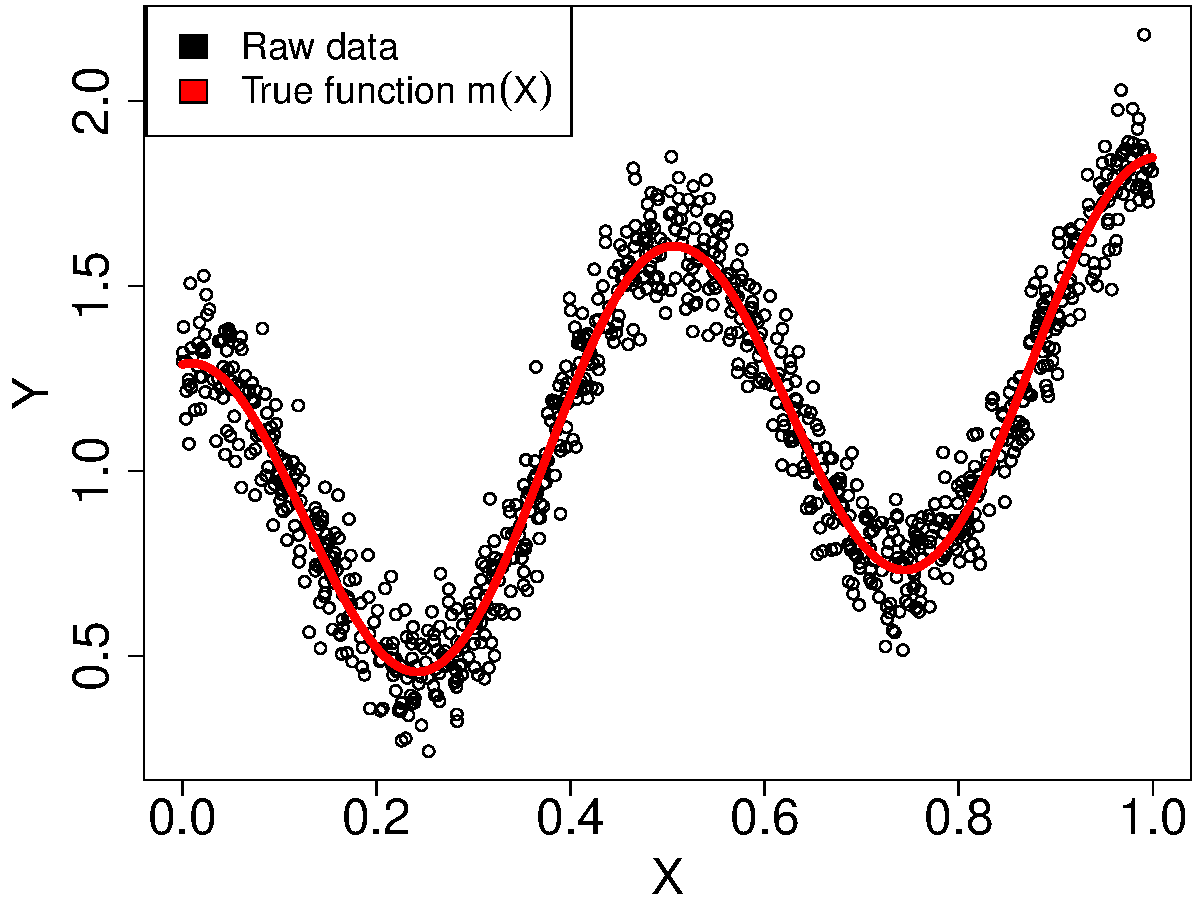
\includegraphics[width=1\linewidth]{Code/Figures/sim1_raw.pdf}
	\end{subfigure}
	\hfil
	\begin{subfigure}[t]{0.49\linewidth}
		\centering
		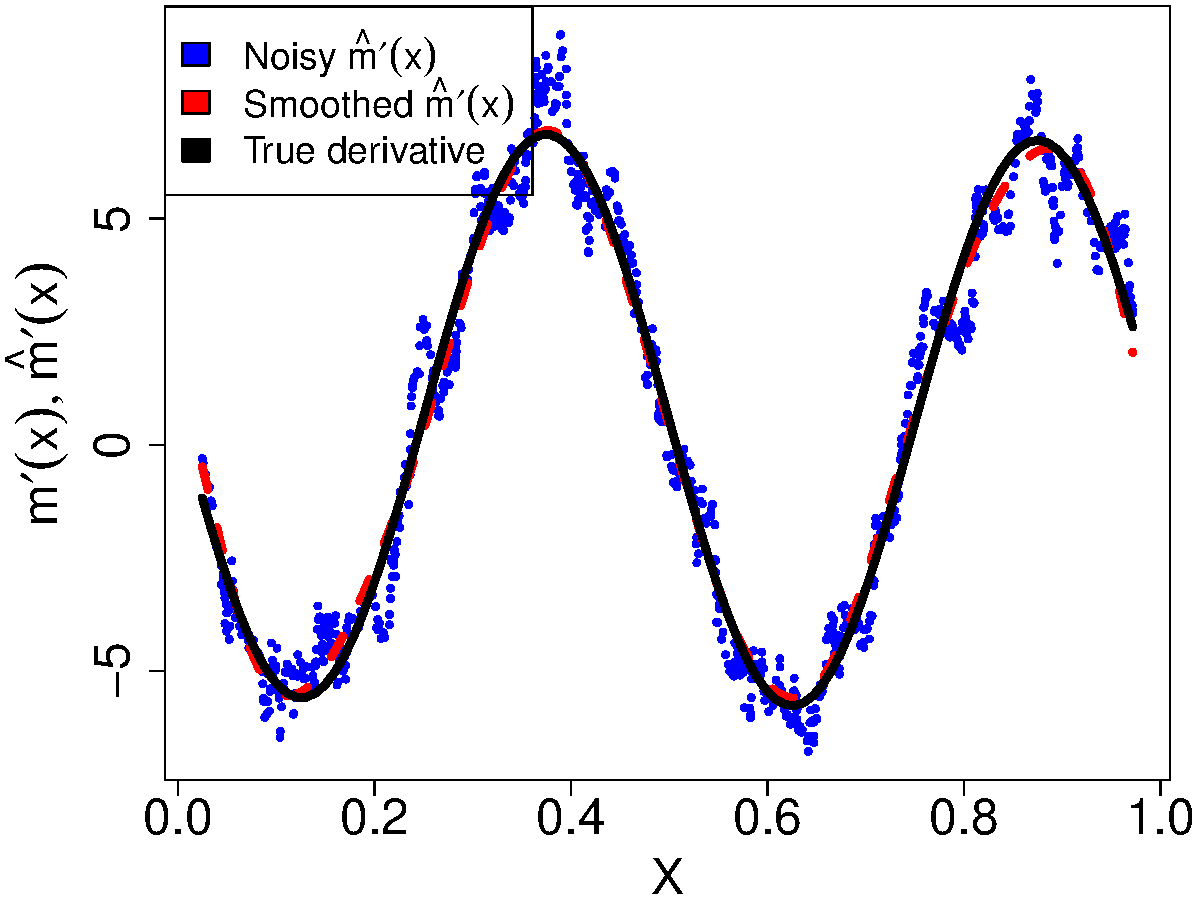
\includegraphics[width=1\linewidth]{Code/Figures/sim1_deriv_x.pdf}
	\end{subfigure}
	\caption{Simulated data $\{(X_i,Y_i)\}_{i=1}^{1000}$ from model \eqref{rand_design} with the first-order noisy derivatives and proposed smoothed derivative estimates. The left panel plots the raw data with $m(X) = \cos^2(2\pi X) + \log(4/3 +X), X\sim \mathrm{Unif}(0,1)$ and $e\sim N(0,0.1^2)$. The right panel shows the first-order noisy derivatives, the proposed smoothed derivative estimator with $k=26$, and the true derivative $m^{(1)}(X)$. (This figure is extended from Figure 1(a) and Figure 2(b) in the paper.)}
	\label{fig:sim1}
\end{figure}

% Major challenge
The main challenge of the derivative estimation problem is a lack of specific data for the derivatives of $m(x)$, in that only the data from model \eqref{rand_design} are given. Such an unavailability of derivative data also makes the parameter tuning and model selection more difficult in the context of derivative estimation. One straightforward proposal for estimating the derivatives is to derive an estimator $\hat{m}(x)$ of the regression function and take its derivatives. Nevertheless, the performance of such a derivative estimator relies heavily on how well the original regression function is estimated, and the estimation errors accumulate as the orders of derivatives increase \citep{de2013derivative}. 

\begin{figure}
	\centering
	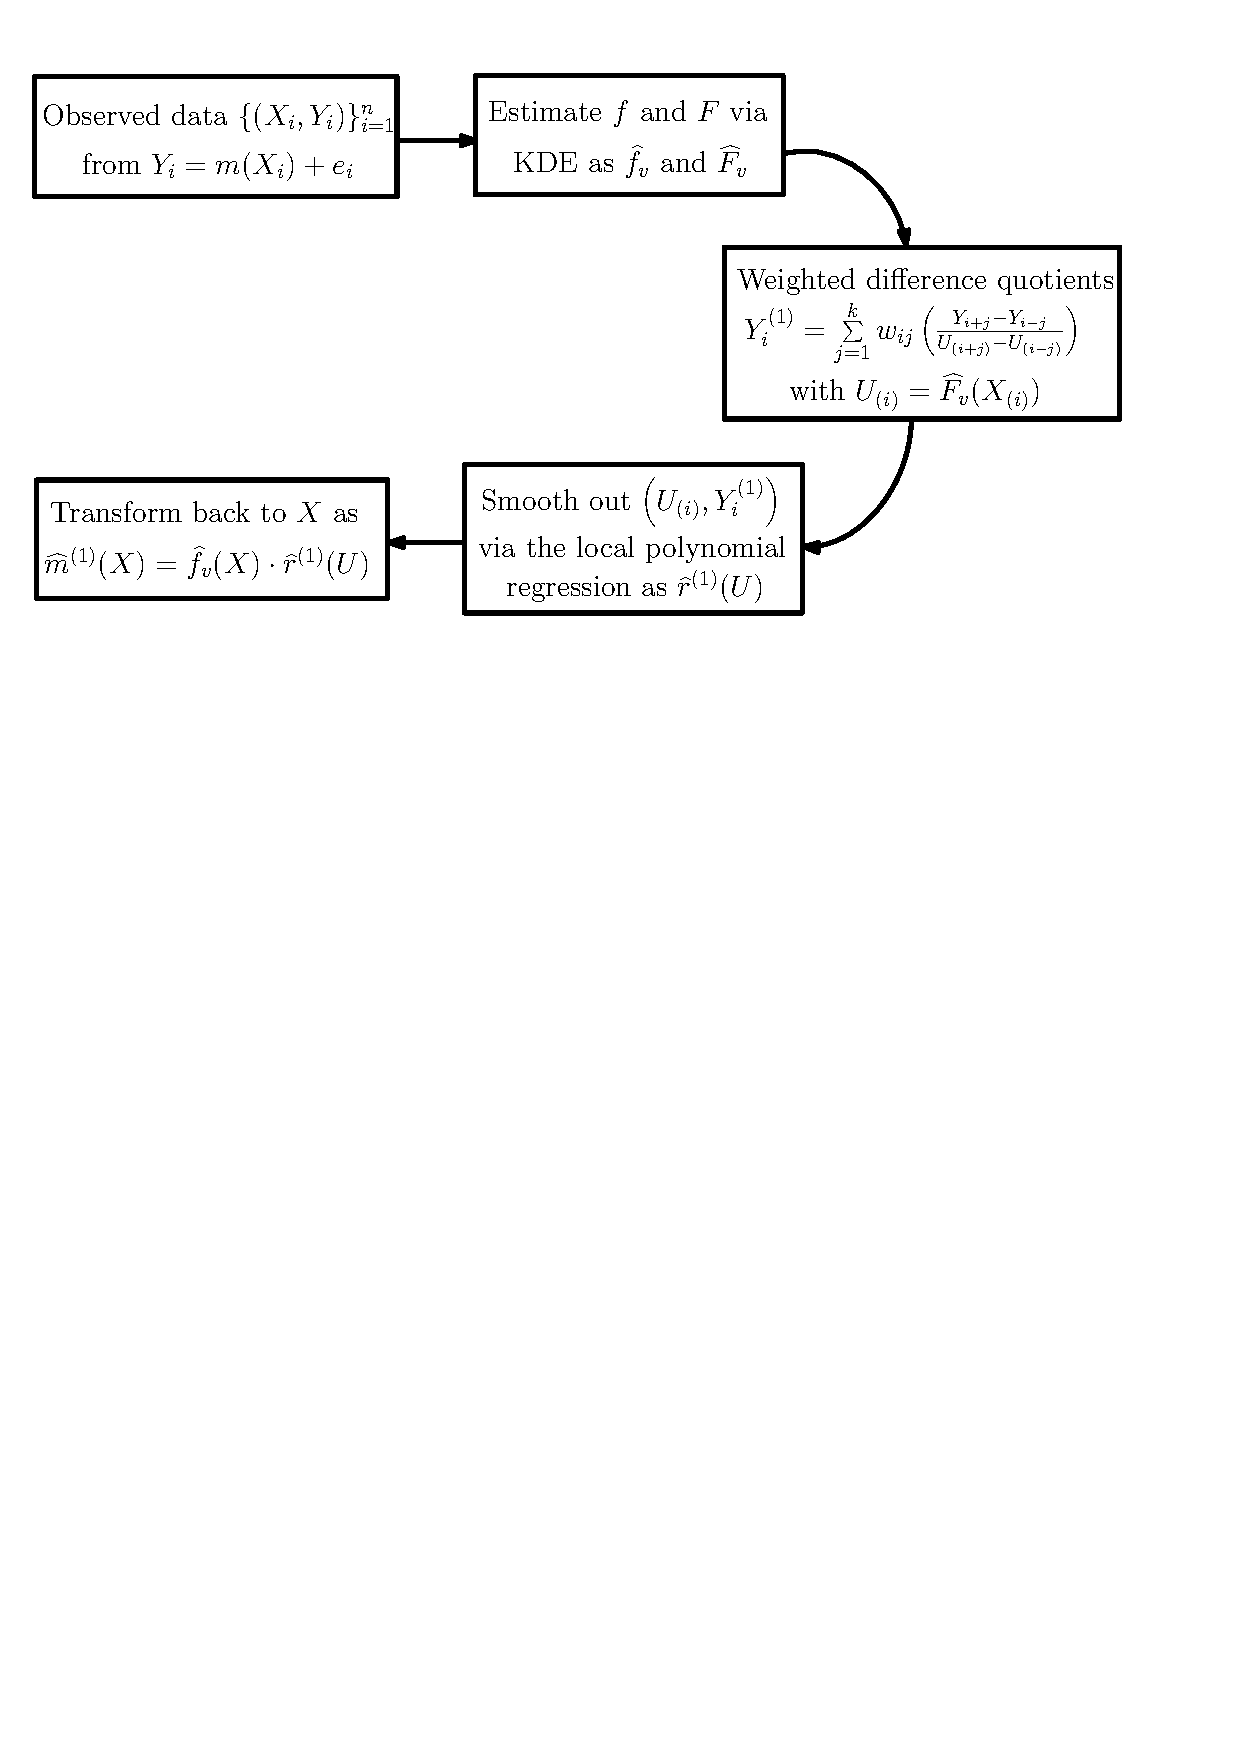
\includegraphics[width=0.85\linewidth]{Code/Figures/method_flow.pdf}
	\caption{Summary of the derivative estimation framework in the paper.}
	\label{fig:method_summary}
\end{figure}

Our discussed paper \citep{liu2020smoothed}, which is an extended version of \cite{liu2018derivative}, tackles the above challenges by proposing a data-driven method for estimating derivatives directly from the observed data $\{(X_i,Y_i)\}_{i=1}^n$; see Section~\ref{Sec:method}. It extends the framework proposed by \cite{de2013derivative} from the equispaced design, where $X_i=a+\frac{(i-1)(b-a)}{n-1},i=1,...,n$, to the random design as model \eqref{rand_design}. In particular, a set of empirical derivatives is constructed through weighted difference quotients, and the local polynomial regression for correlated errors \citep{de2018local} is utilized to smooth out these noisy derivatives; see \autoref{fig:method_summary} for a brief methodological summary and the right panel of \autoref{fig:sim1} for an example. One crucial difference between the equispaced and random designs is that a basic assumption called the symmetric property $x_{i+j}-x_i=x_i-x_{i-j}$ no longer holds for the random design \eqref{rand_design}. Overcoming this difficulty and deriving asymptotic properties become the main contributions of the paper; see Section~\ref{Sec:asymp_res}. Given that the paper only presents the asymptotic properties under the uniformly distributed covariate on $[0,1]$, we derive the pointwise and uniform rates of convergence for the proposed derivative estimators when the unknown distribution of $X$ is estimated by the kernel density estimator (KDE; \citealt{rosenblatt1956remarks,parzen1962estimation,chen2017tutorial}) as an extension; see Section~\ref{Sec:extension}. While the authors of the paper did not make any code publicly available, we reproduce all of their simulation studies and supplement a real-world application in Section~\ref{Sec:experiments} and Appendix~\ref{App:repro}. The reproducible code and a new \texttt{Python} implementation are available at \url{https://github.com/zhangyk8/NonDeriDQ}.
%\begin{enumerate}
%	\item The asymptotic rates of convergence of the empirical first-order derivatives $\hat{Y}_i$ for $k+1\leq i\leq n-k$ are given by
%\end{enumerate}

\subsection{Other Related Literature}
\label{Sec:related_work}

In the regime of derivative estimation, parametric methods are rarely used because it is difficult to propose a valid parametric family that explains the data. The only related literature on parametric derivative estimation appears to be in signal processing \citep{belkic2018validation}, where a complicated form of the fast Pad\'e transform was applied. Even when it is common to estimate the variogram via parametric models in spatial statistics, \cite{gorsich2000variogram} still advocated for nonparametric derivative estimation in order to assist the variogram model selection. We briefly review the major nonparametric derivative estimation methods as follows, where the optimal rate of convergence for a nonparametric derivative estimator was studied by \cite{stone1980optimal,stone1982optimal}. 

$\bullet$ {\bf Regression/Smoothing splines:} The spline regression \citep{deboor1968splines} approximates the regression function $m(x)$ by a linear basis expansion as $f(x) = \sum_{j=1}^M \beta_j g_j(x)$, where $\{g_j:\mathbb{R}\to \mathbb{R}\}_{j=1}^M$ are polynomial transformations of $x$ and $\bm{\beta} = (\beta_1,...,\beta_M)^T \in \mathbb{R}^M$ is obtained from the least-square solution under some knot constraints or using B-splines; see Chapter 5 of \cite{hastie2009elements}. The $L_2$ rate of convergence for derivative estimators based on regression splines was derived in \cite{stone1985additive}. Other asymptotic properties, including bias, variance, and normality, of the derivatives of regression splines for estimating the derivatives of $m(x)$ were studied by \cite{zhou2000derivative}. As for smoothing splines, one will search for the solution that minimizes the penalized residual sum of squares $\sum_{i=1}^n \left[Y_i-f(X_i)\right]^2 + \lambda \int \left[f''(t)\right]^2 dt$ among all functions $f(x)$ with twice continuous derivatives, which can be shown to be a natural cubic spline with knots at $\{X_i\}_{i=1}^n$ and $\hat{f}(x)=\sum_{i=1}^n \hat{\beta}_j g_j(x)$ can be obtained by the usual penalized least-square solution \citep{hastie2009elements}. Estimating the derivatives $m^{(q)}(x), q=1,2,...$ via the derivatives of smoothing splines may not be ideal, since the smoothing parameter depends on the order of the derivative \citep{wahba1990optimal}. In the case of semiparametric penalized splines, \cite{jarrow2004estimating} indeed noticed that more smoothing is required for derivative estimation than the smoothing parameter selected by generalized cross-validation.

$\bullet$ {\bf Gasser-M{\"u}ller derivative estimator:} There were also some research works about kernel-based derivative estimation methods. Given the i.i.d. sample $\{(X_i,Y_i)\}_{i=1}^n$ from model \eqref{rand_design}, one particular example method is based on the Gasser-M{\"u}ller regression estimator \citep{gasser1979kernel} as $\hat{m}_{h,GM}(x) = \frac{1}{h} \sum_{i=1}^n Y_i\cdot \int_{s_{i-1}}^{s_i} K\left(\frac{x-u}{h}\right) du$, where $s_i=\frac{X_{(i)}+X_{(i+1)}}{2}$ for $i=1,...,n$ with $X_{(0)}=-\infty$ and $X_{(n+1)}=\infty$, $K:\mathbb{R}\to [0,\infty)$ is the kernel function, and $h>0$ is the bandwidth parameter. \cite{gasser1984estimating} considered using the $q$-th order derivative of $\hat{m}_h(x)$ as $\hat{m}_{h,GM}^{(q)}(x) = \frac{1}{h^{q+1}} \sum\limits_{i=1}^n Y_i\int_{s_{i-1}}^{s_i} K^{(q)}\left(\frac{x-u}{h}\right) du$ to estimate the true derivative $m^{(q)}(x)$ of the regression. A robust variant of the Gasser-M{\"u}ller derivative estimator was also discussed in \cite{hardle1985robust}.

$\bullet$ {\bf Nadaraya-Watson derivative estimator:} Another well-known kernel-based derivative estimator stems from Nadaraya-Watson regression estimator \citep{nadaraya1964estimating,watson1964smooth}. Instead of using the derivative of Nadaraya-Watson regression estimator, \cite{mack1989derivative} proposed a simpler variant as $\hat{m}_{h,NW}^{(q)}(x) = \frac{1}{nh^{q+1}} \sum\limits_{i=1}^n \frac{Y_i \cdot K^{(q)}\left(\frac{x-X_i}{h}\right)}{\hat{f}_v(X_i)}$, where $\hat{f}_v$ is the KDE for the density $f$ of $X$ in model \eqref{rand_design} with the bandwidth parameter $v>0$.

Some uniform consistency properties of these kernel-based derivative estimators were also analyzed by \cite{delecroix1996nonparametric}. For their bandwidth selection, \citet{rice1986bandwidth,muller1987bandwidth} proposed a generalized cross-validation criterion that utilizes the difference quotients introduced below and a factor method that relies on a careful choice of kernel functions.

$\bullet$ {\bf Local polynomial regression:} Local polynomial regression \citep{fan1996local} generalizes Nadaraya-Watson estimator and leads to an intuitive estimate for the $q$-th order derivative $m^{(q)}(x)$. The idea is from Taylor's theorem \citep{rudin1976principles}, where under smoothness conditions, the regression function $m(x_0)$ can be locally approximated by a polynomial of order $p>q$ as $
m(x_0)\approx \sum_{j=0}^p \frac{m^{(j)}(x)}{j!}(x_0-x)^j \equiv \sum_{j=0}^p \beta_j(x)\left(x_0-x\right)^j.$ 
The coefficients $\hat{\bm{\beta}}(x)=\left(\hat{\beta}_0(x),...,\hat{\beta}_p(x)\right)^T\in \mathbb{R}^{p+1}$ of the fitted polynomial at point $x\in \mathbb{R}$ can be obtained by solving the following weighted least-square problem as:
\begin{equation}
\label{loc_pol}
\begin{split}
\hat{\bm{\beta}}(x) &=\argmin_{\bm{\beta}(x)\in \mathbb{R}^{p+1}} \sum_{i=1}^n \left[Y_i - \sum_{j=0}^p \beta_j(x)\cdot (X_i -x)^j \right]^2 K\left(\frac{X_i-x}{h}\right) \\
&= \argmin_{\bm{\beta}(x)\in \mathbb{R}^{p+1}} \left\{\left[\bm{Y} - \bm{X}\bm{\beta}(x)\right]^T \bm{W} \left[\bm{Y} - \bm{X}\bm{\beta}(x)\right] \right\},
\end{split}
\end{equation}
where $K:\mathbb{R}\to [0,\infty)$ is the kernel function, $h>0$ is the smoothing bandwidth parameter, and  
$$\bm{Y} = \begin{pmatrix}
Y_1\\
\vdots\\
Y_n
\end{pmatrix}, \quad \bm{X} = \begin{pmatrix}
1 & (X_1-x) & \cdots & (X_1-x)^p\\
\vdots & \vdots & \ddots & \vdots\\
1 & (X_n-x) & \cdots & (X_n-x)^p\\
\end{pmatrix}, \quad \bm{W} = \begin{pmatrix}
K\left(\frac{X_1-x}{h}\right) & & \\
& \ddots & \\
& & K\left(\frac{X_n-x}{h}\right)
\end{pmatrix}.$$
Thus, $\hat{\bm{\beta}}(x) = \left(\bm{X}^T\bm{W}\bm{X}\right)^{-1} \bm{X}^T \bm{W}\bm{Y}$. Moreover, $\hat{m}^{(q)}(x) = q!\cdot\hat{\beta}_q(x)$ is a natural estimator for the derivatives $m^{(q)}(x), q=0,1,...,p$. 


$\bullet$ {\bf Difference quotient based methods:} It is natural from the definition \eqref{deriv_def} to apply the (first-order) difference quotients $\hat{q}_i^{(1)} = \frac{Y_i - Y_{i-1}}{X_{(i)}- X_{(i-1)}}, i=2,...,n$ (also called Newton's quotients; \citealt{lang1968analysis}) to estimating the first-order derivative \citep{muller1987bandwidth,hardle1990applied,charnigo2011generalized}, where $X_{(1)}\leq \cdots \leq X_{(n)}$ are order statistics of $\{X_i\}_{i=1}^n$ and $Y_i,i=1,...,n$ are also reordered according to $\{X_{(i)}\}_{i=1}^n$. However, the variances of difference quotients are (stochastically) proportional to $n^2$ under some smoothness conditions on $m$ and noises with nonzero variances as in model \eqref{rand_design}; see Section 2.1 in \cite{de2013derivative} and our Remark~\ref{remark:O_n} in Appendix~\ref{App:auxi_res}. In order to reduce the variance, \cite{iserles2009first} considered aggregating several symmetric difference quotients by linear combinations as:
\begin{equation}
\label{weight_DQ}
\hat{Y}_i^{(1)} = \sum_{j=1}^k w_{i,j}\left(\frac{Y_{i+j} - Y_{i-j}}{X_{(i+j)} - X_{(i-j)}}\right) \quad \text{ with } \quad \sum_{j=1}^k w_{i,j}=1 \quad \text{ for } i=k+1,...,n-k,
\end{equation}
where $k \leq \frac{n-1}{2}$ is a tuning parameter and the weights $w_{i,j}, j=1,...,k$ for each $i$ are chosen by minimizing the variance $\mathrm{Var}(\hat{Y}_i^{(1)})$. The idea of weighted difference quotients has been employed in derivative estimation by \cite{de2013derivative,wang2015derivative}, and \cite{dai2016optimal} further generalizes this idea by formulating a constrained optimization problem for obtaining the weights. All these works focus on the equispaced design, and it is unclear how to extend their methods to the random design. 


\section{Derivative Estimation via Weighted Difference Quotients}
\label{Sec:method}

In this section, we present the methodology of estimating first and second order derivatives via weighted difference quotients \eqref{weight_DQ} and local polynomial smoothing in the discussed paper. 

\subsection{Probability Integral Transform to the Uniform Distribution}
\label{Sec:PIT}

Recall model \eqref{rand_design} that generates our i.i.d. data $\{(X_i,Y_i)\}_{i=1}^n$, where the covariate $X$ has density $f$ and CDF $F$. It is well-known \citep{casella2002statistical} that $F(X_i), i=1,...,n$ follows the uniform distribution $\mathrm{Unif}[0,1]$. Thus, it suffices to estimate the derivatives of a transformed regression function $r(U) = m(F^{-1}(U))$ and refer back to the derivatives of the original regression function $m(X) = r(F(X))$ through the chain rules as:
\begin{equation}
\label{back_transform}
\begin{split}
m^{(1)}(X)=\frac{d m(X)}{dX} &= \frac{d r(U)}{dU} \cdot \frac{dU}{d X} = f(X) \cdot r^{(1)}(U),\\
m^{(2)}(X)=\frac{d^2 m(X)}{dX^2} &= \frac{d}{dX}\left(f(X) \cdot \frac{dr(U)}{dU} \right) = f^{(1)}(X) \cdot r^{(1)}(U) + \left[f(X)\right]^2 r^{(2)}(U).
\end{split}
\end{equation}
While $F(X),f(X),f^{(1)}(X)$ are unknown in practice, they can be estimated by the KDE as:
\begin{equation}
\label{KDE}
\hat{f}_v(X)=\frac{1}{nv} \sum_{i=1}^n K_{\text{kde}}\left(\frac{X-X_i}{v}\right), \quad \hat{F}_v(X) = \frac{1}{nv} \sum_{i=1}^n \int_{-\infty}^X K_{\text{kde}}\left(\frac{u-X_i}{v}\right) du,
\end{equation} 
and $\hat{f}_v^{(1)}(X) = \frac{1}{nv^2} \sum\limits_{i=1}^n K_{\text{kde}}^{(1)}\left(\frac{X-X_i}{v}\right)$, where $K_{\text{kde}}:\mathbb{R}\to [0,\infty)$ is the kernel function and $v>0$ is the bandwidth parameter. In the paper, the Gaussian kernel $K_{\text{kde}}(u)=\frac{1}{\sqrt{2\pi}} \exp\left(-\frac{u^2}{2}\right)$ is applied, and the bandwidth $v$ is selected by the two-stage plug-in method \citep{sheather1991reliable}; see also Section 3.6 in \cite{wand1994kernel}. Practically, these quantities can be obtained from the \texttt{R} functions \texttt{kde}, \texttt{kcde}, \texttt{kdde} with default parameters in the \texttt{R} package \texttt{ks} \citep{ks2022R}.

\subsection{First-Order Noisy Derivative Estimator}

Given that the observed covariates $\{X_i\}_{i=1}^n$ can be transformed into (approximately) uniformly distributed random variables on $[0,1]$ as shown in Section~\ref{Sec:PIT}, we consider the i.i.d. data $\{(U_i,Y_i)\}_{i=1}^n$ with $U_i\sim \mathrm{Unif}[0,1], i=1,...,n$ in the sequel. Furthermore, we order the data $\{(U_i,Y_i)\}_{i=1}^n$ according to the magnitude of $U_i,i=1,...,n$ so that the model \eqref{rand_design} becomes
\begin{equation}
\label{rand_design_unif}
Y_i=r(U_{(i)}) + e_i, \quad i=1,...,n,
\end{equation}
where $r(u)=\mathbb{E}\left[Y|U=u\right] = m(F^{-1}(u))$ has the same role as the regression function $m(x)$ in \eqref{rand_design} and $U_{(1)} \leq U_{(2)} \leq \cdots \leq U_{(n)}$ are order statistics. Based on \eqref{weight_DQ}, the proposed first-order derivative estimator for the random design at $u=U_{(i)}$ is defined as:
\begin{equation}
\label{weight_diff_quo}
\hat{Y}_i^{(1)} = \sum_{j=1}^k w_{i,j} \left(\frac{Y_{i+j} - Y_{i-j}}{U_{(i+j)} - U_{(i-j)}}\right) \quad \text{ for } \quad k+1\leq i \leq n-k, 
\end{equation}
where $k \leq \frac{n-1}{2}$ is the tuning parameter and the weights are given by
$w_{i,j} = \frac{\left(U_{(i+j)} - U_{(i-j)}\right)^2}{\sum_{\ell=1}^k \left(U_{(i+\ell)} - U_{(i-\ell)}\right)^2}$ for $j=1,...,k$ that minimize the variance of \eqref{weight_diff_quo}; see Proposition~\ref{prop:weight_first} in Appendix~\ref{App:auxi_res}. Notice that the $j$-th weight $w_{i,j}$ is proportional to the reciprocal variance of the difference quotient $\frac{Y_{i+j} - Y_{i-j}}{U_{(i+j)} - U_{(i-j)}}$ and incorporates the equispaced design on $[a,b]$ satisfying $U_{(i+j)} - U_{(i-j)} = \frac{2j(b-a)}{(n-1)}$ for $j=1,...,k$ in \cite{charnigo2011generalized,de2013derivative} as a special case. 

$\bullet$ {\bf Boundary Correction:} The proposed estimator \eqref{weight_diff_quo} is only valid at $U_{(i)}$ for $k+1\leq i \leq n-k$. Within the left and right boundary regions $2\leq i \leq k$ and $n-k+1\leq i \leq n-1$, one may consider using $k(i)$ weighted difference quotients in \eqref{weight_diff_quo} instead, where $k(i)=i-1$ for the left boundary and $k(i)=n-i$ for the right boundary. However, the asymptotic variance of $\hat{Y}_i^{(1)}$ is $O_P\left(\frac{3\sigma_e^2 (n+1)^2}{k(i)(k(i)+1)(2k(i)+1)}\right)$ and will become $O_P(n^2)$ when $i$ is close to 2 and $n-1$; see \autoref{thm:asym_first} in Section~\ref{Sec:first_asymp}. To reduce the variance of $\hat{Y}_i^{(1)}$ within the boundary regions, the paper proposes a boundary corrected estimator as:
\begin{equation}
\label{weight_diff_quo_bnd}
\hat{Y}_i^{(1)} = \sum_{j=1}^{k(i)} w_{i,j} \left(\frac{Y_{i+j} - Y_{i-j}}{U_{(i+j)} - U_{(i-j)}}\right) + \sum_{j=k(i)+1}^k w_{i,j} \left[\left(\frac{Y_{i+j} - Y_i}{U_{(i+j)} - U_{(i)}}\right) \mathbbm{1}_{\{2\leq i\leq k\}} + \left(\frac{Y_i - Y_{i-j}}{U_{(i)} - U_{(i-j)}}\right) \mathbbm{1}_{\{n-k< i< n\}} \right],
\end{equation}
where 
\[
w_{i,j} = \begin{cases}
\frac{\left(U_{(i+j)} - U_{(i-j)}\right)^2}{\sum_{\ell=1}^{k(i)} \left(U_{(i+\ell)} - U_{(i-\ell)}\right)^2 + \sum_{\ell=k(i)+1}^k \left[\left(U_{(i+\ell)} - U_{(i)}\right)^2 \mathbbm{1}_{\{2\leq i\leq k\}} + \left(U_{(i)} - U_{(i-\ell)}\right)^2 \mathbbm{1}_{\{n-k< i< n\}} \right]}, & 1\leq j\leq k(i),\\
\frac{\left(U_{(i+j)} - U_{(i)}\right)^2 \mathbbm{1}_{\{2\leq i\leq k\}} + \left(U_{(i)} - U_{(i-j)}\right)^2 \mathbbm{1}_{\{n-k < i < n\}}}{\sum_{\ell=1}^{k(i)} \left(U_{(i+\ell)} - U_{(i-\ell)}\right)^2 + \sum_{\ell=k(i)+1}^k \left[\left(U_{(i+\ell)} - U_{(i)}\right)^2 \mathbbm{1}_{\{2\leq i\leq k\}} + \left(U_{(i)} - U_{(i-\ell)}\right)^2 \mathbbm{1}_{\{n-k< i< n\}} \right]}, & k(i)< j\leq k.
\end{cases}
\]
We also take $\hat{Y}_1^{(1)} = \hat{Y}_2^{(1)}$ and $\hat{Y}_n^{(1)} = \hat{Y}_{n-1}^{(1)}$. In the worst-case scenario, the variance of $\hat{Y}_i^{(1)}$ given by \eqref{weight_diff_quo_bnd} reduces to $O_P\left(\frac{n^2}{k^2}\right)$ and its bias is still of the order $O_P\left(\frac{k}{n}\right)$. 


\subsection{Second-Order Noisy Derivative Estimator}

Under model \eqref{rand_design_unif}, the proposed second-order derivative estimator is defined as:
\begin{equation}
\label{weighted_DQ_second}
\hat{Y}_i^{(2)} = 2\sum_{j=1}^{k_2} w_{ij,2} \cdot \frac{\left(\frac{Y_{i+j+k_1} -Y_{i+j}}{U_{(i+j+k_1)} - U_{(i+j)}} - \frac{Y_{i-j-k_1} -Y_{i-j}}{U_{(i-j-k_1)} - U_{(i-j)}} \right)}{U_{(i+j+k_1)} + U_{(i+j)} - U_{(i-j-k_1)} -U_{(i-j)}} \quad \text{ for } \quad k_1+k_2 +1 \leq i\leq n-k_1-k_2,
\end{equation}
where $k_1,k_2$ are tuning parameters and $\sum_{j=1}^{k_2} w_{ij,2}=1$. As in the first-order derivative estimator \eqref{weight_diff_quo}, the exact $j$-th weight $\tilde{w}_{ij,2}$ will be proportional to the reciprocal variance of the $j$-th weighted difference terms conditional on $\{U_{(i)}\}_{i=1}^n$ as:
$$\tilde{w}_{ij,2} \propto \frac{1}{\mathrm{Var}\left[\frac{\left(\frac{Y_{i+j+k_1} -Y_{i+j}}{U_{(i+j+k_1)} - U_{(i+j)}} - \frac{Y_{i-j-k_1} -Y_{i-j}}{U_{(i-j-k_1)} - U_{(i-j)}} \right)}{U_{(i+j+k_1)} + U_{(i+j)} - U_{(i-j-k_1)} -U_{(i-j)}} \bigg| U_{(i)},i=1,...,n \right]} \quad \text{ for } \quad j=1,...,k_2.$$
To simplify the estimation procedure, the paper considers taking the asymptotic dominating order of $\tilde{w}_{ij,2}$ as the actual weight $w_{ij,2}=\frac{(2j+k_1)^2}{\sum_{j=1}^{k_2} (2j+k_1)^2}$ in \eqref{weighted_DQ_second}, in the sense that $\tilde{w}_{ij,2} = w_{ij,2}\left\{1+o_P(1)\right\}$ as $k_1,k_2 \to \infty$ by Lemma~\ref{lem:unif_asym} in Appendix~\ref{App:auxi_res}. In addition, given that the boundary correction estimator \eqref{weight_diff_quo_bnd} is too complicated to implement for the second-order derivative estimator \eqref{weighted_DQ_second}, the paper only utilizes the maximum numbers $k_1(i),k_2(i)$ of the available first and second order difference quotients to construct $\hat{Y}_i^{(2)}$ within the boundary regions $i\leq k_1+k_2$ and $i> n-k_1-k_2$. 

\subsection{Smoothing the Noisy Derivatives Through Local Polynomial Regression}
\label{Sec:loc_poly}

The above empirical/noisy derivative estimators \eqref{weight_diff_quo}, \eqref{weight_diff_quo_bnd}, and \eqref{weighted_DQ_second} are only defined at the design points $\{U_{(i)}\}_{i=1}^n$ and would contain noises from the error terms $e_i,i=1,...,n$ in \eqref{rand_design_unif}. To extrapolate beyond the design points and reduce noises, the paper considers applying the local polynomial regression to the interior noisy derivative data $\{(U_{(i)}, \hat{Y}_i^{(1)})\}_{i=k+1}^{n-k}$ for the first order and $\{(U_{(i)}, \hat{Y}_i^{(2)})\}_{i=k_1+k_2+1}^{n-k_1-k_2}$ for the second order. Specifically, in the case of smoothing the first-order derivative estimator \eqref{weight_diff_quo}, we recall from Section~\ref{Sec:related_work} that the local polynomial estimator at point $u_0\in [0,1]$ for estimating the derivative $r^{(1)}(u_0)$ in model \eqref{rand_design_unif} is given by
\begin{equation}
\label{loc_poly_first}
\hat{r}^{(1)}(u_0) = \bm{\epsilon}_1^T \hat{\bm{\beta}}(u_0) = \bm{\epsilon}_1^T \bm{S}_{u_0}^{-1} \bm{U}_{u_0}^T \bm{W}_{u_0} \hat{\bm{Y}}^{(1)},
\end{equation}
where $\bm{\epsilon}_1=(1,0,...,0)^T \in \mathbb{R}^{p+1}$, $\hat{\bm{Y}}^{(1)} = \left(\hat{Y}_{k+1}^{(1)},...,\hat{Y}_{n-k}^{(1)}\right)^T \in \mathbb{R}^{n-2k}$, $\bm{S}_{u_0}=\bm{U}_{u_0}^T \bm{W}_{u_0} \bm{U}_{u_0} \equiv \bm{S}_{n-2k}$, and 
$$\bm{U}_{u_0} = \begin{pmatrix}
	1 & \left(U_{(k+1)}-u_0\right) & \cdots & \left(U_{(k+1)}-u_0\right)^p\\
	\vdots & \vdots & \ddots & \vdots\\
	1 & \left(U_{(n-k)}-u_0\right) & \cdots & \left(U_{(n-k)}-u_0\right)^p\\
\end{pmatrix}, \quad \bm{W}_{u_0} = \begin{pmatrix}
	K\left(\frac{U_{(k+1)}-u_0}{h}\right) & & \\
	& \ddots & \\
	& & K\left(\frac{U_{(n-k)}-u_0}{h}\right)
\end{pmatrix}.$$
To smooth out the second-order derivative estimator \eqref{weighted_DQ_second}, we similarly define the local polynomial estimator
\begin{equation}
\label{local_poly_second}
\hat{r}^{(2)}(u_0) = \bm{\epsilon}_1^T \bm{S}_{u_0}^{-1} \bm{U}_{u_0}^T \bm{W}_{u_0} \hat{\bm{Y}}^{(2)},
\end{equation}
where $\hat{\bm{Y}}^{(2)} = \left(\hat{Y}_{k_1+k_2+1}^{(2)},...,\hat{Y}_{n-k_1-k_2}^{(2)}\right)$, while $\bm{U}_{u_0},\bm{W}_{u_0}$ and $\bm{S}_{u_0}=\bm{U}_{u_0}^T \bm{W}_{u_0} \bm{U}_{u_0} \equiv \bm{S}_{n-2k_1-2k_2}$ are defined through the data $\{(U_{(i)}, \hat{Y}_i^{(2)})\}_{i=k_1+k_2+1}^{n-k_1-k_2}$.

One caveat in applying the local polynomial regression \eqref{loc_poly_first} is that $\left\{\hat{Y}_i^{(1)}\right\}_{i=k+1}^{n-k}$ are no longer independent even when we condition on $\{U_{(i)}\}_{i=1}^n$. To inspect this fact, one can rewrite the first-order noisy derivative estimator \eqref{weight_diff_quo} as:
$$\hat{Y}_i^{(1)} = \sum_{j=1}^k w_{i,j} \left(\frac{r(U_{(i+j)}) - r(U_{(i-j)})}{U_{(i+j)} - U_{(i-j)}}\right) + \sum_{j=1}^k w_{i,j} \left(\frac{e_{i+j} - e_{i-j}}{U_{(i+j)} - U_{(i-j)}}\right),$$
where we denote the second term by $\sum_{j=1}^k w_{i,j} \left(\frac{e_{i+j} - e_{i-j}}{U_{(i+j)} - U_{(i-j)}}\right)$ as the new error terms for $k+1\leq i \leq n-k$. The first term in the above equation is an approximation of $r^{(1)}(U_{(i)})$ with its absolute bias bounded by $O\left(\frac{k}{n}\right) \to 0$ as $n\to \infty$; see \autoref{thm:asym_first} below. Hence, $\{(U_{(i)}, \hat{Y}_i^{(1)})\}_{i=k+1}^{n-k}$ can be regarded as an (ordered) random sample from the model with correlated errors $\tilde{e}_i,i=k+1,...,n-k$ as:
\begin{equation}
\label{rand_design_first_cor}
\hat{Y}_i^{(1)} = r^{(1)}(U_{(i)}) + \tilde{e}_i,
\end{equation}
where $\mathbb{E}\left[\tilde{e}_i|U_i\right]=0$ and $\mathrm{Cov}\left(\tilde{e}_i,\tilde{e}_j | U_{(i)},U_{(j)} \right) = \sigma_{\tilde{e}}^2 \cdot \rho_n(U_{(i)}-U_{(j)})$ with $\sigma_{\tilde{e}}^2 <\infty$ and $\rho_n$ being a stationary correlation function with $\rho_n(0)=1, \rho_n(u) = \rho_n(-u)$ and $|\rho_n(u)|\leq 1$ for all $u\in \mathbb{R}$. Such correlated error structures complicate the bandwidth selection for the local polynomial smoothing \eqref{loc_poly_first} and deteriorate the performance of the final derivative estimator \citep{opsomer2001nonparametric,de2018local}. To resolve this issue, the paper adopts a two-step procedure proposed by \cite{de2018local} to select the final bandwidth $\hat{h}$ in \eqref{loc_poly_first} as follows.
\begin{enumerate}
	\item We fit a local polynomial regression \eqref{loc_poly_first} using a bimodal kernel $\bar{K}:\mathbb{R}\to [0,\infty)$ with $\bar{K}(0)=0$ and compute a pilot bandwidth $\hat{h}_b$ by minimizing the residual sum of squares (RSS) as:
	\begin{equation}
		\label{band_loc_pol}
		\hat{h}_b = \argmin_{h_b>0} \mathrm{RSS}(h_b) = \argmin_{h_b>0} \left\{\frac{1}{n-2k} \sum_{i=k+1}^{n-k} \left(\hat{r}^{(1)}(U_{(i)}) -\hat{Y}_i^{(1)} \right)^2 \right\},
	\end{equation} 
	given the tuning parameter $k$ is chosen a priori as Corollary~\ref{cor:k_sel} in Section~\ref{Sec:first_asymp}. In the paper, the bimodal Gaussian kernel $\bar{K}(u)=\frac{2u^2}{\sqrt{\pi}} \exp(-u^2)$ is applied.
	
	\item To handle the extra mean squared error caused by the non-optimality of kernels with $\bar{K}(0)=0$, we consider the bandwidth correction as:
	$$\hat{h} = \left\{\frac{\int \left(K_p^{\star}(t)\right)^2 dt \left[\int t^{p+1}\bar{K}_p^{\star}(t) dt \right]^2}{\int \left(\bar{K}_p^{\star}(t)\right)^2 dt \left[\int t^{p+1}K_p^{\star}(t) dt \right]^2}\right\}^{\frac{1}{2p+2}} \hat{h}_b = 1.01431 \hat{h}_b,$$
	where $K_p^{\star}(u), \bar{K}_p^{\star}(u)$ are equivalent kernels defined by $\bar{K}(u)$ and $K(u)$ (see Section 3.2.2 in \citealt{fan1996local}), and the last equality follows by using $\bar{K}(u)=\frac{2u^2}{\sqrt{\pi}} \exp(-u^2)$ and $K(u)=\frac{1}{\sqrt{2\pi}} \exp\left(-\frac{u^2}{2}\right)$ under the local cubic regression with $p=3$.  
\end{enumerate}
The final smoothed derivative estimator \eqref{loc_poly_first} is computed with the unimodal kernel $K$ and selected bandwidth $\hat{h}$. The above bandwidth selection procedure also applies to the local polynomial smoothing of the second-order noisy derivative estimator \eqref{weighted_DQ_second}.

\begin{Remark}
The paper does not address the derivative estimation of order higher than two, because it is unwieldy to generalize the proposed framework and its asymptotic properties. More importantly, the bias of weighted difference quotient estimators accumulate as the derivative order increases under the random design setting. As a result, the proposed framework is inadequate to estimate the higher-order derivatives of the regression function $m(x)$.
\end{Remark}

\section{Asymptotic Properties of the Proposed Derivative Estimators}
\label{Sec:asymp_res}

In this section, we study the asymptotic conditional bias and variance of the proposed derivative estimators and their smoothed counterparts by local polynomial regression under model \eqref{rand_design_unif}. These asymptotic results suggest some practical guidelines for choosing the tuning parameters $k$ or $k_1,k_2$.

\subsection{First-Order Derivative Estimation}
\label{Sec:first_asymp}

\begin{theorem}[Theorem 1 in \citealt{liu2020smoothed}]
\label{thm:asym_first}
Assume that $r$ is twice continuously differentiable on $[0,1]$ under model \eqref{rand_design_unif}. Then, the conditional bias and variance of the first-order noisy derivative estimator \eqref{weight_diff_quo} given $\mathbb{U} = \left(U_{(i-j)},...,U_{(i+j)}\right)$ for $i>j$ and $i+j\leq n$ are 
\begin{align*}
\left|\mathrm{Bias}\left[\hat{Y}_i^{(1)} \big| \mathbb{U}\right] \right| &\leq \left[\sup_{u\in [0,1]} \left|r^{(2)}(u)\right|\right] \frac{3k(k+1)}{4(n+1)(2k+1)} + o_P\left(\frac{k}{n}\right),\\
\mathrm{Var}\left[\hat{Y}_i^{(1)} \big| \mathbb{U}\right] &= \frac{3\sigma_e^2 (n+1)^2}{k(k+1)(2k+1)} + o_P\left(\frac{n^2}{k^3}\right)
\end{align*}
uniformly for $k+1\leq i\leq n-k$ when $k\to \infty$ as $n\to \infty$. Further, if we assume that $r$ is $q+1$ times continuously differentiable on $[0,1]$ for $q\geq 1$, then the asymptotic order of the exact conditional bias is given by
\[
\mathrm{Bias}\left[\hat{Y}_i^{(1)} \big| \mathbb{U}\right]=
\begin{cases}
O_P\left(\frac{k}{n}\right), & q=1,\\
O_P\left(\max\left\{\frac{k^{\frac{1}{2}}}{n},\, \frac{k^2}{n^2}\right\}\right), & q\geq 2.
\end{cases}
\]
\end{theorem}

\noindent The proof of \autoref{thm:asym_first} can be found in Appendix~\ref{App:proof_thm1}. It reveals the following three corollaries:

\noindent$\bullet$ The conditional bias and variance of $\hat{Y}_i^{(1)}$ will tend to 0 if the tuning parameter $k$ tends to infinity in a rate faster than $O\left(n^{\frac{2}{3}}\right)$ but slower than $O\left(n \right)$.
	
\noindent$\bullet$ $\hat{Y}_i^{(1)}$ is a (pointwise) consistent estimator of $r^{(1)}(U_{(i)})$ as $\frac{k}{n} \to 0$ and $\frac{n^2}{k^3}\to 0$.
	
\noindent$\bullet$ The fastest $L_2$ rate of convergence for $\mathbb{E}\left[\left(\hat{Y}_i^{(1)} - r^{(1)}(U_{(i)})\right)^2 \big| \mathbb{U}\right]$ is $O_P\left(n^{-\frac{2}{5}}\right)$ when $k=O\left(n^{\frac{4}{5}}\right)$, which is also the optimal rate of convergence among twice differentiable functions \citep{stone1982optimal}.

\autoref{thm:asym_first} also provides us with a practical guideline for selecting the tuning parameter $k$ in \eqref{weight_diff_quo}. In principle, we will minimize the asymptotic conditional mean integrated squared error (MISE).

\begin{cor}[Corollary 2 in \citealt{liu2020smoothed}]
\label{cor:k_sel}
Let $\mathcal{B} = \sup_{u\in [0,1]} \left|r^{(2)}(u)\right|$. Under the assumptions of \autoref{thm:asym_first}, the tuning parameter $k$ that minimizes the asymptotic upper bound of the conditional MISE is given by
$$k_{\text{opt}} = \argmin_{k=1,2,...,\floor{\frac{n-1}{2}}} \left[\mathcal{B}^2\frac{9k^2(k+1)^2}{16(n+1)^2(2k+1)^2} + \frac{3\sigma_e^2 (n+1)^2}{k(k+1)(2k+1)} \right].$$
\end{cor}

\noindent The proof of Corollary~\ref{cor:k_sel} is given in Appendix~\ref{App:proof_cor2}. To apply Corollary~\ref{cor:k_sel} in practice, the unknown quantity $\mathcal{B} = \sup_{u\in [0,1]} \left|r^{(2)}(u)\right|$ can be approximated by the second-order local slope of a local polynomial regression of order $p=3$ fitted to the data $\{(U_{(i)}, Y_i)\}_{i=1}^n$, while the noise variance $\sigma_e^2$ can be estimated by Hall's $\sqrt{n}$-consistent estimator with the optimal second-order difference sequence \citep{hall1990asymptotically} as $\hat{\sigma}_e^2 = \frac{1}{n-2} \sum_{i=1}^{n-2} \left(0.809Y_i - 0.5Y_{i+1} - 0.309Y_{i+2}\right)^2$. Then, the optimal value $k_{\text{opt}}$ can be obtained by searching over the integer set within $\left[1, \frac{n-1}{2}\right]$.

Now, we study the asymptotic pointwise conditional bias and variance of the smoothed derivative estimator \eqref{loc_poly_first}. Recall from Section~\ref{Sec:loc_poly} that the first-order noisy derivative data $\left\{\left(U_{(i)},\hat{Y}_i^{(1)}\right)\right\}_{i=k+1}^{n-k}$ obtained from \eqref{weight_diff_quo} can be viewed as observations from the additive noise model \eqref{rand_design_first_cor}, where the errors $\tilde{e}_i, i=k+1,...,n-k$ satisfy $\mathbb{E}\left[\tilde{e}_i|U_i\right]=0$ and $\mathrm{Cov}\left(\tilde{e}_i,\tilde{e}_j | U_{(i)},U_{(j)} \right) = \sigma_{\tilde{e}}^2 \cdot \rho_n(U_{(i)}-U_{(j)})$ with $\sigma_{\tilde{e}}^2 <\infty$ and $\rho_n$ being a stationary correlation function with $\rho_n(0)=1, \rho_n(u) = \rho_n(-u)$ and $|\rho_n(u)|\leq 1$ for all $u\in \mathbb{R}$. We make the following assumptions.
\begin{assump}
\label{assump:kernel}
The kernel function $K:\mathbb{R}\to [0,\infty)$ is bounded, symmetric, and Lipschitz continuous at 0. Furthermore, it satisfies $\lim_{|u|\to \infty} |u|^{\ell} K(u) <\infty$ for $\ell=0,...,p$.
\end{assump}
\begin{assump}
\label{assump:cor_func}
The correlation function $\rho_n$ is an element of a sequence $\{\rho_n\}_{n=1}^{\infty}$ with the following properties for all $n\geq 1$: there exist constants $\rho_{\max}, \rho_c >0$ such that $n\int |\rho_n(x)| dx < \rho_{\max}$ and $\lim_{n\to \infty} n \int \rho_n(x) dx =\rho_c$. In addition, for any sequence $\epsilon_n>0$ with $n\epsilon_n\to \infty$, it holds that $n\int_{|x|\geq \epsilon_n} |\rho_n(x)| dx \to 0$ as $n\to \infty$. 
\end{assump}

Assumption~\ref{assump:kernel} is a standard and mild condition for kernel functions \citep{wasserman2006all}. Assumption~\ref{assump:cor_func} requires the correlation to be short-range dependent \citep{opsomer2001nonparametric} and can be satisfies by $\tilde{e}_i,i=k+1,...,n-k$ in model \eqref{rand_design_first_cor} when $k$ is small. Other correlation functions satisfying Assumption~\ref{assump:cor_func} includes $\rho_n(x) = \exp\left(-\alpha n |x|\right)$ and $\rho_n(x)=\frac{1}{1+\alpha n^2 x^2}$ for $\alpha >0$. The asymptotic pointwise conditional bias and variance of $\hat{r}^{(1)}(u_0)$ in \eqref{loc_poly_first} are given in the following theorem.

\begin{theorem}[Theorem 2 in \citealt{liu2020smoothed}]
\label{thm:loc_poly_first}
Assume that $r(\cdot)$ under model \eqref{rand_design_unif} is $(p+2)$ times continuously differentiable in a neighborhood of $u_0$. Under Assumptions~\ref{assump:kernel} and \ref{assump:cor_func}, the conditional bias and variance of \eqref{loc_poly_first} with $u_0\in [0,1]$ for $p$ odd are
\begin{align*}
	\mathrm{Bias}\left[\hat{r}^{(1)}(u_0) | \tilde{\mathbb{U}}\right] &\leq\left[\bm{\epsilon}_1^T \bm{S}^{-1}c_p\cdot \frac{r^{(p+2)}(u_0)}{(p+1)!} \cdot h^{p+1} + \left|\bm{\epsilon}_1^T \bm{S}^{-1} \right|\tilde{c}_p \cdot \frac{3k(k+1) \mathcal{B}}{4(n+1)(2k+1)}\right] \left[1+o_P(1)\right]\\
	&= \left[\left(\int t^{p+1} K_0^{\star}(t) dt\right) \frac{r^{(p+2)}(u_0)}{(p+1)!} \cdot h^{p+1} + \left|\bm{\epsilon}_1^T \bm{S}^{-1}\right| \tilde{c}_p \cdot\frac{3k(k+1) \mathcal{B}}{4(n+1)(2k+1)}\right] \left[1+o_P(1)\right],\\
	\mathrm{Var}\left[\hat{r}^{(1)}(u_0) | \tilde{\mathbb{U}}\right] &= \frac{3\sigma_e^2 (n+1)^2 (1+\rho_c)}{k(k+1)(2k+1) (n-2k) h} \cdot \bm{\epsilon}_1^T \bm{S}^{-1} \bm{S}^* \bm{S}^{-1} \bm{\epsilon}_1 \left[1+o_P(1)\right]\\
	&= \left(\int K_0^{\star}(t)^2 dt \right) \frac{3\sigma_e^2 (n+1)^2 (1+\rho_c)}{k(k+1)(2k+1) (n-2k) h} \left[1+o_P(1)\right]
\end{align*}
as $h\to 0, nh\to \infty, k\to \infty$ with $n\to \infty$, where $\tilde{\mathbb{U}}=\left(U_{(1)},...,U_{(n)}\right)$, $\mathcal{B}=\sup_{u\in [0,1]}\left|r^{(2)}(u) \right|$, $\bm{S}=\left(\mu_{i+j-2}\right)_{1\leq i,j\leq p+1}$ with $\mu_j=\int u^j K(u) du$, $\bm{S}^*=\left(\nu_{i+j-2}\right)_{1\leq i,j\leq p+1}$ with $\nu_j = \int u^j K(u)^2 du$, $c_p=\left(\mu_{p+1},...,\mu_{2p+1} \right)^T$, $\tilde{c}_p=\left(\tilde{\mu}_0,...,\tilde{\mu}_{p} \right)^T$ with $\tilde{\mu}_j=\int |u|^j K(u) du$, $\bm{\epsilon}_1=(1,0,...,0)^T \in \mathbb{R}^{p+1}$, $\left|\bm{\epsilon}_1^T\bm{S}^{-1}\right|$ means elementwise absolute values of $\bm{\epsilon}_1^T\bm{S}^{-1}$, and the equivalent kernel $K_0^{\star}(t) = \bm{\epsilon}_1^T \bm{S}^{-1} \left(1,t,...,t^p\right)^T K(t)$.
\end{theorem}

\noindent The proof of \autoref{thm:loc_poly_first} is in Appendix~\ref{App:proof_thm3}. It implies that the optimal $L_2$ rate of convergence is $O_P\left(n^{-\frac{4p+4}{5p+6}}\right)$, which is attained when $h=O\left(n^{-\frac{2}{5p+6}}\right)$ and $k=O\left(n^{\frac{3p+4}{5p+6}}\right)$; see Remark~\ref{remark:MISE_loc_poly} in Appendix~\ref{App:proof_thm3}. Unlike Corollary~\ref{cor:k_sel}, it is complicated to leverage the bias-variance trade-off in \autoref{thm:loc_poly_first} to select the optimal bandwidth $h$ and tuning parameter $k$ simultaneously, since there are too many unknown quantities that need estimating. Instead, the bandwidth $h$ is selected through a two-step procedure by minimizing the residual sum of squares under a bimodal kernel $\bar{K}$ with an additional correction; recall the details in Section~\ref{Sec:loc_poly}. The rationale behind this procedure is due to the asymptotic equivalence between minimizing $\mathrm{RSS}(h)=\frac{1}{n-2k} \sum_{i=k+1}^{n-k} \left(\hat{r}^{(1)}(U_{(i)}) -\hat{Y}_i^{(1)} \right)^2$ and the sample squared error $\mathrm{SSE}(h) = \frac{1}{n-2k} \sum_{i=k+1}^{n-k} \left(\hat{r}^{(1)}(U_{(i)}) -r^{(1)}(U_{(i)}) \right)^2$ as follows.

\begin{lemma}[Theorem 2 in \citealt{de2018local}]
\label{lem:RSS_SSE}
Under the assumptions in \autoref{thm:loc_poly_first} with a local polynomial regression estimator $\hat{r}^{(1)}$ given by \eqref{loc_poly_first}, if $n^{\delta} \int |\rho_n(t)| dt < \rho_{\delta}$ for $\delta >1$, $p$ is odd, and $h\in \mathcal{H}_n$ with $\mathcal{H}_n=\left[c_1 n^{-\frac{1}{2p+3}},\, c_2 n^{-\frac{1}{2p+3}}\right]$ for some constants $0<c_1<c_2<\infty$, then
$$\mathrm{RSS}(h) = \mathrm{SSE}(h) + \frac{1}{n-2k} \sum_{i=k+1}^{n-k} \tilde{e}_i^2 - \frac{2\sigma_{\tilde{e}}^2\cdot K(0) \cdot \left(\bm{S}^{-1}\right)_{11}\cdot(1 +\rho_c)}{nh} + o_P\left(n^{-\frac{2p+2}{2p+3}}\right),$$
recalling that the domain of $r^{(1)}$ is $[0,1]$ and $\left(\bm{S}^{-1}\right)_{11}$ is the first element in the first row of $\bm{S}^{-1}$.
\end{lemma}

\noindent According to Lemma~\ref{lem:RSS_SSE}, the term related to the correlation structures of errors in model \eqref{rand_design_first_cor} will be removed if we employ a bimodal kernel $\bar{K}$ with $\bar{K}(0)=0$. Hence, $\frac{\mathrm{RSS}(h)}{\mathrm{SSE}(h)} = 1+o_P(1)$ as $n\to\infty$, and we can select the optimal bandwidth by minimizing $\mathrm{RSS}(h)$ without any prior knowledge about the correlation structures of errors.

\subsection{Second-Order Derivative Estimation}

\begin{theorem}[Theorem 3 in \citealt{liu2020smoothed}]
\label{thm:asym_second}
Assume that $r$ is three times continuously differentiable on $[0,1]$ under model \eqref{rand_design_unif}. Then, under the weight $w_{ij,2}=\frac{(2j+k_1)^2}{\sum_{j=1}^{k_2} (2j+k_1)^2}$, the conditional bias and variance of the second-order noisy derivative estimator \eqref{weighted_DQ_second} given $\tilde{\mathbb{U}}=\left(U_{(1)},..., U_{(n)}\right)$ are bounded by
\begin{align*}
\left|\mathrm{Bias}\left[\hat{Y}_i^{(2)} \big| \tilde{\mathbb{U}}\right] \right| &\leq \frac{\sup_{u\in [0,1]}\left|r^{(3)}(u)\right|}{n+1}  \left(\frac{2\sum_{j=1}^{k_2} j^3 + 3k_1 \sum_{j=1}^{k_2} j^2 + \frac{5}{3} k_1^2 \sum_{j=1}^{k_2}j + \frac{1}{3} k_1^3k_2}{4 \sum_{j=1}^{k_2}j^2 + k_1^2k_2 + 4k_1\sum_{j=1}^{k_2} j} \right)\left[1+o_P(1)\right],\\
\mathrm{Var}\left[\hat{Y}_i^{(2)} \big| \tilde{\mathbb{U}}\right] &\leq \frac{4(n+1)^4 \sigma_e^2}{k_1^2 \sum_{j=1}^{k_2} (2j+k_1)^2} \left[1+o_P(1)\right]
\end{align*}
uniformly for $k_1+k_2+1 \leq i\leq n-k_1-k_2$ when $k_1,k_2\to \infty$ as $n\to\infty$.
\end{theorem}

\noindent The proof of \autoref{thm:asym_second} is given in Appendix~\ref{App:proof_thm5}. This theorem implies the following corollaries:
 
$\bullet$ Assuming that $k_1,k_2$ have the same asymptotic order with respect to $n$. The conditional bias and variance of $\hat{Y}_i^{(2)}$ tend to 0 if $k_1,k_2\to\infty$ in a rate faster than $O\left(n^{\frac{4}{5}} \right)$ but slower than $O(n)$.
	
$\bullet$ $\hat{Y}_i^{(2)}$ is a (pointwise) consistent estimator of $r^{(2)}(U_{(i)})$ if $\frac{k_1}{n} \to 0, \frac{k_2}{n} \to 0, \frac{n^4}{k_1^2k_2^3}\to 0$, $\frac{n^4}{k_1^4k_2} \to 0$ as $n\to\infty$; see Remark~\ref{remark:MSE_second_deri} in Appendix~\ref{App:proof_thm5}.
	
$\bullet$ The fastest possible $L_2$ rate of convergence for $\mathbb{E}\left[\left(\hat{Y}_i^{(2)} - r^{(2)}(U_{(i)})\right)^2 \big| \tilde{\mathbb{U}} \right] \to 0$ is $O_P\left(n^{-\frac{2}{7}}\right)$ when $k_1,k_2 = O\left(n^{\frac{6}{7}}\right)$.

Analogous to the first-order derivative estimation through \eqref{weight_diff_quo}, \autoref{thm:asym_second} also sheds light on the bias-variance rationale of selecting the tuning parameters $k_1,k_2$ for the second-order noisy derivative estimator \eqref{weighted_DQ_second}.

\begin{cor}[Corollary 5 in \citealt{liu2020smoothed}]
\label{cor:k1_k2_sel}
Let $\mathcal{B}_2=\sup_{u\in [0,1]} \left|r^{(3)}(u)\right|$. Under the assumptions of \autoref{thm:asym_second}, the tuning parameters $k_1$ and $k_2$ that minimize the asymptotic upper bound of the conditional MISE are
\begin{align*}
\left(k_1,k_2\right)_{\text{opt}} &= \argmin_{k_1,k_2=1,2,...} \left[\frac{\mathcal{B}_2^2}{(n+1)^2}  \left(\frac{2\sum\limits_{j=1}^{k_2} j^3 + 3k_1 \sum\limits_{j=1}^{k_2} j^2 + \frac{5}{3} k_1^2 \sum\limits_{j=1}^{k_2}j + \frac{1}{3} k_1^3k_2}{4 \sum_{j=1}^{k_2}j^2 + k_1^2k_2 + 4k_1\sum_{j=1}^{k_2} j} \right)^2 + \frac{4(n+1)^4\sigma_e^2}{k_1^2\sum\limits_{j=1}^{k_2} (2j+k_1)^2} \right].
\end{align*}
\end{cor}

\noindent The proof of Corollary~\ref{cor:k1_k2_sel} is given in Appendix~\ref{App:proof_cor6}. The unknown quantity $\mathcal{B}_2$ can be approximated by the local polynomial regression estimator with $p=4$, while $\sigma_e^2$ is again estimated by Hall's $\sqrt{n}$-consistent estimator described after Corollary~\ref{cor:k_sel}. Then, the optimal pair $\left(k_1,k_2\right)_{\text{opt}}$ can be obtained by grid-searching over a Cartesian product set $\left\{1,2,...,\floor{\frac{n-1}{2}}\right\} \otimes \left\{1,2,...,\floor{\frac{n-1}{2}}\right\}$.

Finally, we study the asymptotic pointwise conditional bias and variance of the smoothed second-order derivative estimator \eqref{local_poly_second}. As in \eqref{rand_design_first_cor}, the data $\{(U_{(i)}, \hat{Y}_i^{(2)})\}_{i=k_1+k_2+1}^{n-k_1-k_2}$ can also be viewed as an (ordered) random sample from the model $\hat{Y}_i^{(2)} =r^{(2)}(U_{(i)}) + \acute{e}_i$, in which the error terms $\acute{e}_i, i=k_1+k_2+1,...,n-k_1-k_2$ are correlated with $\mathbb{E}\left(\acute{e}_i|U_{(i)}\right)=0, \mathrm{Cov}\left(\acute{e}_i,\acute{e}_j|U_{(i)},U_{(j)}\right) = \sigma_{\acute{e}}^2\cdot \acute{\rho}_n(U_{(i)} - U_{(j)})$ for $i\neq j$, and $\acute{\rho}_n$ is a stationary correlation function with $\acute{\rho}_n(0)=1$,  $\acute{\rho}_n(u)=\acute{\rho}_n(-u)$, and $\left|\acute{\rho}_n(u)\right|\leq 1$ for all $u\in \mathbb{R}$. Analogous to \autoref{thm:loc_poly_first}, we have the following theorem for the asymptotic upper bound of the conditional bias and variance of $\hat{r}^{(2)}(u_0)$ in \eqref{local_poly_second}.

\begin{theorem}[Theorem 4 in \citealt{liu2020smoothed}]
\label{thm:local_poly_second}
Assume that $r(\cdot)$ under model \eqref{rand_design_unif} is $(p+3)$ times continuously differentiable in a neighborhood of $u_0$. Under Assumptions~\ref{assump:kernel} and \ref{assump:cor_func} on $\acute{\rho}_n$, the conditional bias and variance of \eqref{local_poly_second} with $u_0\in [0,1]$ for $p$ odd are
\begin{align*}
	\mathrm{Bias}\left[\hat{r}^{(2)}(u_0) | \tilde{\mathbb{U}}\right] &\leq \Bigg[\left|\bm{\epsilon}_1^T \bm{S}^{-1} \right|\tilde{c}_p\cdot \left(\frac{\mathcal{B}_2}{n+1}\right) \left(\frac{2\sum_{j=1}^{k_2} j^3 + 3k_1 \sum_{j=1}^{k_2} j^2 + \frac{5}{3} k_1^2 \sum_{j=1}^{k_2}j + \frac{1}{3} k_1^3k_2}{4 \sum_{j=1}^{k_2}j^2 + k_1^2k_2 + 4k_1\sum_{j=1}^{k_2} j} \right)\\
	&\quad + \bm{\epsilon}_1^T \bm{S}^{-1} c_p \cdot \frac{r^{(p+3)}(u_0)}{(p+1)!}\cdot h^{p+1} \Bigg] \left[1+o_P(1)\right]\\
	\mathrm{Var}\left[\hat{r}^{(2)}(u_0) | \tilde{\mathbb{U}}\right] &\leq \frac{4(n+1)^4\sigma_e^2(1+\acute{\rho}_c)}{k_1^2 \sum_{j=1}^{k_2}(2j+k_1)^2 (n-2k_1-2k_2) h}\cdot \bm{\epsilon}_1^T \bm{S}^{-1}\bm{S}^*\bm{S}^{-1}\bm{\epsilon}_1 \left[1+o_P(1)\right]\\
	&= \frac{4(n+1)^4\sigma_e^2(1+\acute{\rho}_c)}{k_1^2 \sum_{j=1}^{k_2}(2j+k_1)^2 (n-2k_1-2k_2) h} \left(\int K^{\star}(t)^2 dt\right) \left[1+o_P(1)\right]
\end{align*}
when $h\to 0$, $nh\to \infty$, $k_1,k_2\to \infty$ as $n\to \infty$, where $\mathcal{B}_2=\sup_{u\in [0,1]}\left|r^{(3)}(u)\right|$, $\tilde{\mathbb{U}}=\left(U_{(1)},...,U_{(n)}\right)$, $\bm{S}=\left(\mu_{i+j-2}\right)_{1\leq i,j\leq p+1}$ with $\mu_j=\int u^j K(u) du$, $\bm{S}^*=\left(\nu_{i+j-2}\right)_{1\leq i,j\leq p+1}$ with $\nu_j = \int u^j K(u)^2 du$, $c_p=\left(\mu_{p+1},...,\mu_{2p+1} \right)^T$, $\tilde{c}_p=\left(\tilde{\mu}_0,...,\tilde{\mu}_{p} \right)^T$ with $\tilde{\mu}_j=\int |u|^j K(u) du$, $\bm{\epsilon}_1=(1,0,...,0)^T \in \mathbb{R}^{p+1}$, $\left|\bm{\epsilon}_1^T\bm{S}^{-1}\right|$ means elementwise absolute values of $\bm{\epsilon}_1^T\bm{S}^{-1}$, and the equivalent kernel $K_0^{\star}(t) = \bm{\epsilon}_1^T \bm{S}^{-1} \left(1,t,...,t^p\right)^T K(t)$.
\end{theorem}

\noindent The proof of \autoref{thm:local_poly_second} is in Appendix~\ref{App:proof_thm7}. When the tuning parameters $k_1,k_2$ have the same asymptotic order as $k$, the optimal upper bound for the conditional MISE is $O_P\left(n^{-\frac{4p+4}{7p+8}}\right)$, which is attained when $k=O\left(n^{\frac{5p+6}{7p+8}}\right)$ and $h=O\left(n^{-\frac{2}{7p+8}}\right)$; see Remark~\ref{remark:MISE_loc_poly_second} in Appendix~\ref{App:proof_thm7}. Analogous to the first-order smoothed derivative estimator, we leverage the two-step procedure to select the bandwidth $h$ after choosing $k_1,k_2$ via Corollary~\ref{cor:k1_k2_sel}.


\section{Extensions}
\label{Sec:extension}

All the asymptotic properties in the discussed paper \citep{liu2020smoothed} are presented after the probability integral transform in Section~\ref{Sec:PIT}, in which the covariate $U=F(X)$ is $\mathrm{Unif}[0,1]$ distributed; see also Section~\ref{Sec:asymp_res} above. Under an arbitrary distribution of $X$, the paper suggests using KDE \eqref{KDE} to estimate its distribution without any theoretical justification. Thus, it is still unclear how the asymptotic rate of convergence for the final derivative estimators
\begin{equation}
\label{deriv_est_final}
\hat{m}^{(1)}(x) = \hat{f}_v(x) \cdot \hat{r}^{(1)}(u) \quad \text{ and }\quad \hat{m}^{(2)}(x) = \hat{f}_v^{(1)}(x) \cdot \hat{r}^{(1)}(u) + \left[\hat{f}_v(x)\right]^2 \hat{r}^{(2)}(u)
\end{equation} 
would be when the unknown distribution of $X$ is estimated by the KDE \eqref{KDE}. Here, we leverage the convergence theories for KDE \citep{gine2002rates,Einmahl2005uniform,chacon2011asymptotics} and local polynomial regression \citep{francisco2003uniform} to derive the pointwise and uniform rates of convergence for the final derivative estimators \eqref{deriv_est_final}. 
\begin{assump}
\label{assump:kernel_KDE}
The kernel function for KDE $K_{\text{kde}}:\mathbb{R}\to [0,\infty)$ is bounded, symmetric, and differentiable (almost everywhere) with $\int u^2 K_{\text{kde}}(u) du<\infty$ and $\int K_{\text{kde}}^{(\alpha)}(u)^2 du < \infty$ for $\alpha=0,1$.
\end{assump}
\begin{assump}
\label{assump:kernel_VC}
Let $\mathcal{K} = \left\{y\mapsto K_{\text{kde}}^{(\alpha)}\left(\frac{x-y}{v}\right): x\in \mathbb{R}, v>0, \alpha=0,1 \right\}$. We assume that $\mathcal{K}$ is a bounded VC (subgraph) class of measurable functions on $\mathbb{R}$, \emph{i.e.}, there exist absolute constants $A,\nu >0$ such that for any $\epsilon\in (0,1)$, 
$\sup_Q N\left(\mathcal{K}, L_2(Q), \epsilon\norm{F}_{L_2(Q)}\right) \leq \left(\frac{A}{\epsilon}\right)^{\nu}$, where $N\left(\mathcal{K}, L_2(Q), \epsilon\right)$ is the $\epsilon$-covering number of the normed space $\left(\mathcal{K}, \norm{\cdot}_{L_2(Q)}\right)$, $Q$ is any probability measure on $\mathbb{R}$, and $F$ is an envelope function of $\mathcal{K}$. Here, the norm $\norm{F}_{L_2(Q)}$ is defined as $\left[\int_{\mathbb{R}} |F(x)|^2 dQ(x)\right]^{\frac{1}{2}}$.
\end{assump}
\begin{assump}
\label{assump:mixing}
The stationary correlation functions $\rho_n$ and $\acute{\rho}_n$ of the error terms $\tilde{e}_i,\acute{e}_i$ in the first and second order noisy derivative estimators come from a first-order autoregressive process with $\mathbb{E}\left(|\tilde{e}_i|^{\delta}\right) <\infty, \mathbb{E}\left(|\acute{e}_i|^{\delta}\right) <\infty$ and are $\alpha$-mixing with mixing coefficients $\alpha(k)$ such that $\sum_{k=1}^{\infty} k \cdot \alpha(k)^{1-\frac{2}{\delta}}$ for some $\delta >2$. Moreover, define the sequence $M_n=\left(n\log n (\log\log n)^{1+\gamma}\right)^{\frac{1}{\delta}}$ for some $0<\gamma <1$. Then, the bandwidth $h=h_n$ satisfies that $\gamma_n=\left(\frac{nM_n^2}{h_n^3 \log n}\right)^{\frac{1}{2}} \to \infty$ and $b_n=\left(\frac{nh_n}{M_n^2 \log n}\right)^{\frac{1}{2}} \to \infty$ as $n\to\infty$. Finally, the $\alpha$-mixing sequence $\alpha(k)$ satisfies $\sum_{n=1}^{\infty} \frac{n\gamma_n}{b_n}\left(\frac{nM_n^2}{h_n\log n}\right)^{\frac{1}{2}} \alpha(b_n) <\infty$.
\end{assump}

Assumptions~\ref{assump:kernel_KDE} and \ref{assump:kernel_VC} are not stringent and can be satisfied by the Gaussian kernel and other compactly supported kernel functions due to Lemma 22 in \cite{nolan1987uprocesses}. In particular, Assumption~\ref{assump:kernel_VC} was assumed by \cite{gine2002rates,Einmahl2005uniform} to control the complexity of the kernel and establish the uniform consistency of KDE. Assumption~\ref{assump:mixing} regularizes the correlation structures of the error terms from the noisy derivative estimates. It is imposed by \cite{francisco2003uniform} to determine an appropriate truncation sequence to obtain a precise block size for the Bernstein's block technique. This regularity condition also appeared in \cite{masry1996multivariate} when the author studied the local polynomial regression for time series data. 

\begin{theorem}
\label{thm:conv_rate_full}
Assume that $m(\cdot)$ under model \eqref{rand_design} is $(p+3)$ times continuously differetiable within $[a,b]$, and the density $f$ of $X$ is at least three times continuously differentiable with $\inf_{x\in [a,b]} f(x) > c >0$ for some constant $c$. Then,
\begin{itemize}
	\item {\bf Pointwise consistency:} under Assumptions~\ref{assump:kernel}, \ref{assump:cor_func}, and \ref{assump:kernel_KDE}, the derivative estimators in \eqref{deriv_est_final} for $q=1,2$ and any fixed $x\in [a,b]$ satisfy
	$$\left|\hat{m}^{(q)}(x) - m^{(q)}(x)\right| = O\left(h^{p+1}\right) +O_P\left(\frac{k}{n}\right) + O_P\left(\sqrt{\frac{n^{2q-1}}{k^{2q+1}h}}\right) + O(v^2) + O_P\left(\sqrt{\frac{1}{nv^{2q-1}}}\right)$$
	when $h\to 0, \frac{k}{n} \to 0, \frac{n^{2q-1}}{k^{2q+1}h} \to 0, v\to 0, nv^{2q-1} \to \infty$ as $n\to \infty$.
	
	\item {\bf Uniform consistency:} under Assumptions~\ref{assump:kernel}, \ref{assump:cor_func}, \ref{assump:kernel_KDE}, \ref{assump:kernel_VC}, and \ref{assump:mixing}, when $h\to 0, \frac{k}{n} \to 0, \frac{n^{2q-1}\log n}{k^{2q+1}h} \to 0, v\to 0, \frac{nv^{2q-1}}{\log n} \to \infty$ as $n\to \infty$, we have that
	$$\sup_{x\in [a,b]}\left|\hat{m}^{(q)}(x) - m^{(q)}(x) \right| = O\left(h^{p+1}\right) +O_P\left(\frac{k}{n}\right) + O_P\left(\sqrt{\frac{n^{2q-1}\log n}{k^{2q+1}h}}\right) + O(v^2) + O_P\left(\sqrt{\frac{\log n}{nv^{2q-1}}}\right).$$
\end{itemize}
\end{theorem}

\noindent The proof of \autoref{thm:conv_rate_full} is in Appendix~\ref{App:proof_thm8}. Compared with Theorems~\ref{thm:loc_poly_first} and \ref{thm:local_poly_second}, \autoref{thm:conv_rate_full} suggests that the correct rates of convergence for the final derivative estimators \eqref{deriv_est_final} have extra additive terms that depend on the bandwidth $v$ in KDE \eqref{KDE}. However, if we select the bandwidth to be $v=O\left(n^{-\frac{1}{2q+3}}\right)$ for $q=1,2$ that minimizes the MISE, then these rates of convergence in \autoref{thm:conv_rate_full} will be dominated by the optimal rates of the proposed derivative estimators based on the minimization of conditional MISEs in Theorems~\ref{thm:loc_poly_first} and \ref{thm:local_poly_second} and can be ignored as in the paper.

\section{Simulation Studies and Real-World Applications}
\label{Sec:experiments}

In this section, we compare the proposed derivative estimators via weighted difference quotients and local polynomial smoothing described in Section~\ref{Sec:method} with some well-studied nonparametric derivative estimation methods on some simulated data. We also apply the proposed first-order derivative estimator to analyzing Washington state-level COVID-19 case rates in Appendix~\ref{App:case_study}. The methods that we compare include but is not limited to those that have been discussed in the paper as:
	
1. {\bf Penalized smoothing splines:} Recall from Section~\ref{Sec:related_work} that taking the derivatives of penalized smoothing splines is another classical nonparametric method for estimating the derivatives $m^{(q)}(x)$. This method is implemented in \texttt{R} package \texttt{pspline} \citep{pspline2022R}.

2. {\bf Local polynomial regression:} As introduced in \eqref{loc_pol}, the $q$-order local slope $\hat{m}^{(q)}(x) = q!\cdot\hat{\beta}_q(x)$ with $q\leq p$ of a local polynomial regression with degree $p$ is a natural estimator of $m^{(q)}(x)$. This method is implemented in \texttt{R} package \texttt{locpol} \citep{locpol2022R}.
	
3. {\bf Gasser-M{\"u}ller derivative estimator:} We implement the Gasser-M{\"u}ller derivative estimator introduced in Section~\ref{Sec:related_work} with the Gaussian kernel $K(u)=\frac{1}{\sqrt{2\pi}} \exp\left(-\frac{u^2}{2}\right)$. The default bandwidth parameter is selected via the optimal cross-validated bandwidth for the local polynomial regression with $p=0$ in \texttt{R} function \texttt{regCVBwSelC} in the package \texttt{locpol}.
	
4. {\bf Nadaraya-Watson derivative estimator:} We implement the Nadaraya-Watson derivative estimator described in Section~\ref{Sec:related_work}, where we apply the Gaussian kernel and select the bandwidths $v$ for KDE and $h$ for the derivative estimator $\hat{m}_{h,NW}^{(q)}$ using the two-stage plug-in method \citep{sheather1991reliable} and the optimal cross-validated bandwidth for the local polynomial regression with $p=0$ in \texttt{R} function \texttt{regCVBwSelC} in the package \texttt{locpol}, respectively.

\subsection{Simulation Studies on the First-Order Derivative Estimation}
\label{Sec:sim_first_order}

\begin{figure}
	\captionsetup[subfigure]{justification=centering}
	\begin{subfigure}[t]{0.49\linewidth}
		\centering
		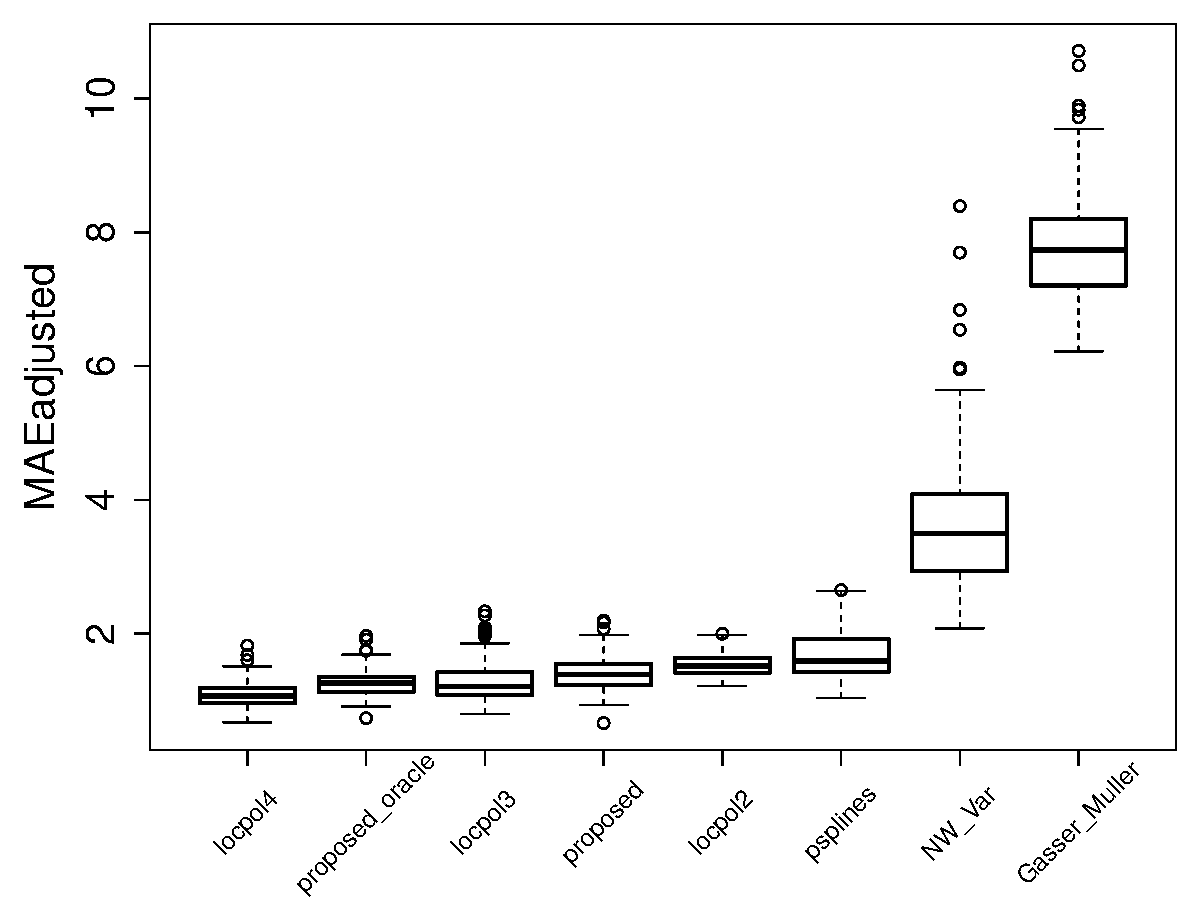
\includegraphics[width=1\linewidth]{Code/Figures/sim3_deriv_boxplot_full.pdf}
		\caption{Results for simulation study \eqref{sim3_eq}.}
	\end{subfigure}
	\hfil
	\begin{subfigure}[t]{0.49\linewidth}
		\centering
		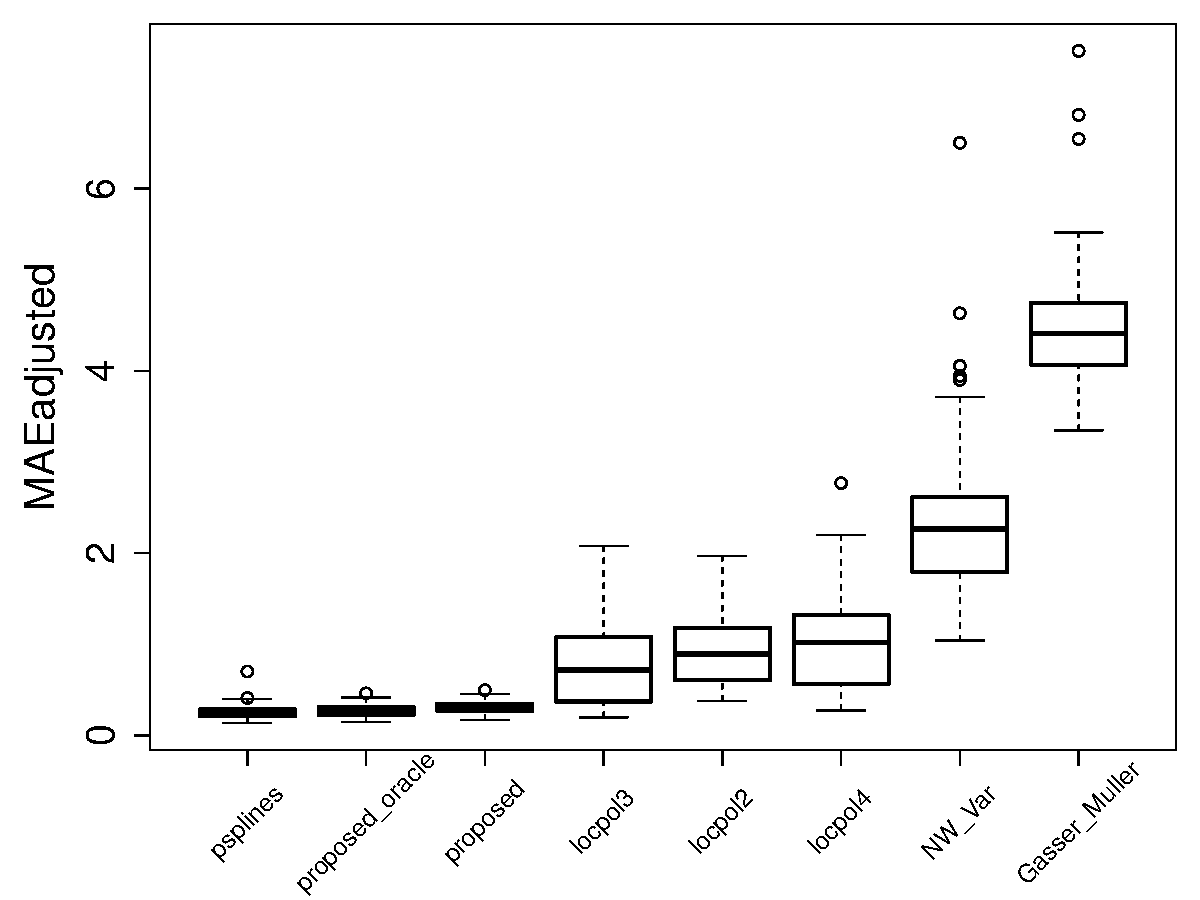
\includegraphics[width=1\linewidth]{Code/Figures/sim4_deriv_boxplot_full.pdf}
		\caption{Results for simulation study \eqref{sim4_eq}.}
	\end{subfigure}
	\caption{Comparative boxplots of the proposed first-order derivative estimator and all the methods that we compare under the Monte Carlo simulation studies \eqref{sim3_eq} and \eqref{sim4_eq}. We order the boxplots in each panel according to the increasing order of the average values of their adjusted MAEs. (This figure is extended from Figure 5 and Figure 6(b) in the paper.)}
	\label{fig:sim_first_boxplot}
\end{figure}

As in the discussed paper, we simulate data sets of size $n=700$ from model \eqref{rand_design} with the function
\begin{equation}
\label{sim3_eq}
m(X) = \sqrt{X(1-X)} \cdot\sin\left(\frac{2.1\pi}{X+0.05}\right) \quad \text{ with } \quad X\sim \mathrm{Unif}(0.25,1) \quad \text{ and } \quad e\sim N(0,0.2^2)
\end{equation}
for $100$ times. The tuning parameter $k$ is selected via Corollary~\ref{cor:k_sel} over the positive integer set $\left\{1,2,...,\floor{\frac{n-1}{2}}\right\}$ unless otherwise stated. The bandwidth $h$ of the proposed estimator \eqref{loc_poly_first} is initially selected from the set $\{0.03, 0.035,...,0.07\}$ through a local cubic regression with the bimodal Gaussian kernel and corrected for the unimodal Gaussian kernel as in Section~\ref{Sec:loc_poly}. The paper also considered another Monte Carlo simulation with a nonuniform distribution of $X$ under model \eqref{rand_design} as:
\begin{equation}
	\label{sim4_eq}
	m(X) = X+ 2\exp\left(-16X^2\right) \quad \text{ with } \quad X\sim N(0,0.5^2) \quad \text{ and } \quad e\sim N(0,0.2^2),
\end{equation}
where the sample size is again $n=700$ and the data generating process is repeated for 100 times. The initial bandwidth in this case is selected from the set $\{0.04, 0.045,...,0.08\}$ and corrected for a unimodal Gaussian kernel as well. We adopt the adjusted mean absolute error $\text{MAEadj}=\frac{1}{650}\sum_{i=26}^{675} \left|\hat{m}^{(1)}(X_{(i)}) -m^{(1)}(X_{(i)}) \right|$ without boundary points from the paper as an evaluation metric. Based on our offline experiments, this performance measure yields some similar comparative results to the scenarios when we use a more robust median absolute error metric. \autoref{fig:sim_first_boxplot} demonstrates that even with oracle knowledge about the distribution of covariate $X$, the proposed first-order derivative estimator is outperformed by local polynomial regression with $p=4$ or penalized smoothing cubic splines in the above simulation settings \eqref{sim3_eq} and \eqref{sim4_eq} from the discussed paper. The reason why we can discover the cases when the proposed first-order derivative estimation method is outperformed by classical methods is that our experiments are more comprehensive than those in the paper.


\subsection{Simulation Studies on the Second-Order Derivative Estimation}
\label{Sec:sim_second_order}

\begin{figure}
	\captionsetup[subfigure]{justification=centering}
	\begin{subfigure}[t]{0.49\linewidth}
		\centering
		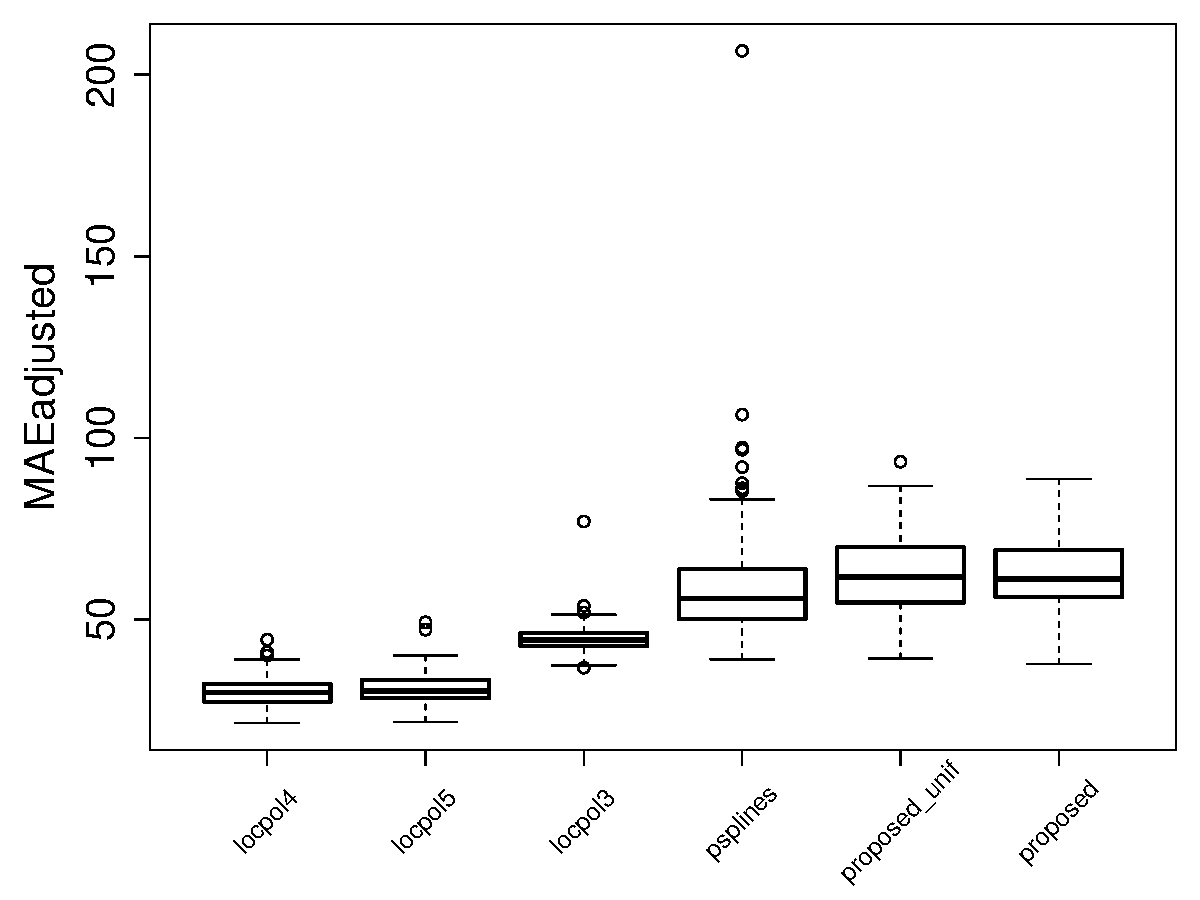
\includegraphics[width=1\linewidth]{Code/Figures/sim7_sec_boxplot_sub.pdf}
		\caption{Results for simulation study \eqref{sim7_eq}.}
	\end{subfigure}
	\hfil
	\begin{subfigure}[t]{0.49\linewidth}
		\centering
		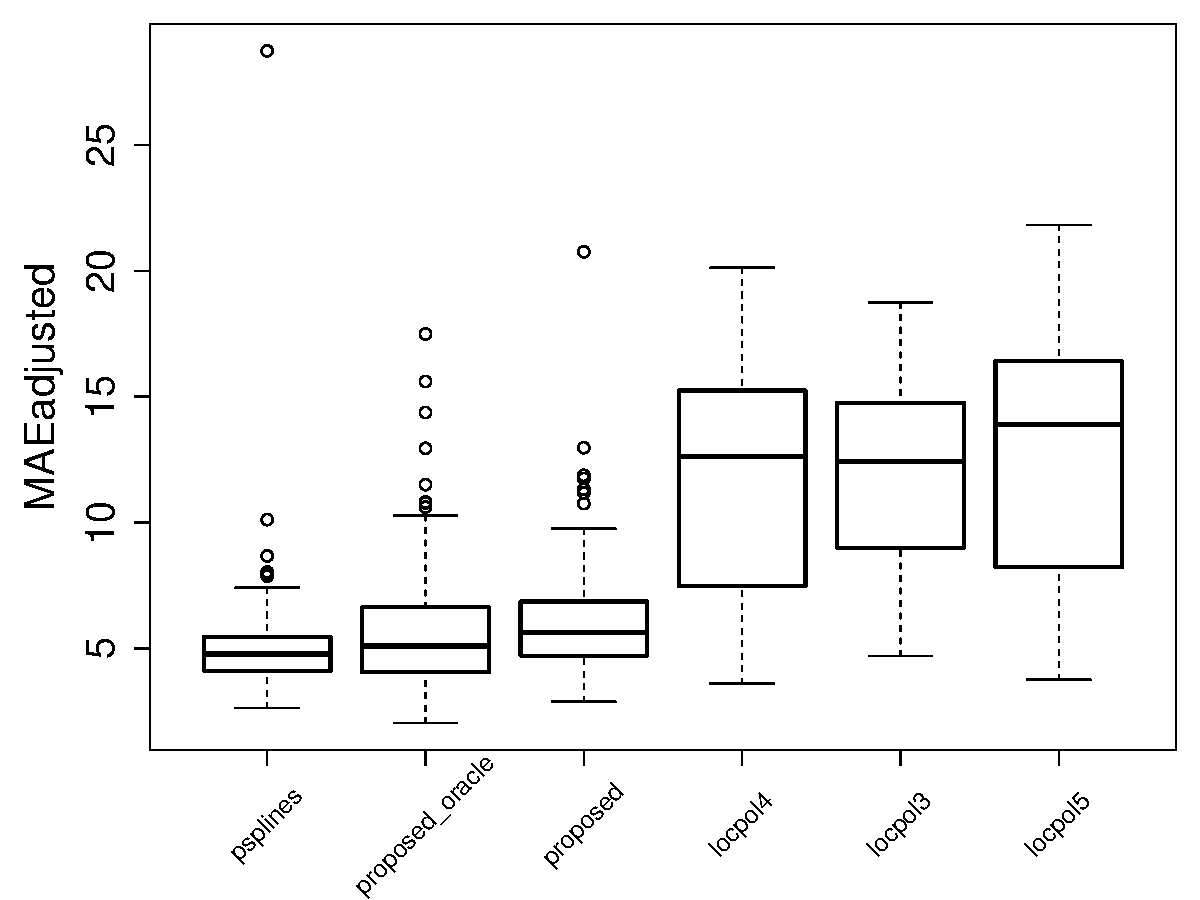
\includegraphics[width=1\linewidth]{Code/Figures/sim4_sec_boxplot_sub.pdf}
		\caption{Results for simulation study \eqref{sim4_eq}.}
	\end{subfigure}
	\caption{Comparative boxplots of the proposed second-order derivative estimator and the methods that we compare under the Monte Carlo simulation studies \eqref{sim7_eq} and \eqref{sim4_eq}. We order the boxplots in each panel according to the increasing order of the average values of their adjusted MAEs. (This figure is extended from Figure 11 and Figure 6(b) in the paper.)}
	\label{fig:sim_second_boxplot}
\end{figure}

As in the discussed paper, we simulate data sets of size $n=700$ from model \eqref{rand_design} with the function
\begin{equation}
\label{sim7_eq}
m(X) = 8e^{-(1-5X)^3(1-7X)} \quad \text{ with } \quad X\sim \mathrm{Unif}(0,1) \quad \text{ and } \quad e\sim N(0,0.1^2)
\end{equation}
for $100$ times. The tuning parameters $k_1,k_2$ are selected via Corollary~\ref{cor:k1_k2_sel} over the product integer set $\{1,...,100\} \otimes \{1,...,100\}$. The initial bandwidth $h$ of the proposed estimator \eqref{local_poly_second} is selected from the set $\{0.03, 0.035,...,0.1\}$ through a local cubic regression with the bimodal Gaussian kernel and then corrected for the unimodal Gaussian kernel as in Section~\ref{Sec:loc_poly}. Given that the paper did not consider the nonuniform distributional design of $X$, we make an extension here by reusing the Monte Carlo simulation study \eqref{sim4_eq} but estimating the second-order derivative of $m$. The performance measure is adopted from the paper as another adjusted mean absolute error $\text{MAEadj}=\frac{1}{640}\sum_{i=31}^{670} \left|\hat{m}^{(2)}(X_{(i)}) - m^{(2)}(X_{(i)}) \right|$. \autoref{fig:sim_second_boxplot} presents the comparative boxplots of various second-order derivative estimation methods under these two simulation studies, where we remove the results of Gasser-M\"uller and Nadaraya-Watson derivative estimators due to their inferior performances. Different from what the paper claimed, the proposed second-order derivative again behaves worse than the local polynomial regression of some certain order and penalized smoothing cubic splines.

% \subsection{Case Study: Washington State-Level COVID-19 Case Rates}

\section{Discussion}

The discussed paper \citep{liu2020smoothed} proposes a data-driven method for derivative estimation under the random design by combining the weighted difference quotients with local polynomial regression and studies the asymptotic properties of the proposed derivative estimators. While the proposed derivative estimation framework is not novel given the previous works \citep{de2013derivative,de2018local}, the theoretical analysis under the random design in the paper has its own merit, especially with our complementary results (\autoref{thm:conv_rate_full}). Nevertheless, our reproducing and extensive simulation studies demonstrate that the proposed first and second-order derivative estimators are outperformed by other classical derivative estimation methods under the simulation settings of the paper. Furthermore, we record the elapsed time for each derivative estimation method in the Monte Carlo simulation study \eqref{sim3_eq} in \autoref{fig:time_comp}, where the proposed method is less computationally efficient than other methods due to its time required to select tuning parameters.

\begin{wrapfigure}{r}{0.471\textwidth}
	\centering
	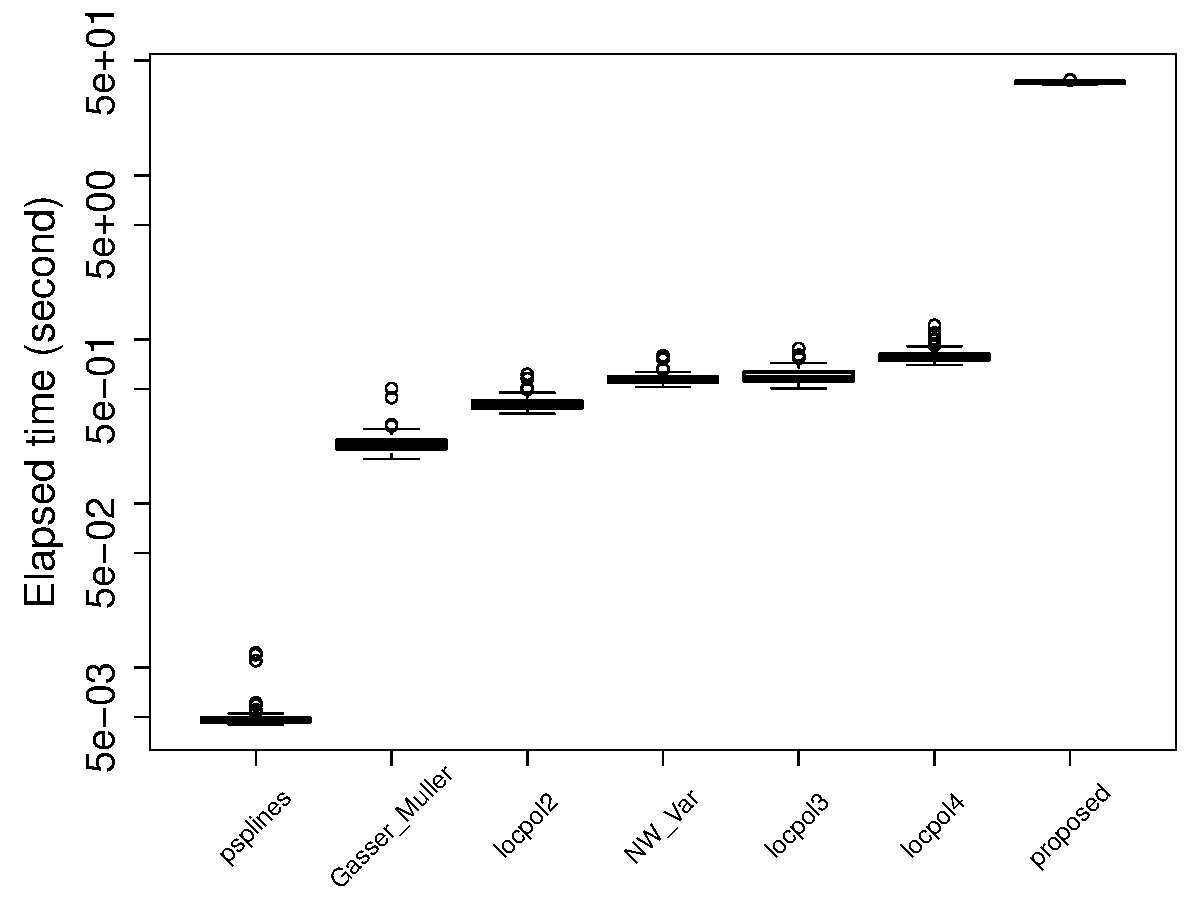
\includegraphics[width=1\linewidth]{Code/Figures/time_comp.pdf}
	\caption{Time comparisons of different first-order derivative estimation methods.}
	\label{fig:time_comp}
\end{wrapfigure}

One promising direction for improving the accuracy of the proposed method is to smooth the observed sample $\{(X_i,Y_i)\}_{i=1}^n$ first by penalized smoothing splines (see Simulation 8 in Appendix~\ref{App:poten_improve}) or local random forests \citep{dang2021smoothed,dang2022machine} before taking weighted difference quotients as noisy derivative estimators. Studying the asymptotic properties of such a pre-smoothed derivative estimator will be of research interest. In addition, while \cite{dang2021smoothed} already considered generalizing the proposed method to estimating (partial) derivatives of a multivariate regression function under the random design, a strong independence assumption between covariates in its multivariate probability integral transformation step was imposed. In general, when the covariates are dependent, it is not true that the CDF of the covariate vector $\bm{X}\in \mathbb{R}^d$ is uniformly distributed on $[0,1]$. Nor is it possible to reconstruct the distribution of $\bm{X}$ through its joint CDF \citep{genest2001multivariate}. To tackle this multivariate derivative estimation problem, one may resort to the associated copula \citep{nelsen2007introduction} in order to model the dependence structure between $\bm{X}$ and characterize its entire distribution.


\pagebreak

\section*{Acknowledgement}

I would like to thank Professor Thomas Richardson for his detailed and insightful comments on this report and my progress towards the preliminary exam throughout the entire quarter. I also acknowledge Professor Marina Meil\u{a}, Professor Yen-Chi Chen, Professor Alexander Giessing, Steven Wilkins-Reeves, Apara Venkat, and members of the Geometric Data Analysis reading group at the University of Washington for their comments and suggestions to my presentation.

\bibliography{Stat572Bib}

\appendix

\vspace{10mm}

\noindent{\bf Summary of the Appendix:}
\begin{itemize}
	\item Appendix~\ref{App:repro}: We reproduce all the simulation studies and figures in the discussed paper \citep{liu2020smoothed} and showcase a real-world application of the proposed first-order derivative estimation methods to Washington state-level COVID-19 case rates.
	
	\item Appendix~\ref{App:proofs}: We provide all the proofs of theorems and theoretical results in the main report.
\end{itemize}


\section{Other Reproducing Simulation Studies}
\label{App:repro}

This section presents all the simulation studies and figures in the paper \citep{liu2020smoothed} that have yet been discussed in Section~\ref{Sec:experiments} of the main report. Since the authors of the discussed paper did not make any code publicly available, I programmed the proposed derivative estimation methods as well as all the simulation studies by myself. Although the smoothed estimators $\hat{r}^{(1)}$ and $\hat{r}^{(2)}$ are constructed with noisy derivative data for interior points in \autoref{thm:loc_poly_first} and \autoref{thm:local_poly_second}, the paper also includes the noisy derivative data at the boundary to obtain these smoothed derivative estimators by the local polynomial regression in its simulation studies. \emph{I noticed that only including the interior noisy derivative data for the local polynomial regression as suggested by \autoref{thm:loc_poly_first} and \autoref{thm:local_poly_second} makes our reproducing figures look more similar to the original ones in the paper, and the proposed derivative estimation methods have lower estimation errors. Thus, we will use this strategy for our reproducing simulation studies in this report.} In addition, it is worth mentioning that exactly reproducing some figures without any knowledge about the random seeds for simulations is almost impossible, so there may be some tiny discrepancies between the original figures in the paper and the ones that I reproduce as follows.

\subsection{Simulation Studies on the First-Order Derivative Estimation}

For all the simulation studies in this section, the density $f$ and CDF $F$ of the covariate $X$ are estimated by the \texttt{R} functions \texttt{kde} and \texttt{kcde} with default parameters in the \texttt{R} package \texttt{ks} \citep{ks2022R}. The tuning parameter $k$ is selected via Corollary~\ref{cor:k_sel} over the positive integer set $\left\{1,2,...,\floor{\frac{n-1}{2}}\right\}$ unless otherwise stated. We apply the local cubic regression ($p=3$) with the bimodal kernel $\bar{K}(u)=\frac{2u^2}{\sqrt{\pi}} \exp\left(-u^2\right)$ to initially select the bandwidth parameter from a set and correct it for a unimodal Gaussian kernel $K(u)=\frac{1}{\sqrt{2\pi}} \exp\left(-\frac{u^2}{2}\right)$ as described in Section~\ref{Sec:loc_poly}.

\indent $\bullet$ {\bf Simulation 1:} The first simulation study in the paper \citep{liu2020smoothed} has been presented in \autoref{fig:sim1} of the main report, in which the simulated observations $\{(X_i,Y_i)\}_{i=1}^n$ with $n=1000$ is sampled from model \eqref{rand_design} with
\begin{equation}
\label{sim1_eq}
m(X) = \cos^2(2\pi X) + \log(4/3 +X) \quad \text{ for } \quad X\sim \mathrm{Unif}(0,1)
\end{equation}
and $e\sim N(0,0.1^2)$, whose true first-order derivative is $m^{(1)}(X)=-2\pi \sin(4\pi X) + \frac{3}{3X+4}$. The initial bandwidth for the proposed derivative estimator is selected from the set $\{0.04, 0.045,...,0.1\}$. We compare our reproducing figures with the original ones in the paper in \autoref{fig:sim1_rep} as well.

\begin{figure}[t]
	\captionsetup[subfigure]{justification=centering}
	\begin{subfigure}[t]{0.32\linewidth}
		\centering
		\includegraphics[width=1\linewidth]{Figures_Org/Fig1a.png}
		\caption{Figure 1(a) in the paper.}
	\end{subfigure}
	\hfil
	\begin{subfigure}[t]{0.32\linewidth}
		\centering
		\includegraphics[width=1\linewidth]{Figures_Org/Fig2a.png}
		\caption{Figure 2(a) in the paper.}
	\end{subfigure}
    \hfil
    \begin{subfigure}[t]{0.32\linewidth}
    	\centering
    	\includegraphics[width=1\linewidth]{Figures_Org/Fig2b.png}
    	\caption{Figure 2(b) in the paper.}
    \end{subfigure}
    \begin{subfigure}[t]{0.32\linewidth}
    	\centering
    	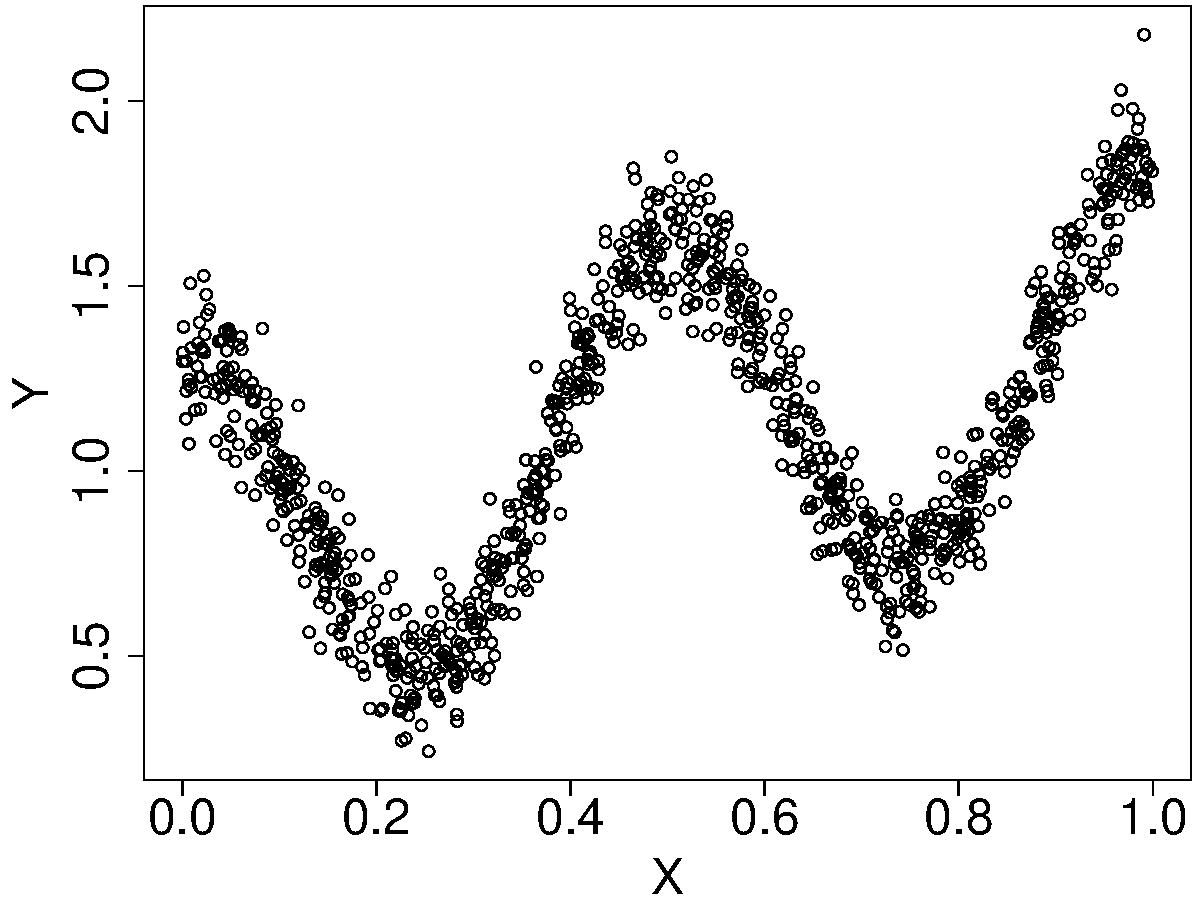
\includegraphics[width=1\linewidth]{Code/Figures/sim1_raw_rep.pdf}
    	\caption{Simulated observations.}
    \end{subfigure}
    \hfil
    \begin{subfigure}[t]{0.32\linewidth}
    	\centering
    	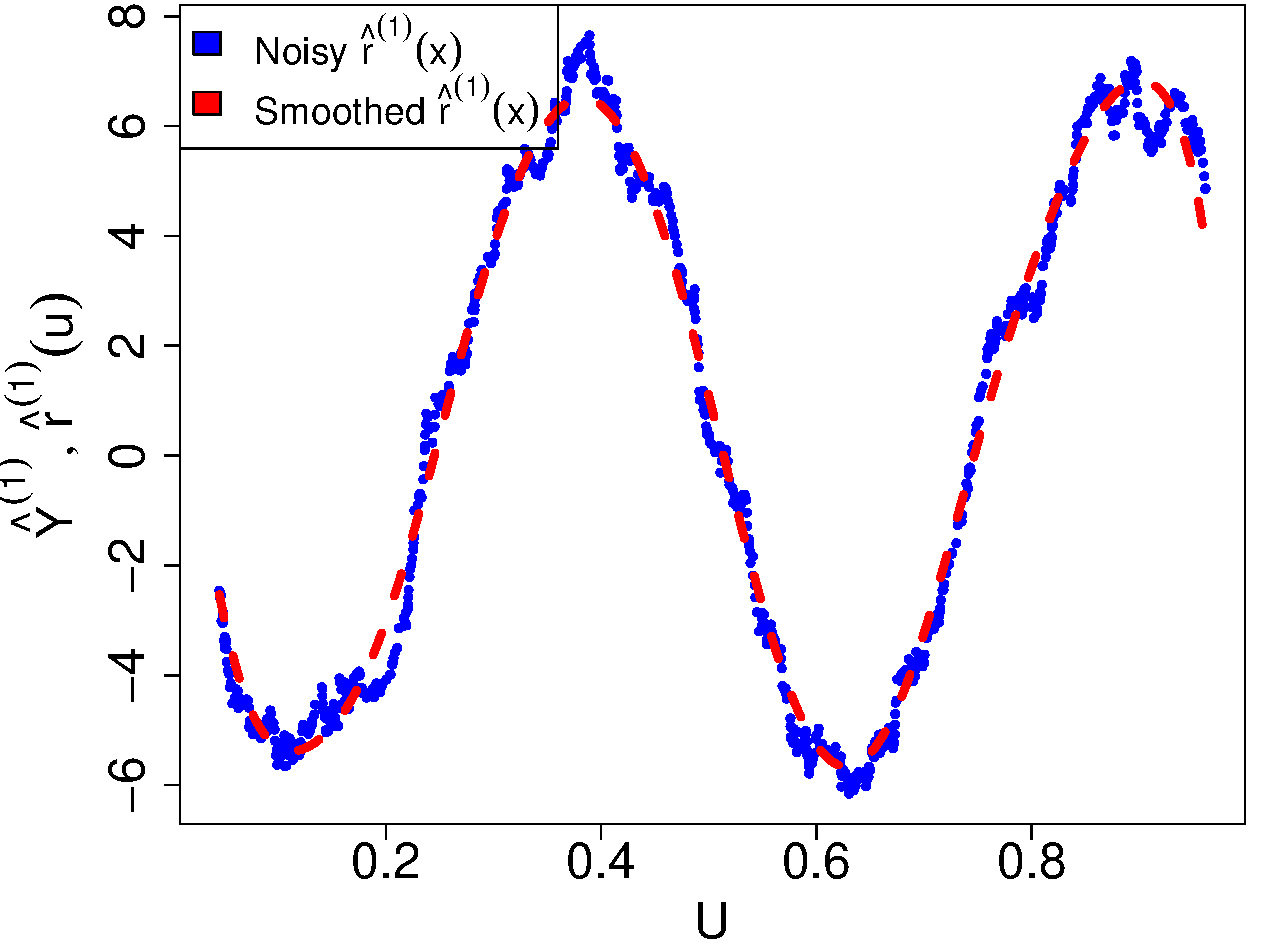
\includegraphics[width=1\linewidth]{Code/Figures/sim1_deriv_u.pdf}
    	\caption{First-order noisy derivatives with chosen $k=37$ and the smoothed estimates on the transformed space $[0,1]$.}
    \end{subfigure}
    \hfil
    \begin{subfigure}[t]{0.32\linewidth}
    	\centering
    	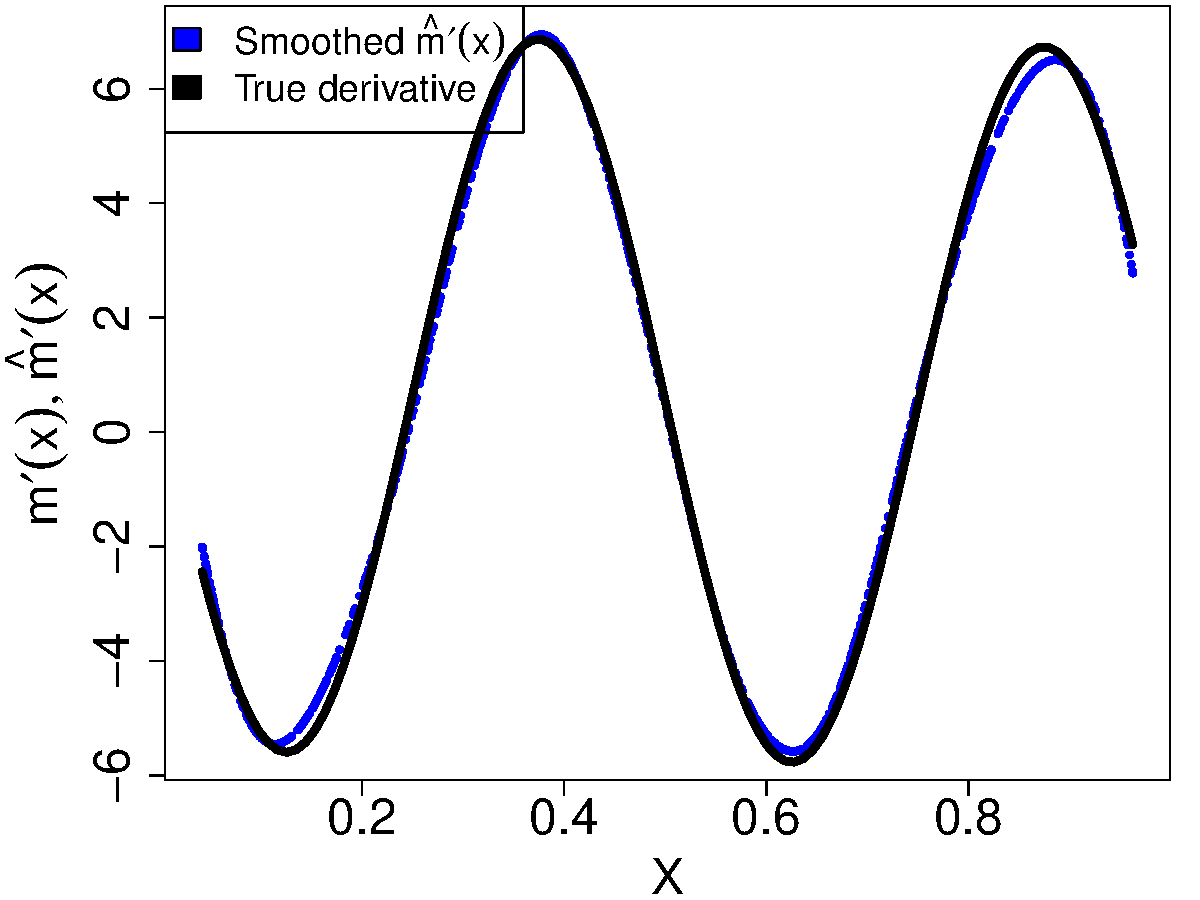
\includegraphics[width=1\linewidth]{Code/Figures/sim1_deriv_x_rep.pdf}
    	\caption{The proposed smoothed derivative estimates back-transformed to the original space with the true derivative.}
    \end{subfigure}
	\caption{{\bf Reproducing Figure 1(a) and Figure 2 in the paper:} Simulated data $\{(X_i,Y_i)\}_{i=1}^{1000}$ from model \eqref{rand_design} under \eqref{sim1_eq} with the first-order noisy derivatives and the proposed smoothed derivative estimates. The first row contains figures in the original paper, while the second row presents our reproduced figures.}
	\label{fig:sim1_rep}
\end{figure}


$\bullet$ {\bf Simulation 2:} The second simulation study in the paper \citep{liu2020smoothed} considers estimating the first-order derivative when the true distribution of $X$ is no longer uniform on $[0,1]$. In this case, the simulated observations $\{(X_i,Y_i)\}_{i=1}^n$ with $n=1000$ is sampled from model \eqref{rand_design} with
\begin{equation}
\label{sim2_eq}
m(X) = 50e^{-8(1-2X)^4} (1-2X)\quad \text{ for } \quad X\sim \mathrm{Beta}(2,2)
\end{equation}
and $e\sim N(0,2^2)$, whose true first-order derivative is $m^{(1)}(X) = 100\left[32(1-2X)^4 -1\right] e^{-8(1-2X)^4}$. The initial bandwidth for the proposed derivative estimator is selected from the set $\{0.04, 0.045,...,0.1\}$. We compare our reproducing figures with the original ones in the paper in \autoref{fig:sim2_rep}.

\begin{figure}[t]
	\captionsetup[subfigure]{justification=centering}
	\begin{subfigure}[t]{0.32\linewidth}
		\centering
		\includegraphics[width=1\linewidth]{Figures_Org/Fig1b.png}
		\caption{Figure 1(b) in the paper.}
	\end{subfigure}
	\hfil
	\begin{subfigure}[t]{0.32\linewidth}
		\centering
		\includegraphics[width=1\linewidth]{Figures_Org/Fig3a.png}
		\caption{Figure 3(a) in the paper.}
	\end{subfigure}
	\hfil
	\begin{subfigure}[t]{0.32\linewidth}
		\centering
		\includegraphics[width=1\linewidth]{Figures_Org/Fig3b.png}
		\caption{Figure 3(b) in the paper.}
	\end{subfigure}
	\begin{subfigure}[t]{0.32\linewidth}
		\centering
		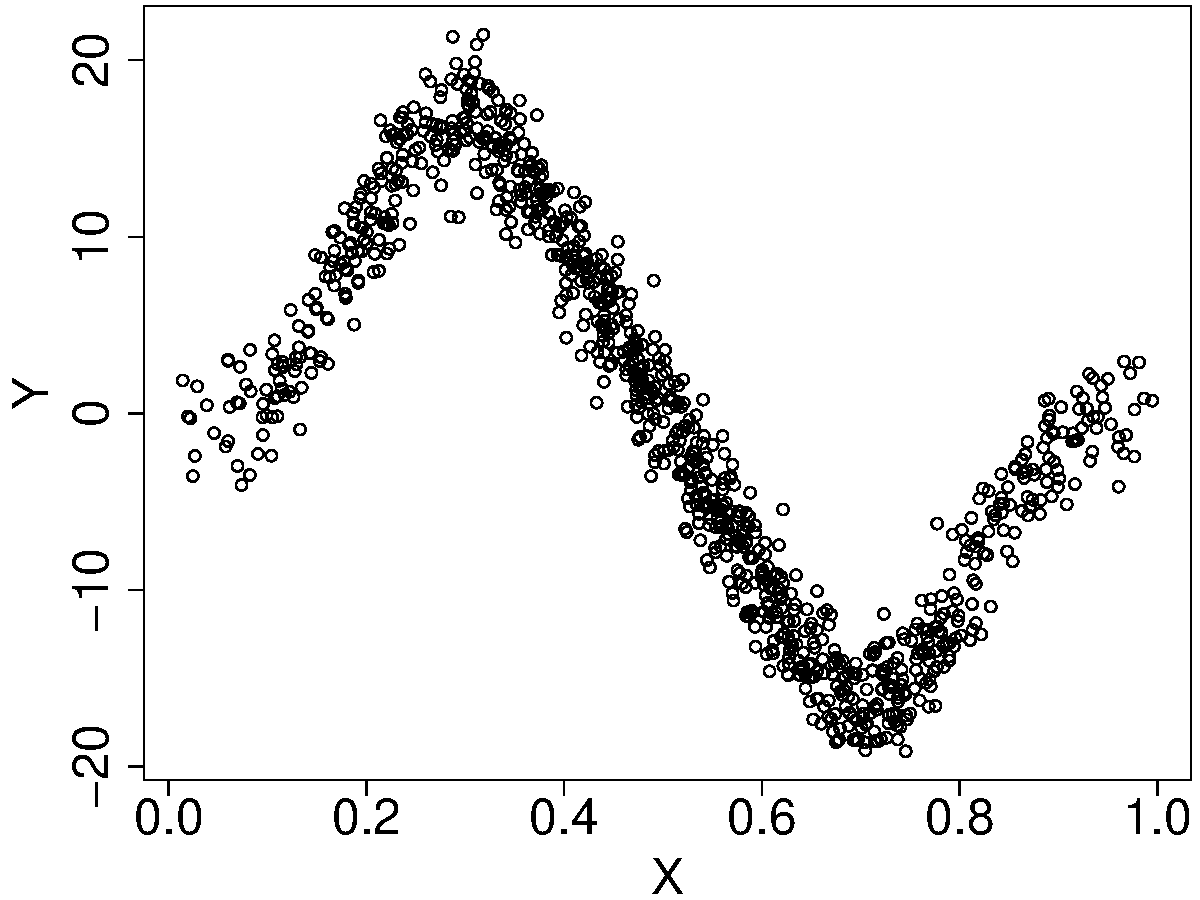
\includegraphics[width=1\linewidth]{Code/Figures/sim2_raw_rep.pdf}
		\caption{Simulated observations.}
	\end{subfigure}
	\hfil
	\begin{subfigure}[t]{0.32\linewidth}
		\centering
		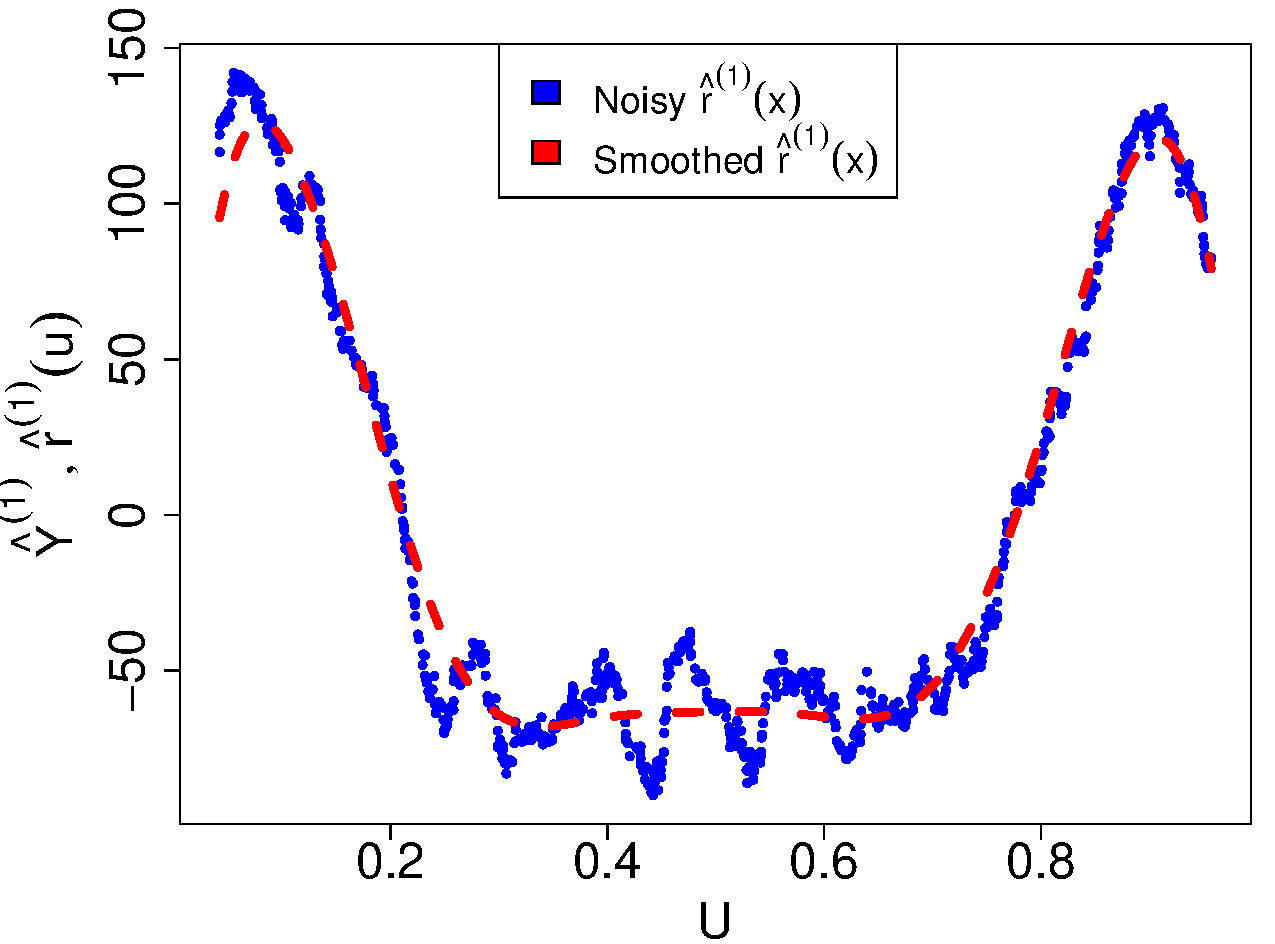
\includegraphics[width=1\linewidth]{Code/Figures/sim2_deriv_u.pdf}
		\caption{First-order noisy derivatives with chosen $k=39$ and the smoothed estimates on the transformed space $[0,1]$.}
	\end{subfigure}
	\hfil
	\begin{subfigure}[t]{0.32\linewidth}
		\centering
		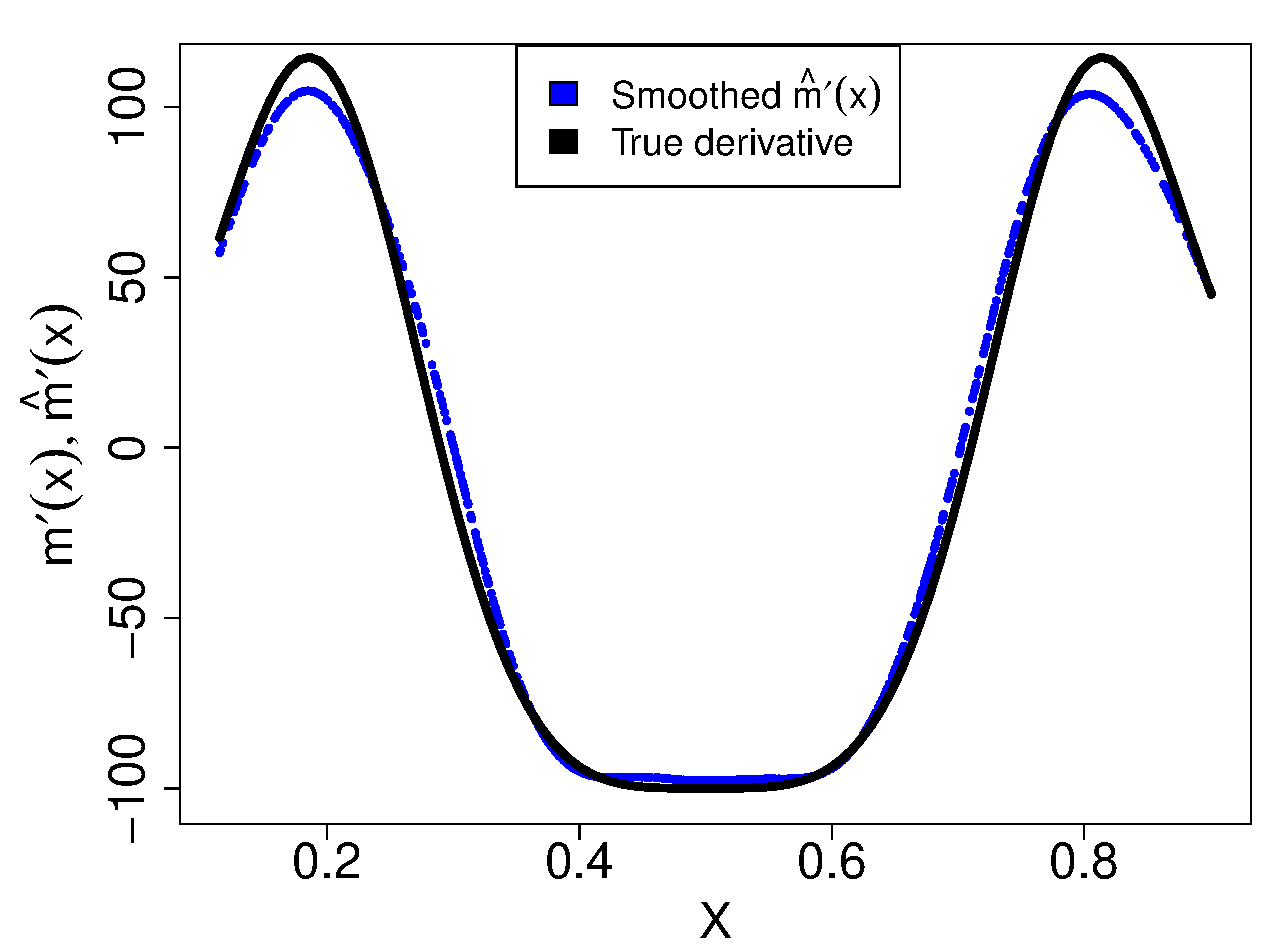
\includegraphics[width=1\linewidth]{Code/Figures/sim2_deriv_x_rep.pdf}
		\caption{The proposed smoothed derivative estimates back-transformed to the original space with the true derivative.}
	\end{subfigure}
	\caption{{\bf Reproducing Figure 1(b) and Figure 3 in the paper:} Simulated data $\{(X_i,Y_i)\}_{i=1}^{1000}$ from model \eqref{rand_design} under \eqref{sim2_eq} with the first-order noisy derivatives and the proposed smoothed derivative estimates. The first row contains figures in the original paper, while the second row presents our reproduced figures.}
	\label{fig:sim2_rep}
\end{figure}

$\bullet$ {\bf Simulation 3:} The third simulation study in the paper \citep{liu2020smoothed} is a Monte Carlo repeated simulation study described in \eqref{sim3_eq} of the main report, where the authors only compared the proposed first-order derivative estimator with the local slope of the local polynomial regression of order $p=2$ that is implemented in \texttt{R} package \texttt{locpol} \citep{locpol2022R} and the first-order derivative of the penalized smoothing cubic spline that is implemented in \texttt{R} package \texttt{pspline} \citep{pspline2022R}. The tuning parameter $k$ is chosen via Corollary~\ref{cor:k_sel} and the initial bandwidth is selected from the set $\{0.03, 0.035,...,0.07\}$ for each Monte Carlo simulated data set. In order to alleviate the boundary effects, the paper used an adjusted mean absolute error 
$$\text{MAEadj}=\frac{1}{650}\sum_{i=26}^{675} \left|\hat{m}^{(1)}(X_{(i)}) -m^{(1)}(X_{(i)}) \right|$$
as an evaluation metric. We compare our reproducing figures with the original ones in the paper in \autoref{fig:sim3_rep}, in which we also consider plugging in the true density $f$ and CDF $F$ in the probability integral transform step of the proposed estimator to illuminate the loss of accuracy due to the estimation of $f$ and $F$ in \autoref{fig:sim3_rep}(c,f).

\begin{figure}[!t]
	\captionsetup[subfigure]{justification=centering}
	\begin{subfigure}[t]{0.32\linewidth}
		\centering
		\includegraphics[width=1\linewidth]{Figures_Org/Fig4a.png}
		\caption{Figure 4(a) in the paper.}
	\end{subfigure}
	\hfil
	\begin{subfigure}[t]{0.32\linewidth}
		\centering
		\includegraphics[width=1\linewidth]{Figures_Org/Fig4b.png}
		\caption{Figure 4(b) in the paper.}
	\end{subfigure}
	\hfil
	\begin{subfigure}[t]{0.32\linewidth}
		\centering
		\includegraphics[width=1\linewidth,height=4.2cm]{Figures_Org/Fig5.png}
		\caption{Figure 5 in the paper.}
	\end{subfigure}
	\begin{subfigure}[t]{0.32\linewidth}
		\centering
		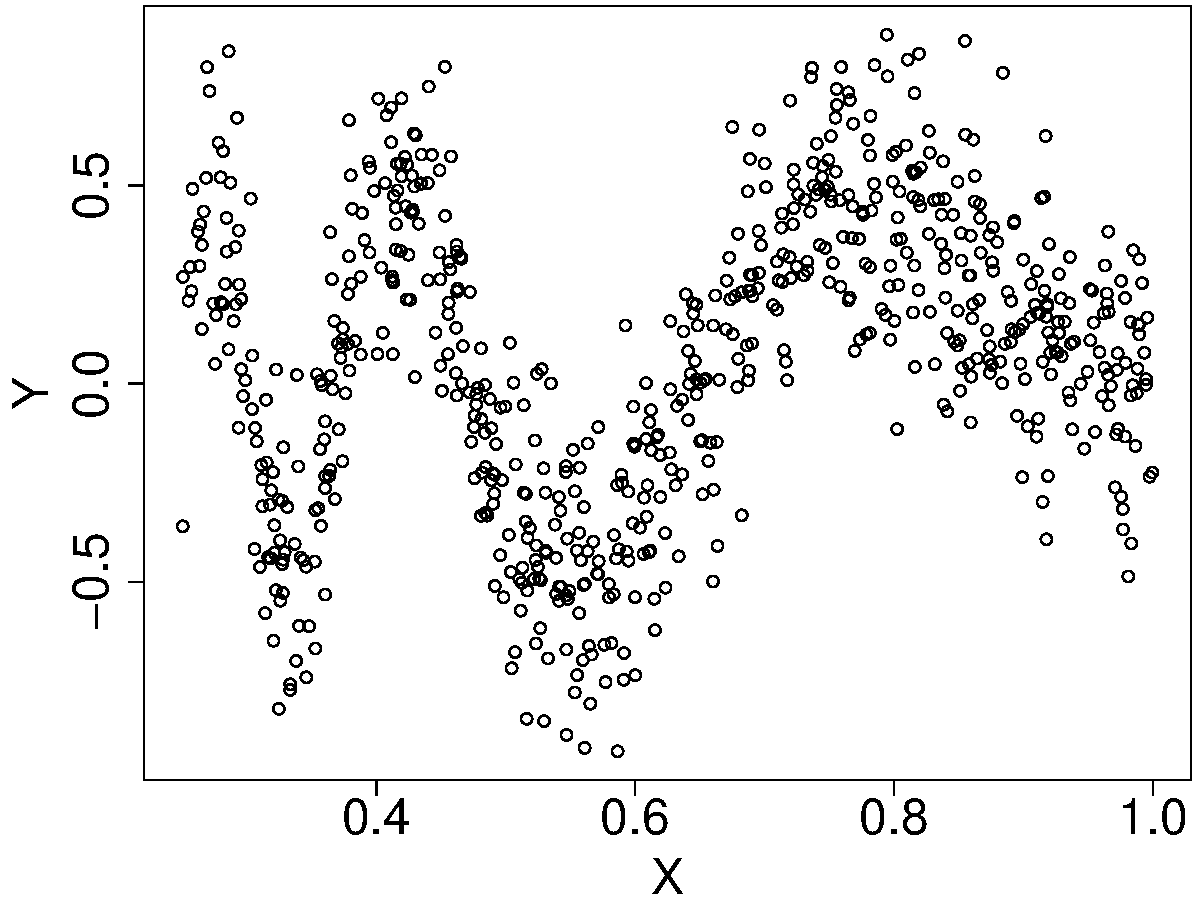
\includegraphics[width=1\linewidth]{Code/Figures/sim3_raw_rep.pdf}
		\caption{Simulated observations from one random run of model \eqref{sim3_eq}.}
	\end{subfigure}
	\hfil
	\begin{subfigure}[t]{0.32\linewidth}
		\centering
		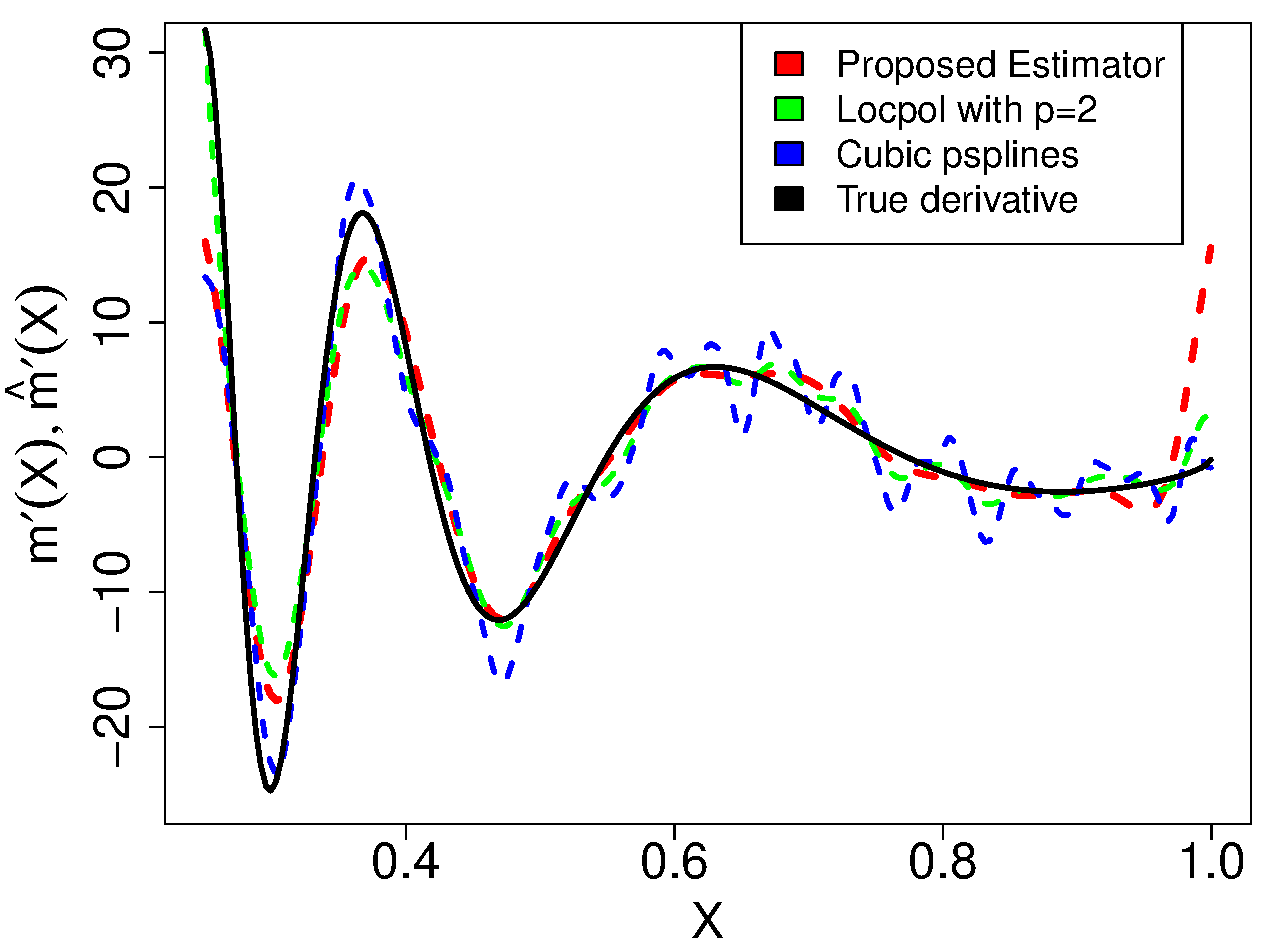
\includegraphics[width=1\linewidth]{Code/Figures/sim3_deriv_com.pdf}
		\caption{Proposed derivative estimator with chosen $k=10$, ``locpol2'', ``psplines'', and the true derivative.}
	\end{subfigure}
	\hfil
	\begin{subfigure}[t]{0.32\linewidth}
		\centering
		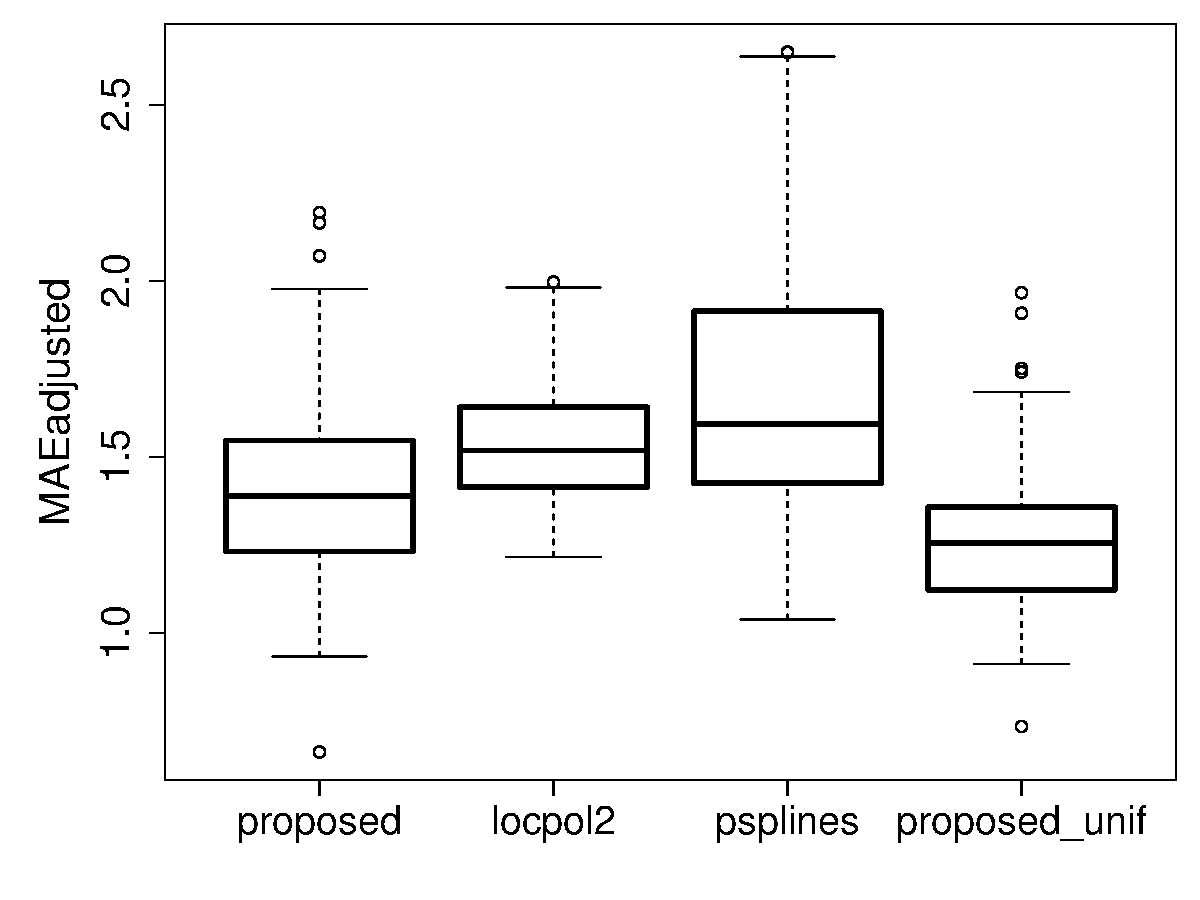
\includegraphics[width=1\linewidth]{Code/Figures/sim3_deriv_boxplot.pdf}
		\caption{Adjusted mean absolute errors under 100 Monte Carlo repeated experiments.}
	\end{subfigure}
	\caption{{\bf Reproducing Figures 4 and 5 in the paper:} Monte Carlo comparative studies from model \eqref{rand_design} under \eqref{sim3_eq} for the proposed first-order derivative estimator (``proposed''), the proposed first-order derivative estimator under the oracle distribution of $X$ (``proposed\_unif''), local polynomial regression estimator with $p=2$ (``locpol2''), and penalized smoothing cubic spline estimator (``psplines''). The first row contains figures in the original paper, while the second row presents our reproduced figures.}
	\label{fig:sim3_rep}
\end{figure}

$\bullet$ {\bf Simulation 4:} The fourth simulation study in the paper \citep{liu2020smoothed} is another Monte Carlo repeated simulation study described in \eqref{sim4_eq} of the main report, where the covariate $X$ is no longer uniformly distributed. Again, the authors only compared the proposed first-order derivative estimator with the local slope of the local polynomial regression of order $p=2$ and the first-order derivative of the penalized smoothing cubic spline with respect to the adjusted mean absolute error. The initial bandwidth for the proposed derivative estimator is selected from the set $\{0.04, 0.045,...,0.08\}$. We compare our reproducing figures with the original ones in the paper in \autoref{fig:sim4_rep}, in which we also consider plugging in the true density $f$ and CDF $F$ in the probability integral transform step of the proposed estimator to illuminate the loss of accuracy due to the estimation of $f$ and $F$ in \autoref{fig:sim4_rep}(b,d).

\begin{figure}[!t]
	\captionsetup[subfigure]{justification=centering}
	\begin{subfigure}[t]{0.49\linewidth}
		\centering
		\includegraphics[width=1\linewidth]{Figures_Org/Fig6a.png}
		\caption{Figure 6(a) in the paper.}
	\end{subfigure}
	\hfil
	\begin{subfigure}[t]{0.49\linewidth}
		\centering
		\includegraphics[width=1\linewidth,height=6cm]{Figures_Org/Fig6b.png}
		\caption{Figure 6(b) in the paper.}
	\end{subfigure}
	\begin{subfigure}[t]{0.49\linewidth}
		\centering
		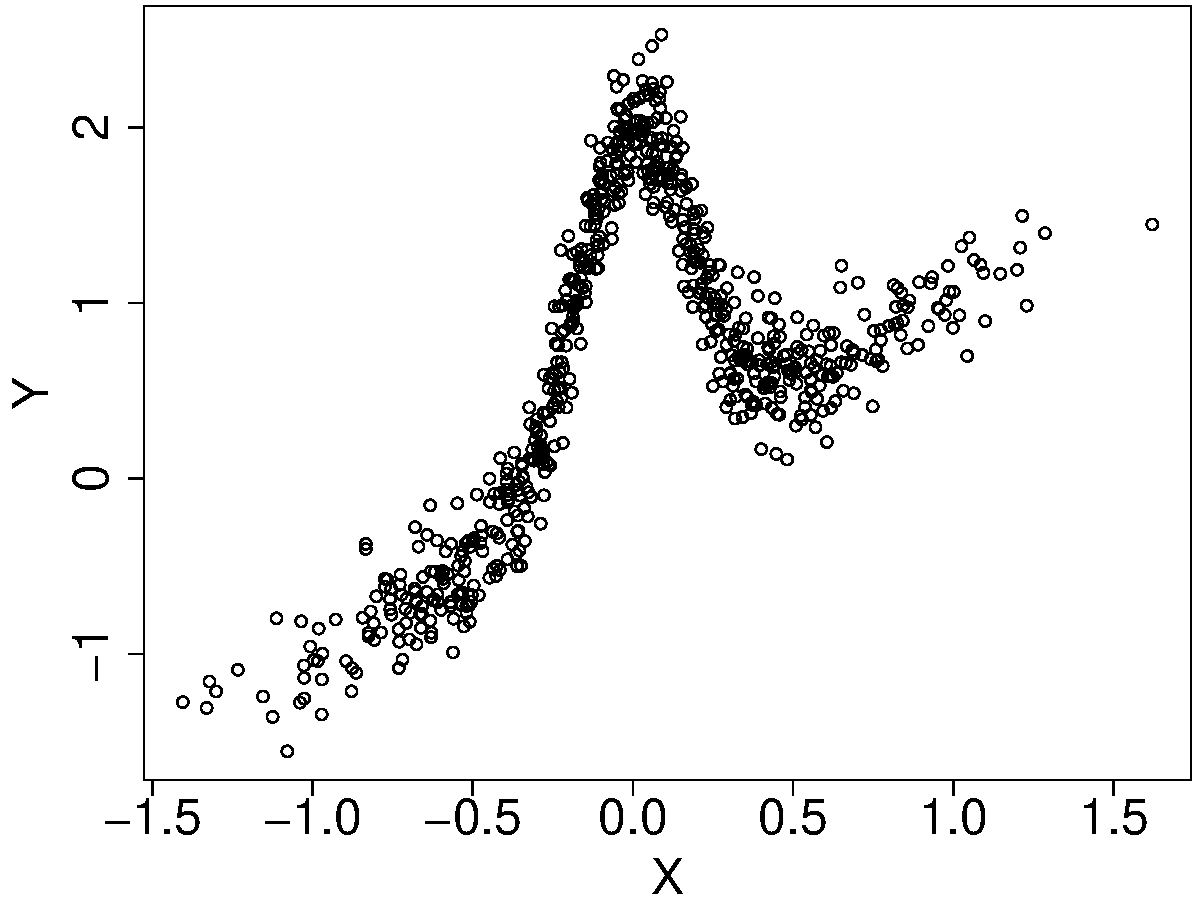
\includegraphics[width=1\linewidth]{Code/Figures/sim4_raw_rep.pdf}
		\caption{Simulation observations from one random run of model \eqref{sim4_eq}.}
	\end{subfigure}
	\hfil
	\begin{subfigure}[t]{0.49\linewidth}
		\centering
		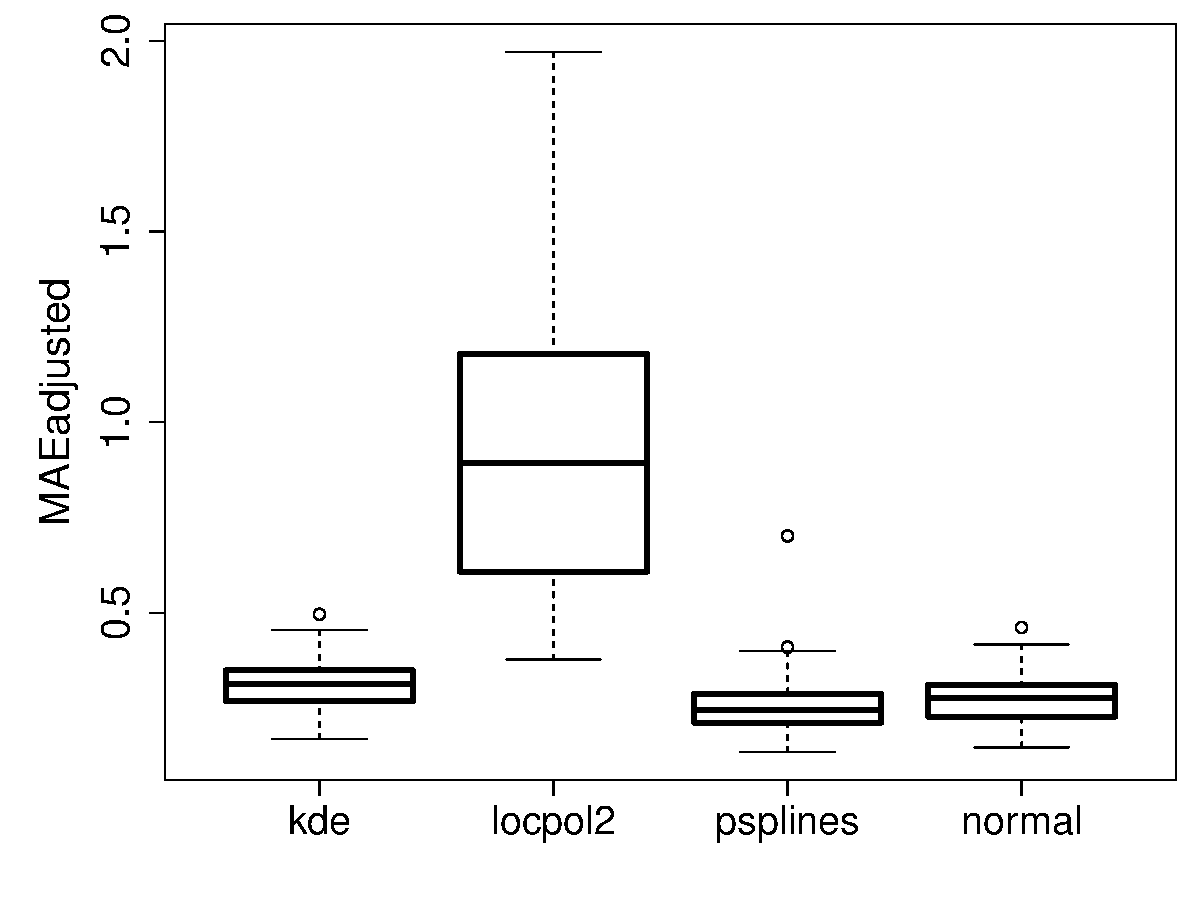
\includegraphics[width=1\linewidth]{Code/Figures/sim4_deriv_boxplot.pdf}
		\caption{Adjusted mean absolute errors under 100 Monte Carlo repeated experiments.}
	\end{subfigure}
	\caption{{\bf Reproducing Figure 6 in the paper:} Monte Carlo comparative studies from model \eqref{rand_design} under \eqref{sim4_eq} for the proposed first-order derivative estimator with KDE for the distribution of $X$ (``kde''), the proposed first-order derivative estimator under the oracle distribution of $X$ (``normal''), local polynomial regression estimator with $p=2$ (``locpol2''), and and penalized smoothing cubic spline estimator (``psplines''). The first row contains figures in the original paper, while the second row presents our reproduced figures.}
	\label{fig:sim4_rep}
\end{figure}

\subsection{Simulation Studies on the Second-Order Derivative Estimation}

Similar to the first-order derivative estimation, we estimate the density $f$, its derivative $f^{(1)}$, and CDF $F$ of the covariate $X$ through the \texttt{R} functions \texttt{kde}, \texttt{kdde}, and \texttt{kcde} with default parameters in the \texttt{R} package \texttt{ks} \citep{ks2022R}. The tuning parameters $k_1,k_2$ are selected via Corollary~\ref{cor:k1_k2_sel} over a product set of positive integers $\left\{1,2,...,100\right\}\otimes \left\{1,2,...,100\right\}$ unless otherwise stated. We apply the local cubic regression ($p=3$) with the bimodal kernel $\bar{K}(u)=\frac{2u^2}{\sqrt{\pi}} \exp\left(-u^2\right)$ to initially select the bandwidth parameter from a set and correct it for a unimodal Gaussian kernel $K(u)=\frac{1}{\sqrt{2\pi}} \exp\left(-\frac{u^2}{2}\right)$ as described in Section~\ref{Sec:loc_poly}.

$\bullet$ {\bf Simulation 5:} The fifth simulation study in the paper \citep{liu2020smoothed} reuses the data-generating mechanism of \eqref{sim1_eq} so that the true second-order derivative is $m^{(2)}(X) = -8\pi^2 \cos\left(4\pi X\right) - \frac{9}{(3X+4)^2}$. The initial bandwidth for the proposed derivative estimator is selected from the set $\{0.05, 0.055,...,0.1\}$. We compare our reproducing figures with the original ones in the paper in \autoref{fig:sim5_rep}.

\begin{figure}[!t]
	\captionsetup[subfigure]{justification=centering}
	\begin{subfigure}[t]{0.32\linewidth}
		\centering
		\includegraphics[width=1\linewidth]{Figures_Org/Fig7a.png}
		\caption{Figure 7(a) in the paper.}
	\end{subfigure}
	\hfil
	\begin{subfigure}[t]{0.32\linewidth}
		\centering
		\includegraphics[width=1\linewidth]{Figures_Org/Fig8a.png}
		\caption{Figure 8(a) in the paper.}
	\end{subfigure}
	\hfil
	\begin{subfigure}[t]{0.32\linewidth}
		\centering
		\includegraphics[width=1\linewidth]{Figures_Org/Fig9a.png}
		\caption{Figure 9(a) in the paper.}
	\end{subfigure}
	\begin{subfigure}[t]{0.32\linewidth}
		\centering
		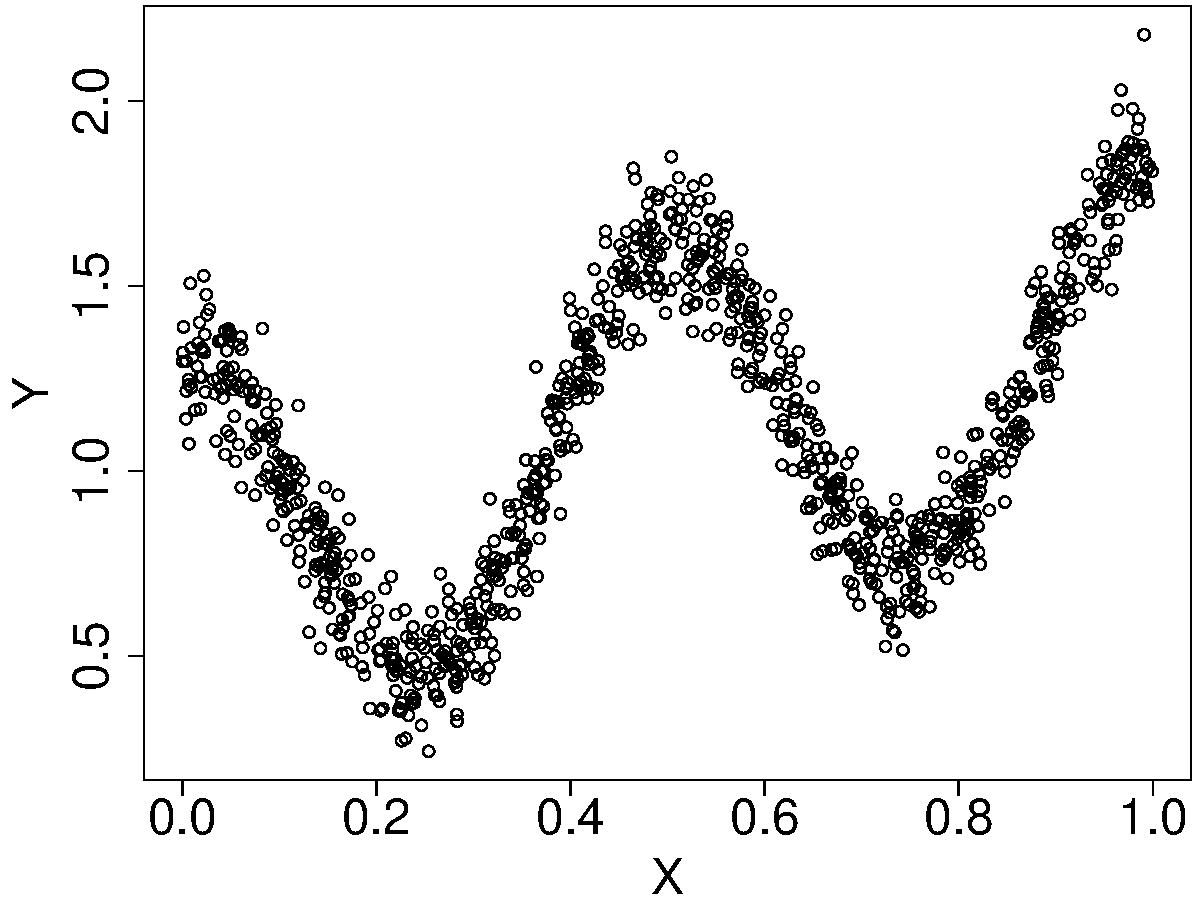
\includegraphics[width=1\linewidth]{Code/Figures/sim1_raw_rep.pdf}
		\caption{Simulated observations.}
	\end{subfigure}
	\hfil
	\begin{subfigure}[t]{0.32\linewidth}
		\centering
		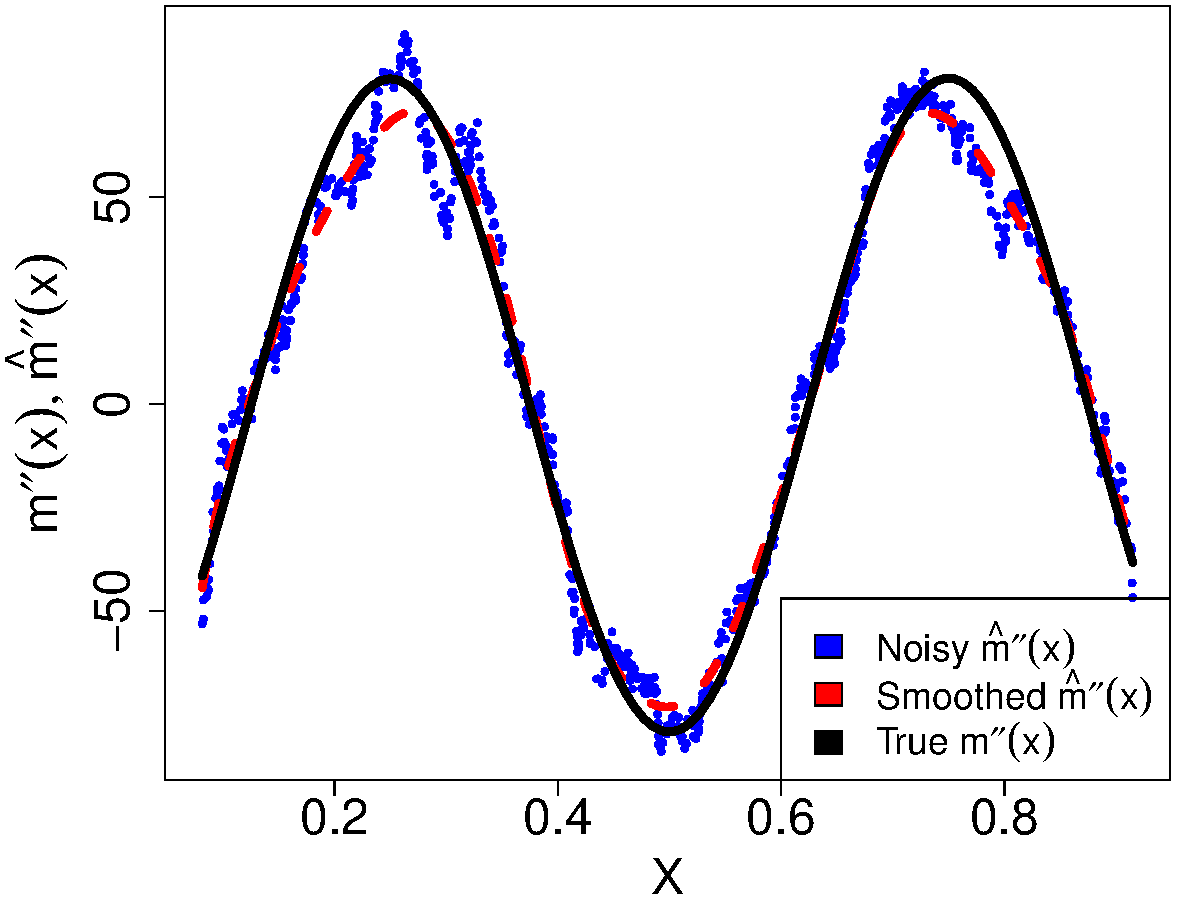
\includegraphics[width=1\linewidth]{Code/Figures/sim5_deriv.pdf}
		\caption{Second-order noisy derivatives with chosen $k_1=32, k_2=46$, the smoothed estimates, and the true derivative.}
	\end{subfigure}
	\hfil
	\begin{subfigure}[t]{0.32\linewidth}
		\centering
		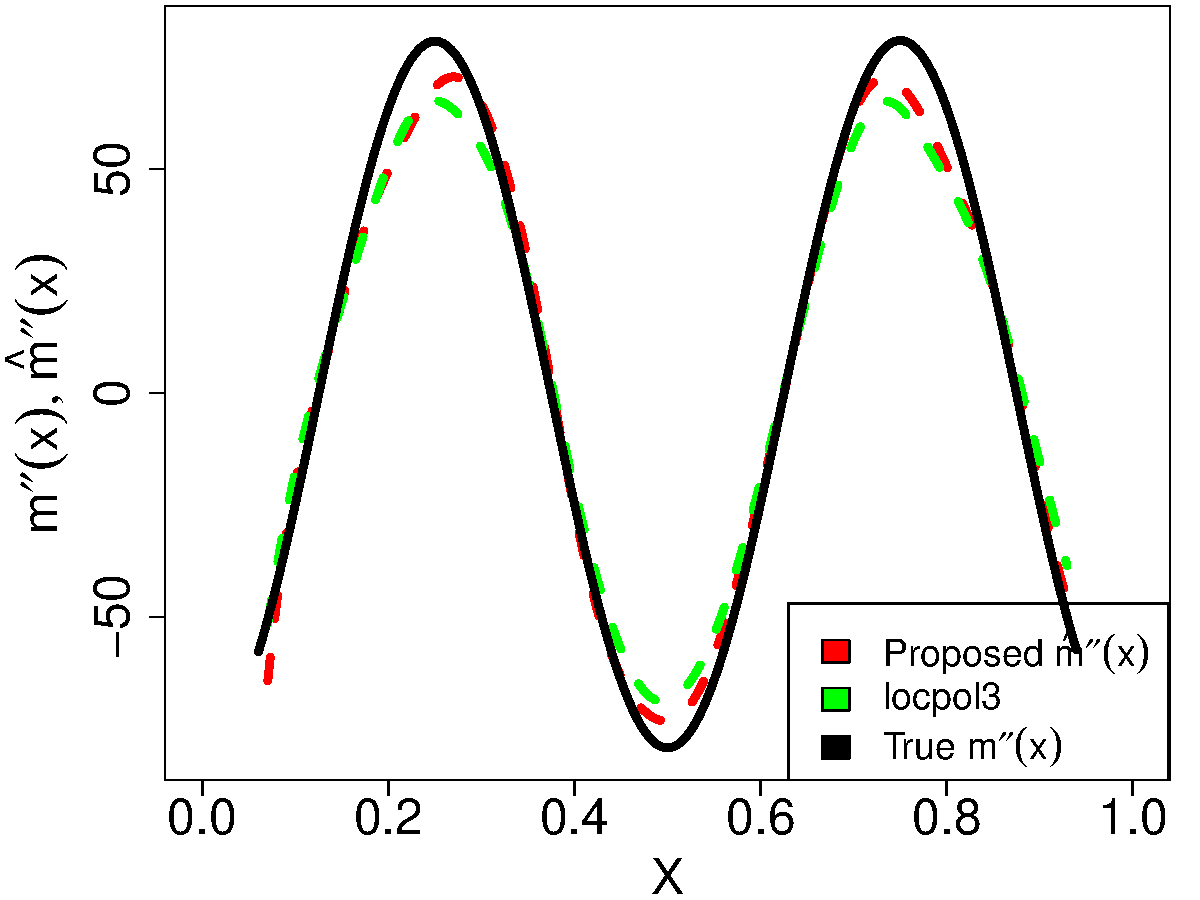
\includegraphics[width=1\linewidth]{Code/Figures/sim5_deriv_com.pdf}
		\caption{The proposed smoothed derivative estimates and the derivative of the local polynomial regression with $p=3$.}
	\end{subfigure}
	\caption{{\bf Reproducing Figure 7(a), Figure 8(a), and Figure 9(a) in the paper:} Simulated data $\{(X_i,Y_i)\}_{i=1}^{1000}$ from model \eqref{rand_design} under \eqref{sim1_eq} with the second-order noisy derivatives, the proposed smoothed derivative estimates, and their comparisons with the local polynomial regression estimator with $p=3$. The first row contains figures in the original paper, while the second row presents our reproduced figures.}
	\label{fig:sim5_rep}
\end{figure}


$\bullet$ {\bf Simulation 6:} The sixth simulation study in the paper \citep{liu2020smoothed} generates $n=1000$ observations $\{(X_i,Y_i)\}_{i=1}^n$ from model \eqref{rand_design} with the function
\begin{equation}
\label{sim6_eq}
m(X) = 50e^{-8(1-2X)^4} (1-2X)\quad \text{ for } \quad X\sim \mathrm{Unif}[0,1] \quad \text{ and } \quad e\sim N(0,2^2),
\end{equation}
whose true second-order derivative is $m^{(2)}(X)=6400(1-2X)^3\left[32(1-2X)^3 -5\right] e^{-8(1-2X)^4}$. The initial bandwidth for the proposed derivative estimator is again selected from the set $\{0.05, 0.055,...,0.1\}$. We compare our reproducing figures with the original ones in the paper in \autoref{fig:sim6_rep}.

\begin{figure}[!t]
	\captionsetup[subfigure]{justification=centering}
	\begin{subfigure}[t]{0.32\linewidth}
		\centering
		\includegraphics[width=1\linewidth]{Figures_Org/Fig7b.png}
		\caption{Figure 7(b) in the paper.}
	\end{subfigure}
	\hfil
	\begin{subfigure}[t]{0.32\linewidth}
		\centering
		\includegraphics[width=1\linewidth]{Figures_Org/Fig8b.png}
		\caption{Figure 8(b) in the paper.}
	\end{subfigure}
	\hfil
	\begin{subfigure}[t]{0.32\linewidth}
		\centering
		\includegraphics[width=1\linewidth]{Figures_Org/Fig9b.png}
		\caption{Figure 9(b) in the paper.}
	\end{subfigure}
	\begin{subfigure}[t]{0.32\linewidth}
		\centering
		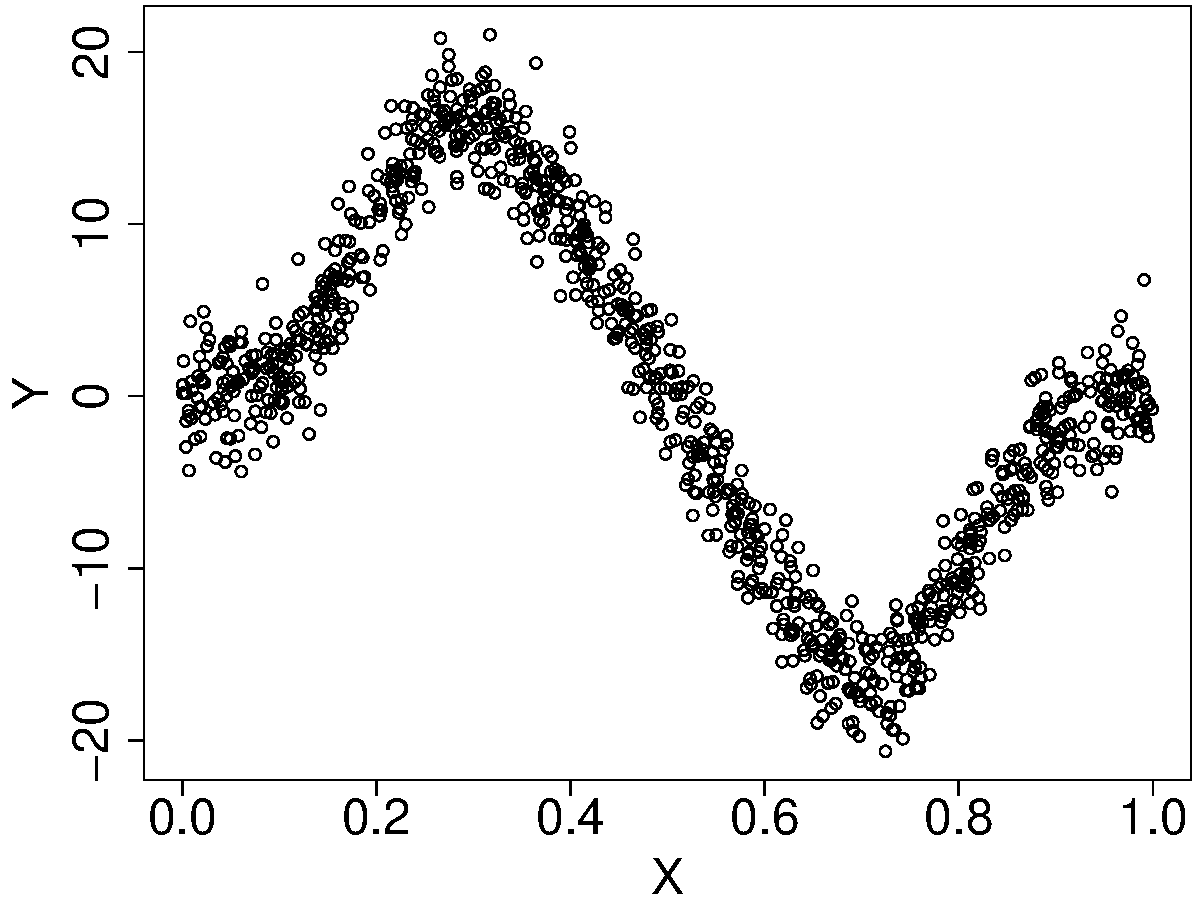
\includegraphics[width=1\linewidth]{Code/Figures/sim6_raw_rep.pdf}
		\caption{Simulated observations.}
	\end{subfigure}
	\hfil
	\begin{subfigure}[t]{0.32\linewidth}
		\centering
		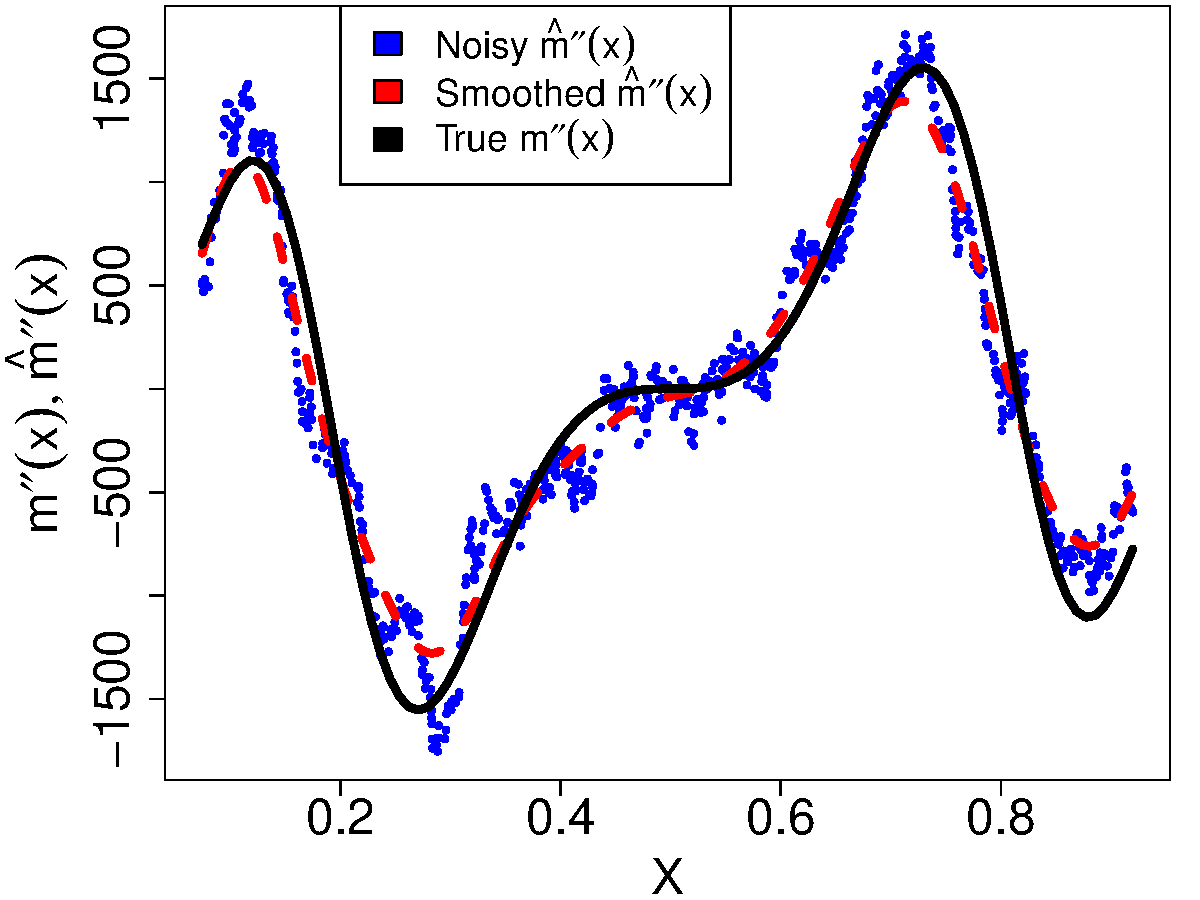
\includegraphics[width=1\linewidth]{Code/Figures/sim6_deriv.pdf}
		\caption{Second-order noisy derivatives with chosen $k_1=30, k_2=42$, the smoothed estimates, and the true derivative.}
	\end{subfigure}
	\hfil
	\begin{subfigure}[t]{0.32\linewidth}
		\centering
		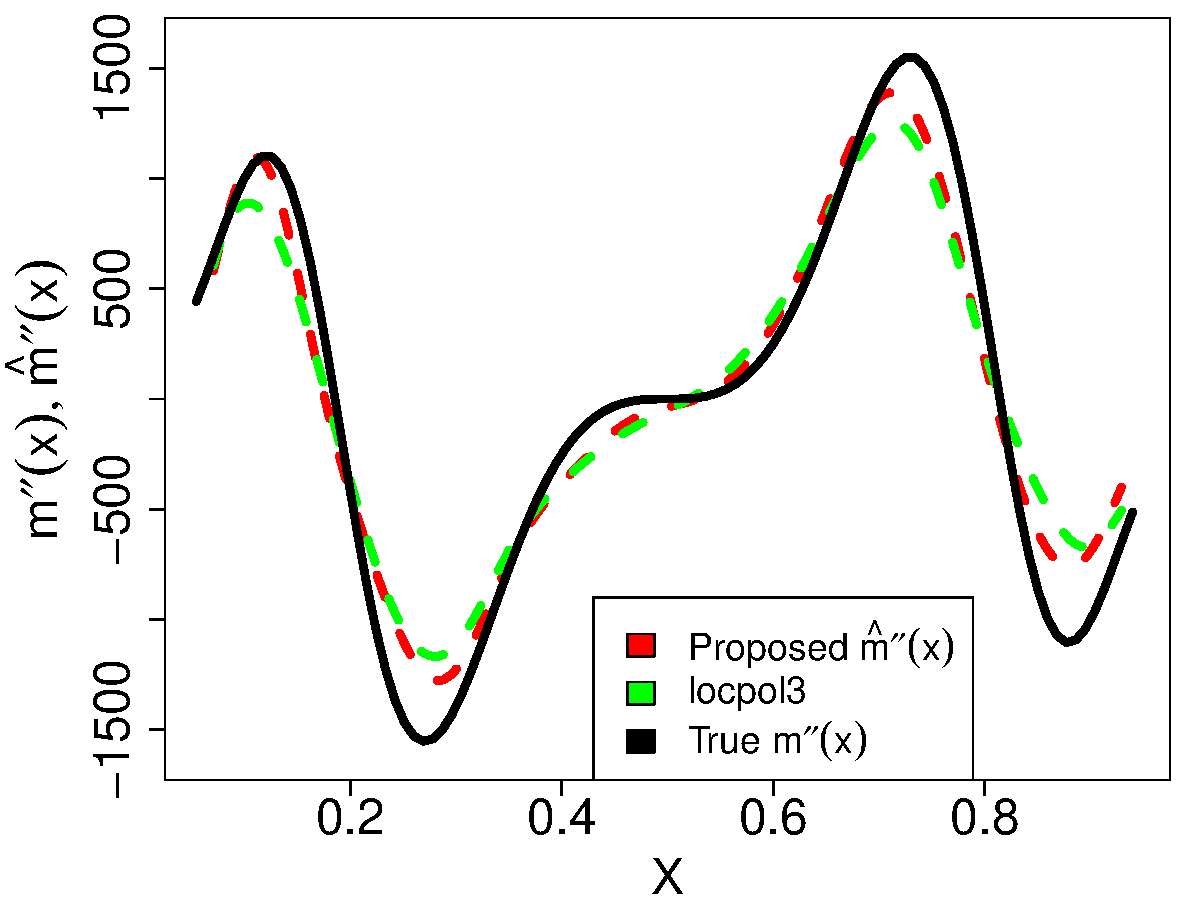
\includegraphics[width=1\linewidth]{Code/Figures/sim6_deriv_com.pdf}
		\caption{The proposed smoothed derivative estimates and the derivative of the local polynomial regression with $p=3$.}
	\end{subfigure}
	\caption{{\bf Reproducing Figure 7(b), Figure 8(b), and Figure 9(b) in the paper:} Simulated data $\{(X_i,Y_i)\}_{i=1}^{1000}$ from model \eqref{rand_design} under \eqref{sim6_eq} with the second-order noisy derivatives, the proposed smoothed derivative estimates, and their comparisons with the local polynomial regression estimator with $p=3$. The first row contains figures in the original paper, while the second row presents our reproduced figures.}
	\label{fig:sim6_rep}
\end{figure}

$\bullet$ {\bf Simulation 7:} The seventh simulation study in the paper \citep{liu2020smoothed} is a Monte Carlo repeated simulation study described in \eqref{sim7_eq}, where the authors only compared the proposed second-order derivative estimator with the local slope of the local polynomial regression of order $p=3$ implemented in \texttt{R} package \texttt{locpol} \citep{locpol2022R} and the second-order derivative of the penalized smoothing cubic spline implemented in \texttt{R} package \texttt{pspline} \citep{pspline2022R}. The tuning parameters $k_1,k_2$ are chosen via Corollary~\ref{cor:k1_k2_sel} and the initial bandwidth is selected from the set $\{0.03, 0.035,...,0.1\}$ for each Monte Carlo simulated data set. In order to alleviate the boundary effects, the paper again used an adjusted mean absolute error 
$$\text{MAEadj}=\frac{1}{640}\sum_{i=31}^{670} \left|\hat{m}^{(2)}(X_{(i)}) -m^{(2)}(X_{(i)}) \right|$$
as an evaluation metric. We compare our reproducing figures with the original ones in the paper in \autoref{fig:sim7_rep}. Notice that there are some discrepancies between \autoref{fig:sim7_rep}(c) in the original paper and \autoref{fig:sim7_rep}(f) of our reproducing figure. We explored other choices of the tuning parameters, tried to include the noisy derivative data at the boundary, and did several rounds of code review for the proposed second-order derivative estimation method. None of these attempts help reproduce the original boxplot to the exact extent. We suspect that there might be some minor programming tricks in the proposed second-order derivative estimation method that may result in these discrepancies.

\begin{figure}[!t]
	\captionsetup[subfigure]{justification=centering}
	\begin{subfigure}[t]{0.32\linewidth}
		\centering
		\includegraphics[width=1\linewidth]{Figures_Org/Fig10a.png}
		\caption{Figure 10(a) in the paper.}
	\end{subfigure}
	\hfil
	\begin{subfigure}[t]{0.32\linewidth}
		\centering
		\includegraphics[width=1\linewidth]{Figures_Org/Fig10b.png}
		\caption{Figure 10(b) in the paper.}
	\end{subfigure}
	\hfil
	\begin{subfigure}[t]{0.32\linewidth}
		\centering
		\includegraphics[width=1\linewidth,height=4.5cm]{Figures_Org/Fig11.png}
		\caption{Figure 11 in the paper.}
	\end{subfigure}
	\begin{subfigure}[t]{0.32\linewidth}
		\centering
		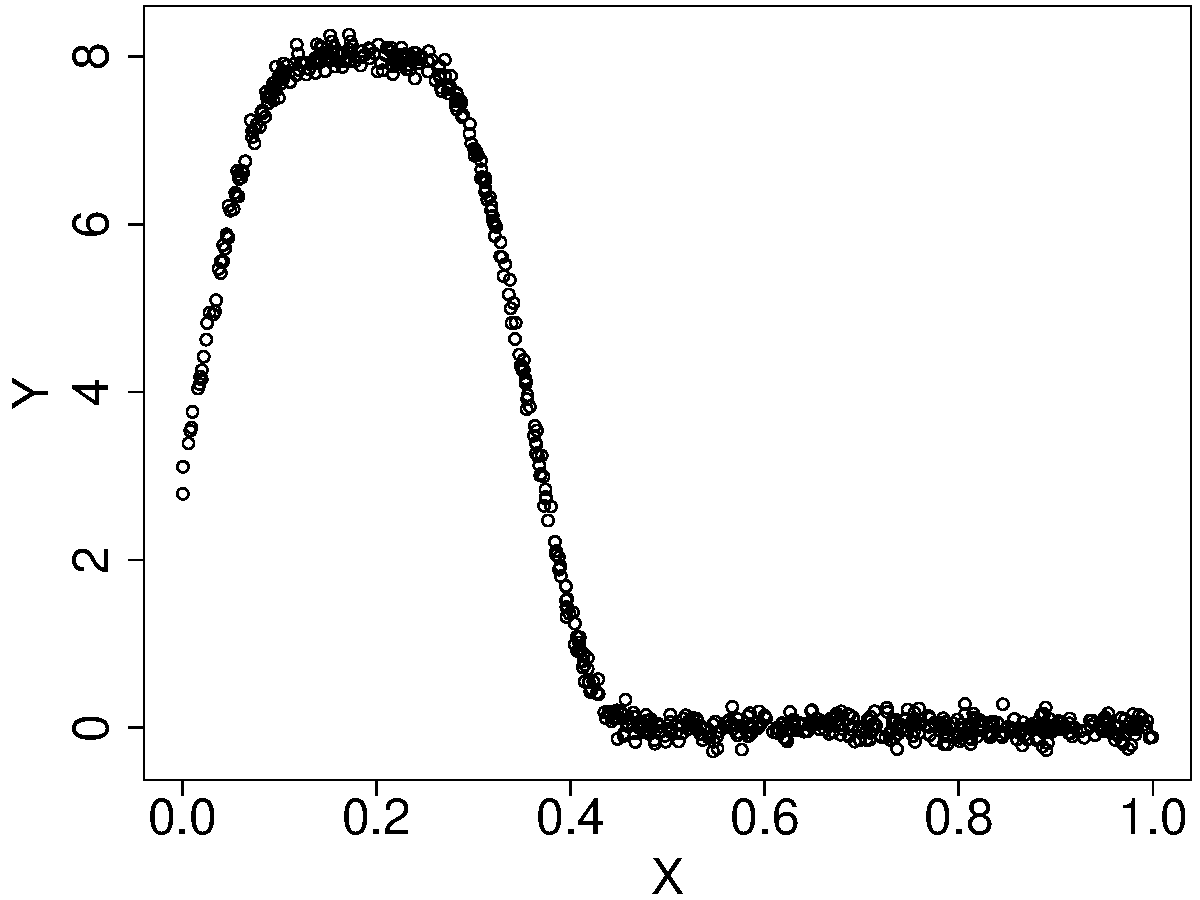
\includegraphics[width=1\linewidth]{Code/Figures/sim7_raw_rep.pdf}
		\caption{Simulated observations from one random run of \eqref{sim7_eq}.}
	\end{subfigure}
	\hfil
	\begin{subfigure}[t]{0.32\linewidth}
		\centering
		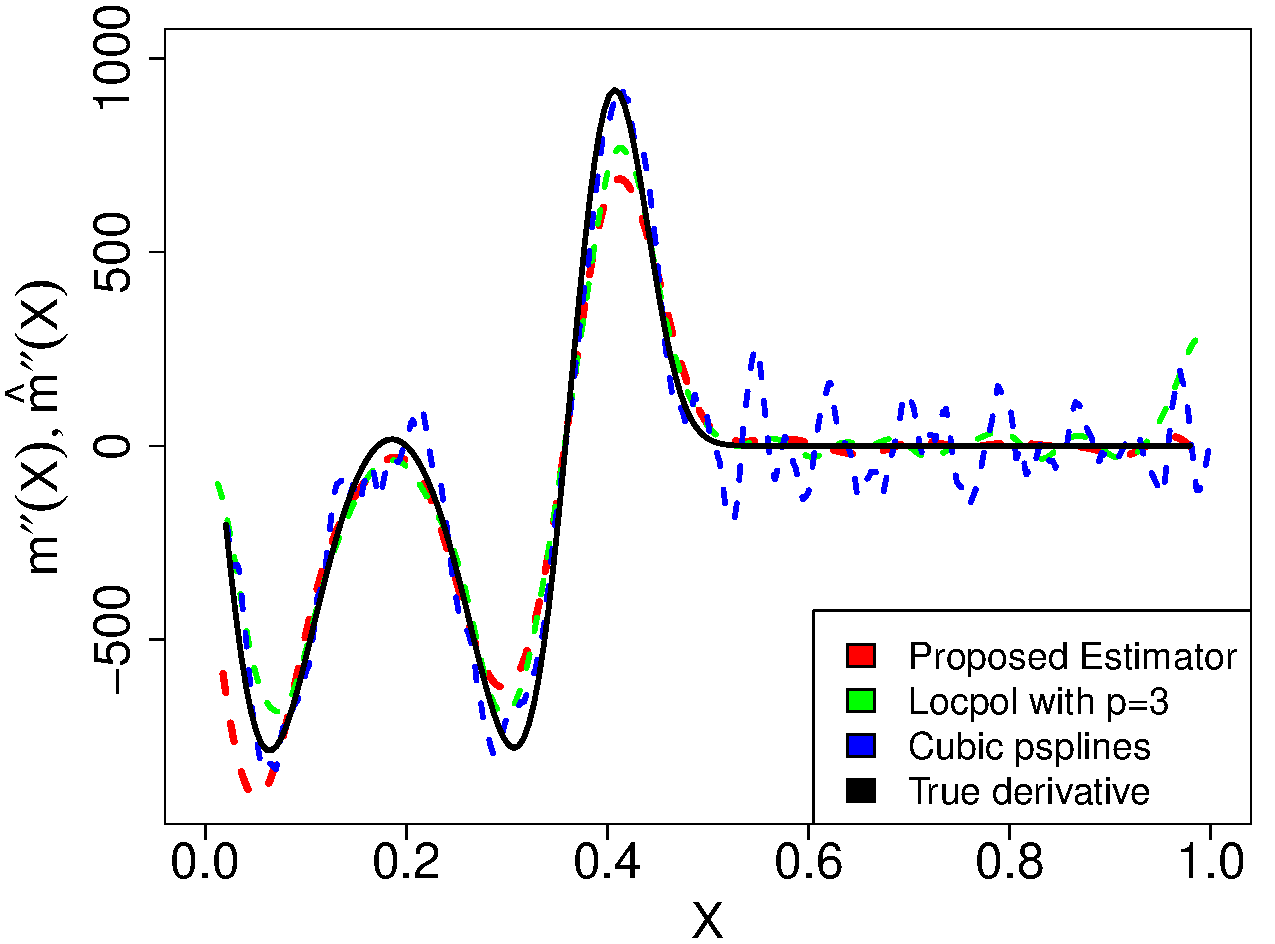
\includegraphics[width=1\linewidth]{Code/Figures/sim7_deriv_com.pdf}
		\caption{Second-order noisy derivatives with chosen $k_1=30, k_2=42$, the smoothed estimates, and the true derivative.}
	\end{subfigure}
	\hfil
	\begin{subfigure}[t]{0.32\linewidth}
		\centering
		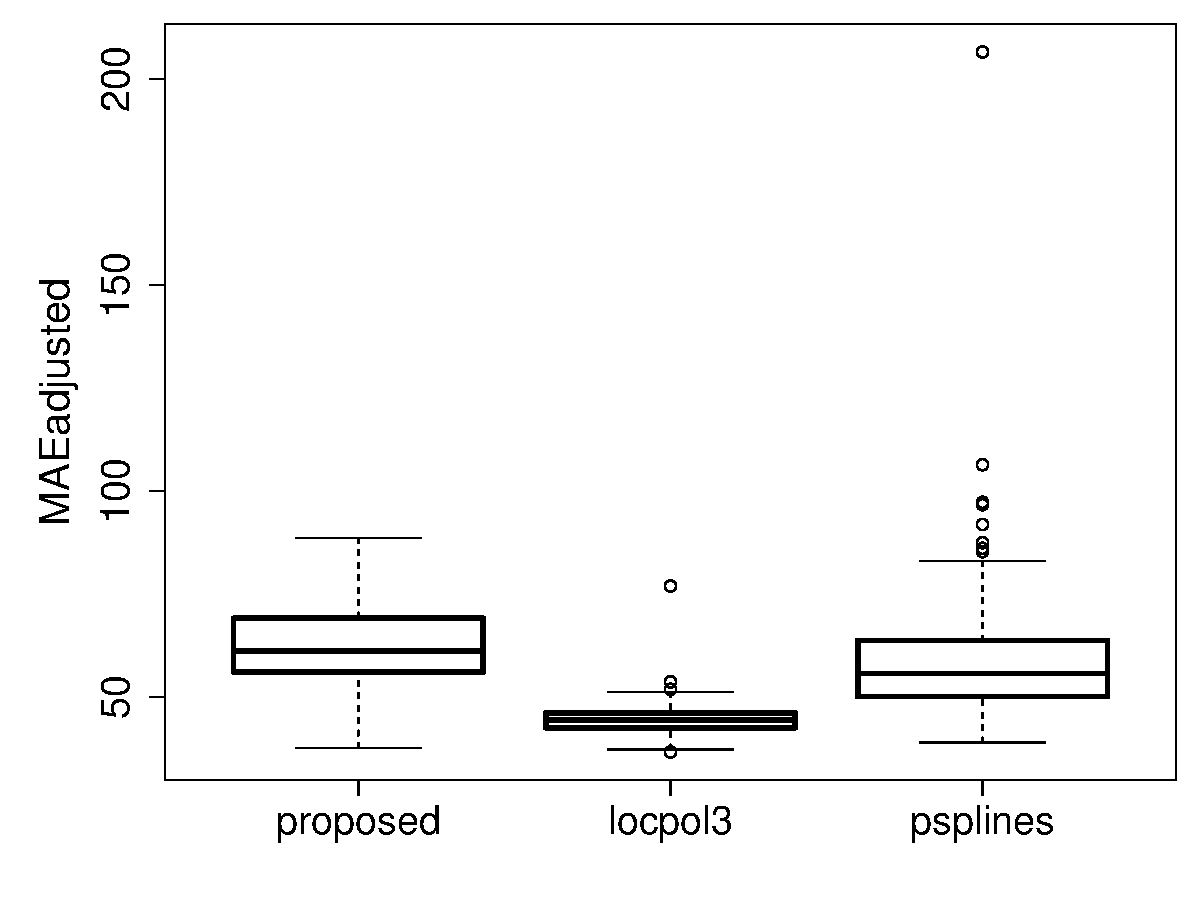
\includegraphics[width=1\linewidth]{Code/Figures/sim7_sec_boxplot.pdf}
		\caption{The proposed smoothed derivative estimates and the derivative of the local polynomial regression with $p=3$.}
	\end{subfigure}
	\caption{{\bf Reproducing Figures 10 and 11 in the paper:} Monte Carlo comparative studies from model \eqref{rand_design} under \eqref{sim7_eq} for the proposed second-order derivative estimator, the local polynomial regression estimator with $p=3$ (``locpol3''), and and penalized smoothing cubic spline estimator (``psplines''). The first row contains figures in the original paper, while the second row presents our reproduced figures.}
	\label{fig:sim7_rep}
\end{figure}

\subsection{Potential Approach for Improving the Estimation Accuracy}
\label{App:poten_improve}

$\bullet$ {\bf Simulation 8:} One reviewer of the paper suggested that it is possible to smooth out the data $\{(X_i,Y_i)\}_{i=1}^n$ by penalized smoothing splines\footnote{The paper claimed that they smoothed out the data via the adaptive splines. However, based on our reproducing work, it is more realistic that the author was smoothing out the data via penalized smoothing cubic splines.} before taking the noisy derivatives. Specifically, we fit a penalized smoothing cubic splines $\hat{m}$ on the data $\{(X_i,Y_i)\}_{i=1}^n$ and compute the difference quotients as:
\begin{equation}
\label{smooth_data}
\frac{\hat{m}(X_{(i)}) - \hat{m}(X_{(i-1)})}{X_{(i)} - X_{(i-1)}} \approx \hat{m}^{(1)}(\xi)
\end{equation}
with $\xi \in \left[X_{(i-1)}, X_{(i)}\right]$. We conduct a Monte Carlo simulation study from model \eqref{rand_design} under \eqref{sim1_eq} and compare our results with the ones in the paper in \autoref{fig:sim8_rep}.

\begin{figure}[!t]
	\captionsetup[subfigure]{justification=centering}
	\begin{subfigure}[t]{0.49\linewidth}
		\centering
		\includegraphics[width=1\linewidth]{Figures_Org/Fig12a.png}
		\caption{Figure 12(a) in the paper.}
	\end{subfigure}
	\hfil
	\begin{subfigure}[t]{0.49\linewidth}
		\centering
		\includegraphics[width=1\linewidth,height=5.2cm]{Figures_Org/Fig12b.png}
		\caption{Figure 12(b) in the paper.}
	\end{subfigure}
	\begin{subfigure}[t]{0.49\linewidth}
		\centering
		\includegraphics[width=1\linewidth]{Code/Figures/sim8_deriv_com.pdf}
		\caption{Comparative results from one random run of model \eqref{sim1_eq}.}
	\end{subfigure}
	\hfil
	\begin{subfigure}[t]{0.49\linewidth}
		\centering
		\includegraphics[width=1\linewidth]{Code/Figures/sim8_deriv_boxplot.pdf}
		\caption{Adjusted mean absolute errors under 100 Monte Carlo repeated experiments.}
	\end{subfigure}
	\caption{{\bf Reproducing Figure 12 in the paper:} Monte Carlo comparative studies from model \eqref{rand_design} under \eqref{sim1_eq} for the proposed first-order derivative estimator with KDE for the distribution of $X$ (``kde''), the proposed first-order derivative estimator under the oracle distribution of $X$ (``uniform''), and the pre-smoothing approach described in \eqref{smooth_data} (``gam''). The first row contains figures in the original paper, while the second row presents our reproduced figures.}
	\label{fig:sim8_rep}
\end{figure}

\subsection{Case Study: Washington State-Level COVID-19 Case Rates}
\label{App:case_study}

Although the discussed paper did not incorporate any real-world application of their proposed methods, we found a potentially interesting real-world application of the derivative estimation on an academic website \url{https://cmu-delphi.github.io/covidcast/modeltoolsR/articles/estimate-deriv.html}. Here, we consider estimating the Washington state-level COVID-19 case rates at the early stage of the pandemic according to the USAFacts data stored in \texttt{R} package \texttt{covidcast} \citep{reinhart2021open}. We restrict the studied dates to the range from ``2020-05-01'' to ``2020-12-15'' at the Washington State, which capture both the initial surge of COVID cases and the first spike during the winter of 2020; see \autoref{fig:case_study}(a). We apply the proposed first-order derivative estimator, local polynomial regression of order $p=2$, and penalized smoothing cubic splines to estimating the case rates within this selected period. The tuning parameter $k$ is selected via Corollary~\ref{cor:k_sel} over the positive integer set $\left\{1,2,...,\floor{\frac{n-1}{2}}\right\}$, where $n$ is the number of dates in this context. The initial bandwidth for the proposed derivative estimator is selected from the set $\{0.001, 0.002,...,0.2\}$. \autoref{fig:case_study} displays the estimated COVID-19 case rates by these three derivative estimation methods, where the proposed derivative estimator with data-driven tuning parameters produce the smoothest estimates. Moreover, the estimated change rates of COVID-19 new cases at the Washington state by the proposed estimator never exceed 71.78\%. Compared with the actual reported cases, however, it is obvious that the increasing rates of COVID-19 cases in November 2020 should be much higher than this number. To some extent, it suggests that the proposed derivative estimators are not quite applicable to the analysis of COVID-19 case rates compared with the other two methods, especially because these rates change rapidly across time and we need more sensible derivative estimators to capture this rapid changing trend for disease control and political decision making.

\begin{figure}[!t]
	\captionsetup[subfigure]{justification=centering}
	\begin{subfigure}[t]{0.49\linewidth}
		\centering
		\includegraphics[width=1\linewidth]{Code/Figures/covid_case_raw.pdf}
		\caption{Reported COVID-19 cases.}
	\end{subfigure}
	\hfil
	\begin{subfigure}[t]{0.49\linewidth}
		\centering
		\includegraphics[width=1\linewidth]{Code/Figures/covid_deriv_com.pdf}
		\caption{Estimated case rates for different methods.}
	\end{subfigure}
	\caption{Reported COVID-19 cases at the Washington state between ``2020-05-01'' and ``2020-12-15'' as well as the estimated case rates by the proposed first-order derivative estimator (``Proposed estimator''), local polynomial regression of order $p=2$ (``Locpol with $p=2$''), and penalized smoothing cubic splines (``Cubic psplines'').}
	\label{fig:case_study}
\end{figure}

\section{Proofs}
\label{App:proofs}

This section supplements the proofs of theorems and theoretical results in the main report. Different from the discussed paper \citep{liu2020smoothed}, I will give a short summary for each proof, fill in more details for the proofs, and rewrite/correct some arguments according to our own understanding. In addition, all the remarks after the proofs are inspired by or extended from the discussed paper.

\subsection{Proof of \autoref{thm:asym_first}}
\label{App:proof_thm1}

\begin{customthm}{1}[Theorem 1 in \citealt{liu2020smoothed}]
Assume that $r$ is twice continuously differentiable on $[0,1]$ under model \eqref{rand_design_unif}. Then, the conditional bias and variance of the first-order noisy derivative estimator \eqref{weight_diff_quo} given $\mathbb{U} = \left(U_{(i-j)},...,U_{(i+j)}\right)$ for $i>j$ and $i+j\leq n$ are 
\begin{align*}
	\left|\mathrm{Bias}\left[\hat{Y}_i^{(1)} \big| \mathbb{U}\right] \right| &\leq \sup_{u\in [0,1]} \left|r^{(2)}(u)\right| \frac{3k(k+1)}{4(n+1)(2k+1)} + o_P\left(\frac{k}{n}\right),\\
	\mathrm{Var}\left[\hat{Y}_i^{(1)} \big| \mathbb{U}\right] &= \frac{3\sigma_e^2 (n+1)^2}{k(k+1)(2k+1)} + o_P\left(\frac{n^2}{k^3}\right)
\end{align*}
uniformly for $k+1\leq i\leq n-k$ when $k\to \infty$ as $n\to \infty$. Further, if we assume that $r$ is $q+1$ times continuously differentiable on $[0,1]$ for $q\geq 1$, then the asymptotic order of the exact conditional bias is given by
\[
\mathrm{Bias}\left[\hat{Y}_i^{(1)} \big| \mathbb{U}\right]=
\begin{cases}
	O_P\left(\frac{k}{n}\right), & q=1,\\
	O_P\left(\max\left\{\frac{k^{\frac{1}{2}}}{n},\, \frac{k^2}{n^2}\right\}\right), & q\geq 2.
\end{cases}
\]
\end{customthm}

\begin{proof}[Proof of \autoref{thm:asym_first}]
{\bf Summary of the Proof:} The proof follows by applying Taylor's theorem over $r$ in model \eqref{rand_design_unif} and using Lemma~\ref{lem:unif_asym} in the calculations of $\left|\mathrm{Bias}\left[\hat{Y}_i^{(1)} \big| \mathbb{U}\right] \right|$ and $\mathrm{Var}\left[\hat{Y}_i^{(1)} \big| \mathbb{U}\right]$.\\

Since $r$ is twice continuously differentiable on $[0,1]$, we have the following Taylor's expansions of $r(U_{(i+j)})$ and $r(U_{(i-j)})$ in the neighborhood of $U_{(i)}$ as:
\begin{align}
\label{r_taylor}
\begin{split}
r(U_{(i+j)}) &= r(U_{(i)}) + \left(U_{(i+j)} -U_{(i)}\right) r^{(1)}(U_{(i)}) + \frac{\left(U_{(i+j)} - U_{(i)}\right)^2}{2} \cdot r^{(2)}(\zeta_{i,i+j}), \\
r(U_{(i-j)}) &= r(U_{(i)}) + \left(U_{(i-j)} -U_{(i)}\right) r^{(1)}(U_{(i)}) + \frac{\left(U_{(i-j)} - U_{(i)}\right)^2}{2} \cdot r^{(2)}(\zeta_{i-j,i}),
\end{split}
\end{align}
where $\zeta_{i,i+j}\in \left[U_{(i)}, U_{(i+j)}\right]$ and $\zeta_{i-j,i} \in \left[U_{(i-j)}, U_{(i)}\right]$. The absolute conditional bias is bounded above by
\begin{align*}
&\left|\mathrm{Bias}\left[\hat{Y}_i^{(1)} \big| \mathbb{U}\right] \right| \\
&= \left|\mathbb{E}\left[\sum_{j=1}^k w_{i,j}\left(\frac{Y_{i+j} - Y_{i-j}}{U_{(i+j)} - U_{(i-j)}}\right) \Big| \mathbb{U} \right] - r^{(1)}(U_{(i)}) \right|\\
&\stackrel{\text{(i)}}{=} \frac{1}{2} \left|\sum_{j=1}^k w_{i,j}\left[\frac{(U_{(i+j)} - U_{(i)})^2 r^{(2)}(\zeta_{i,i+j}) - (U_{(i-j)} - U_{(i)})^2 r^{(2)}(\zeta_{i-j,i})}{U_{(i+j)} - U_{(i-j)}} \right] \right|\\
&\stackrel{\text{(ii)}}{=} \frac{1}{2} \left|\frac{\sum_{j=1}^k (U_{(i+j)} - U_{(i-j)}) \left[(U_{(i+j)} - U_{(i)})^2 \cdot r^{(2)}(\zeta_{i,i+j}) - (U_{(i-j)} - U_{(i)})^2 \cdot r^{(2)}(\zeta_{i-j,i}) \right]}{\sum_{\ell=1}^k \left(U_{(i+\ell)} - U_{(i-\ell)}\right)^2} \right| \\
&\leq \frac{1}{2} \sup_{u\in [0,1]} \left|r^{(2)}(u) \right| \cdot \frac{\sum_{j=1}^k (U_{(i+j)} - U_{(i-j)}) \left[(U_{(i+j)} - U_{(i)})^2 + (U_{(i-j)} - U_{(i)})^2 \right]}{\sum_{\ell=1}^k \left(U_{(i+\ell)} - U_{(i-\ell)}\right)^2}\\
&\stackrel{\text{(iii)}}{=} \frac{1}{2} \sup_{u\in [0,1]} \left|r^{(2)}(u) \right| \cdot \frac{\frac{k^2(k+1)^2}{(n+1)^3}\left[1+ O_P\left(\frac{1}{\sqrt{k}}\right)\right]}{\frac{2k(k+1)(2k+1)}{3(n+1)^2}\left[1+ O_P\left(\frac{1}{\sqrt{k}}\right)\right]}\\
&= \sup_{u\in [0,1]} \left|r^{(2)}(u) \right| \frac{3k(k+1)}{4(n+1)(2k+1)} \left[1+ O_P\left(\frac{1}{\sqrt{k}}\right)\right],
\end{align*}
where (i) follows from \eqref{r_taylor}, (ii) is due to Proposition~\ref{prop:weight_first}, and (iii) is based on Lemma~\ref{lem:unif_asym} and the following calculations as:
\begin{align}
\label{U_sq_bnd}
\begin{split}
\sum_{\ell=1}^k \left(U_{(i+\ell)} - U_{(i-\ell)}\right)^2 &= \sum_{\ell=1}^k \left[\frac{2\ell}{n+1} +O_P\left(\sqrt{\frac{\ell}{n^2}}\right) \right]^2\\
&= \frac{4}{(n+1)^2} \cdot \frac{k(k+1)(2k+1)}{6} + \frac{4}{n+1} \sum_{\ell=1}^k \ell \cdot O_P\left(\sqrt{\frac{\ell}{n^2}}\right) + \sum_{\ell=1}^k O_P\left(\frac{\ell}{n^2}\right)\\
&=\frac{2k(k+1)(2k+1)}{3(n+1)^2}\left[1+ O_P\left(\sqrt{\frac{1}{k}}\right)\right]
\end{split}
\end{align}
and
\begin{align*}
&\sum_{j=1}^k (U_{(i+j)} - U_{(i-j)}) \left[(U_{(i+j)} - U_{(i)})^2 + (U_{(i-j)} - U_{(i)})^2 \right] \\
&= \sum_{j=1}^k \left[\frac{2j}{n+1} +O_P\left(\sqrt{\frac{j}{n^2}}\right) \right] \left\{\left[\frac{j}{n+1} +O_P\left(\sqrt{\frac{j}{n^2}}\right)\right]^2 + \left[\frac{j}{n+1} +O_P\left(\sqrt{\frac{j}{n^2}}\right)\right]^2 \right\} \\
&= \sum_{j=1}^k \frac{4j^3}{(n+1)^3} \left[1+O_P\left(\sqrt{\frac{1}{k}}\right)\right]\\
&= \frac{k^2(k+1)^2}{(n+1)^3} \left[1+O_P\left(\sqrt{\frac{1}{k}}\right)\right].
\end{align*}
Thus, for $k\to \infty$ as $n\to \infty$, 
$$\left|\mathrm{Bias}\left[\hat{Y}_i^{(1)} \big| \mathbb{U}\right] \right| \leq \sup_{u\in [0,1]} \left|r^{(2)}(u)\right| \frac{3k(k+1)}{4(n+1)(2k+1)} + o_P\left(\frac{k}{n}\right).$$
Similarly, by Proposition~\ref{prop:weight_first}, the conditional variance is
\begin{align*}
\mathrm{Var}\left[\hat{Y}_i^{(1)} \big| \mathbb{U}\right] &= \mathrm{Var}\left[\sum_{j=1}^k w_{i,j}\left(\frac{Y_{i+j} - Y_{i-j}}{U_{(i+j)} - U_{(i-j)}}\right) \Big| \mathbb{U} \right] \\
&= 2\sigma_e^2 \cdot \frac{\sum_{j=1}^k \left(U_{(i+j)} - U_{(i-j)}\right)^2}{\left(\sum_{\ell=1}^n (U_{(i+\ell)} - U_{(i-\ell)})^2 \right)^2} \\
&= \frac{2\sigma_e^2}{\sum_{\ell=1}^n (U_{(i+\ell)} - U_{(i-\ell)})^2}\\
&\stackrel{\text{(iv)}}{=} \frac{2\sigma_e^2}{\frac{2k(k+1)(2k+1)}{3(n+1)^2}\left[1+ O_P\left(\sqrt{\frac{1}{k}}\right)\right]}\\
&= \frac{3\sigma_e^2 (n+1)^2}{k(k+1)(2k+1)}\left[1 + o_P(1)\right]
\end{align*}
when $k\to \infty$ as $n\to \infty$, where we leverage our calculation \eqref{U_sq_bnd} in (iv). In addition, the above results hold uniformly for $k+1\leq i \leq n-k$.\\

Now, if $r$ is $q+1$ times continuously differentiable on $[0,1]$ for $q\geq 1$, then applying Taylor's theorem and Lemma~\ref{lem:unif_asym} to $r(U_{(i+j)})$ and $r(U_{(i-j)})$ in a neighborhood of $U_{(i)}$ yields that
\begin{align*}
r(U_{(i+j)}) &= r(U_{(i)}) + \sum_{\ell=1}^{q+1} \frac{r^{(\ell)}(U_{(i)})}{\ell!} \left(U_{(i+j)} - U_{(i)}\right)^{\ell} + O\left(|U_{(i+j)} - U_{(i)}|^{q+2} \right)\\
&= r(U_{(i)}) + \sum_{\ell=1}^{q+1} \frac{r^{(\ell)}(U_{(i)})}{\ell!} \left(U_{(i+j)} - U_{(i)}\right)^{\ell} + O_P\left(\left(\frac{j}{n}\right)^{q+2} \right)
\end{align*}
and 
\begin{align*}
r(U_{(i-j)}) &= r(U_{(i)}) + \sum_{\ell=1}^{q+1} \frac{r^{(\ell)}(U_{(i)})}{\ell!} \left(U_{(i-j)} - U_{(i)}\right)^{\ell} + O\left(|U_{(i-j)} - U_{(i)}|^{q+2} \right)\\
&= r(U_{(i)}) + \sum_{\ell=1}^{q+1} \frac{r^{(\ell)}(U_{(i)})}{\ell!} \left(U_{(i-j)} - U_{(i)}\right)^{\ell} + O_P\left(\left(\frac{j}{n}\right)^{q+2} \right).
\end{align*}
For $q=1$, $r^{(2)}$ exists and is continuous on $[0,1]$, so the conditional bias becomes
\begin{align*}
\mathrm{Bias}\left[\hat{Y}_i^{(1)} \big| \mathbb{U}\right] &= \frac{r^{(1)}(U_{(i)}) \sum_{j=1}^k \left(U_{(i+j)} -U_{(i-j)} \right)^2 + O_P\left(\frac{k^4}{n^3}\right)}{\sum_{\ell=1}^k \left(U_{(i+\ell)} - U_{(i-\ell)}\right)^2} - r^{(1)}(U_{(i)}) \\
&= O_P\left(\frac{k}{n}\right),
\end{align*}
where we can calculate that $\sum_{j=1}^k O_P\left(\left(\frac{j}{n}\right)^{q+2} \right) = O_P\left(\frac{k^{q+3}}{n^{q+2}}\right)$.\\
For $q=2$, $r^{(3)}$ exists on $[0,1]$ and the conditional bias becomes
\begin{align*}
\mathrm{Bias}\left[\hat{Y}_i^{(1)} \big| \mathbb{U}\right] &= \frac{r^{(2)}(U_{(i)}) \sum_{j=1}^k \left(U_{(i+j)} -U_{(i-j)} \right)\left[\left(U_{(i+j)} -U_{(i)}\right)^2 - \left(U_{(i-j)} -U_{(i)}\right)^2\right] + O_P\left(\frac{k^5}{n^4}\right)}{2\sum_{\ell=1}^k \left(U_{(i+\ell)} - U_{(i-\ell)}\right)^2} \\
&=\frac{O_P\left(\frac{k^{\frac{7}{2}}}{n^3}\right) + O_P\left(\frac{k^5}{n^4}\right)}{O_P\left(\frac{k^3}{n^2}\right)}\\
&= O_P\left(\max\left\{\frac{k^{\frac{1}{2}}}{n},\frac{k^2}{n^2}\right\}\right).
\end{align*}
For $q>2$, we can split the conditional bias into even order terms in the Taylor's expansion of $r(U_{(i\pm j)})$ and odd order terms respectively as:
\begin{align*}
\mathrm{Bias}\left[\hat{Y}_i^{(1)} \big| \mathbb{U}\right] &= \frac{\sum_{j=1}^k \left(U_{(i+j)} - U_{(i-j)} \right)\left[\sum\limits_{\ell=3,5,...,2\ceil{q/2}-1} \frac{r^{(\ell)}(U_{(i)})}{\ell!} \left(\left(U_{(i+j)} - U_{(i)} \right)^{\ell} - \left(U_{(i-j)} - U_{(i)} \right)^{\ell} \right) \right]}{\sum_{p=1}^k \left(U_{(i+p)} - U_{(i-p)} \right)^2}\\
&\quad + \frac{\sum_{j=1}^k \left(U_{(i+j)} - U_{(i-j)} \right)\left[\sum\limits_{\ell=2,4,...,2\ceil{q/2}} \frac{r^{(\ell)}(U_{(i)})}{\ell!} \left(\left(U_{(i+j)} - U_{(i)} \right)^{\ell} - \left(U_{(i-j)} - U_{(i)} \right)^{\ell} \right) \right]}{\sum_{p=1}^k \left(U_{(i+p)} - U_{(i-p)} \right)^2} \\
&= \frac{\sum_{j=1}^k \left(U_{(i+j)} - U_{(i-j)} \right)\left[ \frac{r^{(3)}(U_{(i)})}{6} \left(\left(U_{(i+j)} - U_{(i)} \right)^3 - \left(U_{(i-j)} - U_{(i)} \right)^3 \right) \right]}{\sum_{p=1}^k \left(U_{(i+p)} - U_{(i-p)} \right)^2} \left[1+o_P(1)\right]\\
&\quad + \frac{\sum_{j=1}^k \left(U_{(i+j)} - U_{(i-j)} \right)\left[ \frac{r^{(2)}(U_{(i)})}{2} \left(\left(U_{(i+j)} - U_{(i)} \right)^3 - \left(U_{(i-j)} - U_{(i)} \right)^3 \right) \right]}{\sum_{p=1}^k \left(U_{(i+p)} - U_{(i-p)} \right)^2} \left[1+o_P(1)\right]\\
&= \frac{\sum_{j=1}^k \left[\frac{2j}{n+1} + O_P\left(\sqrt{\frac{j}{n^2}}\right)\right] \frac{r^{(3)}(U_{(i)})}{6} \left[\frac{j^3}{(n+1)^3} + O_P\left(\frac{j^{\frac{5}{2}}}{n^3}\right)\right]}{O_P\left(\frac{k^3}{n^2}\right)}\\
&\quad + \frac{\sum_{j=1}^k \left[\frac{2j}{n+1} + O_P\left(\sqrt{\frac{j}{n^2}}\right)\right] \frac{r^{(2)}(U_{(i)})}{2} \cdot O_P\left(\frac{j^{\frac{3}{2}}}{n}\right)}{O_P\left(\frac{k^3}{n^2}\right)}\\
&= O_P\left(\frac{k^2}{n^2}\right) + O_P\left(\frac{k^{\frac{3}{2}}}{n^2}\right) + O_P\left(\frac{k^{\frac{1}{2}}}{n}\right)\\
&= O_P\left(\max\left\{\frac{k^{\frac{1}{2}}}{n},\frac{k^2}{n^2}\right\}\right).
\end{align*}
The proof is thus completed.
\end{proof}

\subsection{Proof of Corollary~\ref{cor:k_sel}}
\label{App:proof_cor2}

\begin{customcor}{2}[Corollary 2 in \citealt{liu2020smoothed}]
Let $\mathcal{B} = \sup_{u\in [0,1]} \left|r^{(2)}(u)\right|$. Under the assumptions of \autoref{thm:asym_first}, the tuning parameter $k$ that minimizes the asymptotic upper bound of the conditional MISE is given by
$$k_{\text{opt}} = \argmin_{k=1,2,...,\floor{\frac{n-1}{2}}} \left[\mathcal{B}^2\frac{9k^2(k+1)^2}{16(n+1)^2(2k+1)^2} + \frac{3\sigma_e^2 (n+1)^2}{k(k+1)(2k+1)} \right].$$
\end{customcor}

\begin{proof}[Proof of Corollary~\ref{cor:k_sel}]
{\bf Summary of the Proof:} The proof follows directly from the definition of the conditional mean integrated squared error (MISE) and the bias-variance decomposition in \autoref{thm:asym_first}.\\

By the bias-variance decomposition in \autoref{thm:asym_first} of the conditional mean squared error, we have that
$$\mathbb{E}\left[\left(\hat{Y}^{(1)}(U) - r^{(1)}(U)\right)^2\big| \mathbb{U}\right] \leq \mathcal{B}^2 \frac{9k^2(k+1)^2}{16(n+1)^2(2k+1)^2} + \frac{3\sigma_e^2 (n+1)^2}{k(k+1)(2k+1)} + o_P\left(\frac{k^2}{n^2} + \frac{n^2}{k^3}\right).$$
Since $U\sim \mathrm{Unif}[0,1]$, the conditional mean integrated squared error (MISE) is given by
\begin{align*}
\mathrm{MISE}\left[\hat{Y}^{(1)}|\mathbb{U}\right] &= \mathbb{E}\left\{\int_0^1 \left[\hat{Y}^{(1)}(U) -r^{(1)}(U)\right]^2 dU \,\Big|\, \mathbb{U}\right\}\\
&= \int_0^1 \mathbb{E}\left[\left(\hat{Y}^{(1)}(U) -r^{(1)}(U)\right)^2 \Big| \mathbb{U} \right] dU\\
&\leq \mathcal{B}^2 \frac{9k^2(k+1)^2}{16(n+1)^2(2k+1)^2} + \frac{3\sigma_e^2 (n+1)^2}{k(k+1)(2k+1)} + o_P\left(\frac{k^2}{n^2} + \frac{n^2}{k^3}\right),
\end{align*}
where $\hat{Y}^{(1)}(U)$ denotes the first-order derivative estimator at design point $U$ and the first two terms comprise the upper bound of the (asymptotic) conditional MISE.
\end{proof}

\begin{Remark}
Selecting the optimal tuning parameter as the minimizer of the asymptotic MISE (\emph{i.e.}, through the bias-variance trade-off; \citealt{wasserman2006all}) is a common approach in Statistics. For instance, all those well-known bandwidth selection methods in kernel density estimation, such as Silverman's rule of thumb (Pages 45 and 47 in \citealt{silverman1986density}), least-square cross validation \citep{hall1983large}, and plug-in method (Section 3.6 in \citealt{wand1994kernel}), are based on the rationale of minimizing the (asymptotic) MISE in different ways. In our context of choosing the number $k$ of weighted difference quotients in \eqref{weight_diff_quo}, we can also solve for $k_{\text{opt}}$ by minimizing the leading terms in Corollary~\ref{cor:k_sel} as:
\begin{align*}
k_{\text{opt}} &= \argmin_{k=1,2,...} \left[\mathcal{B}^2\frac{9k^2(k+1)^2}{16(n+1)^2(2k+1)^2} + \frac{3\sigma_e^2 (n+1)^2}{k(k+1)(2k+1)} \right] \\
&\approx \argmin_{k=1,2,...} \left[\mathcal{B}^2\frac{9k^2}{64n^2} + \frac{3\sigma_e^2 n^2}{2k^3} \right]\\
&= \floor{2 \sigma_e^{\frac{2}{5}} \mathcal{B}^{-\frac{2}{5}} n^{\frac{4}{5}}},
\end{align*}
where the unknown quantities $\mathcal{B}$ and $\sigma_e^2$ can be estimated according to our suggestions in Section~\ref{Sec:first_asymp}.
\end{Remark}

\subsection{Proof of \autoref{thm:loc_poly_first}}
\label{App:proof_thm3}

\begin{customthm}{3}[Theorem 2 in \citealt{liu2020smoothed}]
Assume that $r(\cdot)$ under model \eqref{rand_design_unif} is $(p+2)$ times continuously differentiable in a neighborhood of $u_0$. Under Assumptions~\ref{assump:kernel} and \ref{assump:cor_func}, the conditional bias and variance of \eqref{loc_poly_first} with $u_0\in [0,1]$ for $p$ odd are
\begin{align*}
	\mathrm{Bias}\left[\hat{r}^{(1)}(u_0) | \tilde{\mathbb{U}}\right] &\leq\left[\bm{\epsilon}_1^T \bm{S}^{-1}c_p\cdot \frac{r^{(p+2)}(u_0)}{(p+1)!} \cdot h^{p+1} + \left|\bm{\epsilon}_1^T \bm{S}^{-1} \right|\tilde{c}_p \cdot \frac{3k(k+1) \mathcal{B}}{4(n+1)(2k+1)}\right] \left[1+o_P(1)\right]\\
	&= \left[\left(\int t^{p+1} K_0^{\star}(t) dt\right) \frac{r^{(p+2)}(u_0)}{(p+1)!} \cdot h^{p+1} + \left|\bm{\epsilon}_1^T \bm{S}^{-1}\right| \tilde{c}_p \cdot\frac{3k(k+1) \mathcal{B}}{4(n+1)(2k+1)}\right] \left[1+o_P(1)\right],\\
	\mathrm{Var}\left[\hat{r}^{(1)}(u_0) | \tilde{\mathbb{U}}\right] &= \frac{3\sigma_e^2 (n+1)^2 (1+\rho_c)}{k(k+1)(2k+1) (n-2k) h} \cdot \bm{\epsilon}_1^T \bm{S}^{-1} \bm{S}^* \bm{S}^{-1} \bm{\epsilon}_1 \left[1+o_P(1)\right]\\
	&= \left(\int K_0^{\star}(t)^2 dt \right) \frac{3\sigma_e^2 (n+1)^2 (1+\rho_c)}{k(k+1)(2k+1) (n-2k) h} \left[1+o_P(1)\right]
\end{align*}
as $h\to 0, nh\to \infty, k\to \infty$ with $n\to \infty$, where $\tilde{\mathbb{U}}=\left(U_{(1)},...,U_{(n)}\right)$, $\mathcal{B}=\sup_{u\in [0,1]}\left|r^{(2)}(u) \right|$, $\bm{S}=\left(\mu_{i+j-2}\right)_{1\leq i,j\leq p+1}$ with $\mu_j=\int u^j K(u) du$, $\bm{S}^*=\left(\nu_{i+j-2}\right)_{1\leq i,j\leq p+1}$ with $\nu_j = \int u^j K(u)^2 du$, $c_p=\left(\mu_{p+1},...,\mu_{2p+1} \right)^T$, $\tilde{c}_p=\left(\tilde{\mu}_0,...,\tilde{\mu}_{p} \right)^T$ with $\tilde{\mu}_j=\int |u|^j K(u) du$, $\bm{\epsilon}_1=(1,0,...,0)^T \in \mathbb{R}^{p+1}$, $\left|\bm{\epsilon}_1^T\bm{S}^{-1}\right|$ means elementwise absolute values of $\bm{\epsilon}_1^T\bm{S}^{-1}$, and the equivalent kernel $K_0^{\star}(t) = \bm{\epsilon}_1^T \bm{S}^{-1} \left(1,t,...,t^p\right)^T K(t)$.
\end{customthm}

\begin{proof}[Proof of \autoref{thm:loc_poly_first}]
{\bf Summary of the Proof:} The proof follows from the arguments of Theorem 3.1 in \cite{fan1996local} (see its Section 3.7) and the results of Theorem 1 in \cite{de2018local}. In particular, we derive the asymptotic expression for each entry of the matrix $\bm{S}_{n-2k}\equiv \bm{S}_{u_0}$ in \eqref{loc_poly_first} and utilize the identity
$$(A+hB)^{-1} = A^{-1} - hA^{-1} B A^{-1} + O(h^2)$$
to handle the asymptotic expression of $\bm{S}_{n-2k}^{-1}$. Notice that there is an incorrect inequality (Eq.(31) on Page 34 of the discussed paper) in the original proof of this theorem in \cite{liu2020smoothed}. I fix this minor mistake in the following argument by slightly changing the statement of \autoref{thm:loc_poly_first} here.\\

$\bullet$ {\bf Conditional variance:} Recall from \autoref{thm:asym_first} that when $k\to \infty$ as $n\to\infty$, 
$$\mathrm{Var}\left[\hat{Y}_i^{(1)} \big| \tilde{\mathbb{U}}\right] = \frac{3\sigma_e^2 (n+1)^2}{k(k+1)(2k+1)}\left[1+ o_P(1)\right].$$
By Theorem 1 in \cite{de2018local} and the definition of $\hat{r}^{(1)}(u_0)$ in \eqref{loc_poly_first}, we have that
\begin{align*}
\mathrm{Var}\left[\hat{r}^{(1)}(u_0) \big| \tilde{\mathbb{U}}\right] &= \bm{\epsilon}_1^T \bm{S}_{n-2k}^{-1} \left(\bm{U}_{u_0}^T \bm{W}_{u_0} \cdot \mathrm{Var}\left[\hat{\bm{Y}}^{(1)} \big| \tilde{\mathbb{U}}\right] \cdot \bm{W}_{u_0} \bm{U}_{u_0}\right) \bm{S}_{n-2k}^{-1} \bm{\epsilon}_1\\
&= \frac{3\sigma_e^2 (n+1)^2}{k(k+1)(2k+1)} \cdot \frac{1 + f(u_0)\rho_c}{h(n-2k) f(u_0)}\cdot \bm{\epsilon}_1^T \bm{S}^{-1} \bm{S}^* \bm{S}^{-1} \bm{\epsilon}_1\left[1+ o_P(1)\right]\\
&= \frac{3\sigma_e^2 (n+1)^2}{k(k+1)(2k+1)} \cdot \frac{1 + \rho_c}{h(n-2k)}\cdot \bm{\epsilon}_1^T \bm{S}^{-1} \bm{S}^* \bm{S}^{-1} \bm{\epsilon}_1\left[1+ o_P(1)\right]
\end{align*}
under Assumptions~\ref{assump:kernel} and \ref{assump:cor_func}, where  $\bm{S}^*=\left(\nu_{i+j-2}\right)_{1\leq i,j\leq p+1}$ with $\nu_j = \int u^j K(u)^2 du$ and $f(u_0)=1$ for any $u_0\in [0,1]$. By the definition of the equivalent kernel (see also Section 3.2.2 in \citealt{fan1996local}), one can also write
\begin{align*}
\mathrm{Var}\left[\hat{r}^{(1)}(u_0) \big| \tilde{\mathbb{U}}\right] &= \frac{3\sigma_e^2 (n+1)^2}{k(k+1)(2k+1)} \cdot \frac{1 + \rho_c}{h(n-2k)}\cdot \bm{\epsilon}_1^T \bm{S}^{-1} \bm{S}^* \bm{S}^{-1} \bm{\epsilon}_1\left[1+ o_P(1)\right] \\
&= \left(\int K_0^{\star}(t)^2 dt \right) \frac{3\sigma_e^2 (n+1)^2 (1+\rho_c)}{k(k+1)(2k+1) (n-2k) h} \left[1+o_P(1)\right],
\end{align*}
given that $\int K_0^{\star}(t)^2 dt = \bm{\epsilon}_1^T \bm{S}^{-1}\bm{S}^* \bm{S}^{-1} \bm{\epsilon}_1$.\\

$\bullet$ {\bf Conditional bias:} Notice from \eqref{loc_poly_first} that
\begin{align}
\label{cond_bias_loc_poly}
\begin{split}
\mathrm{Bias}\left[\hat{r}^{(1)}(u_0) \big| \tilde{\mathbb{U}}\right] &= \mathbb{E}\left[\hat{r}^{(1)}(u_0) \big| \tilde{\mathbb{U}}\right] - r^{(1)}(u_0)\\
&= \bm{\epsilon}_1^T \bm{S}_{n-2k}^{-1} \bm{U}_{u_0}^T \bm{W}_{u_0} \cdot \mathbb{E}\left[\hat{\bm{Y}}^{(1)} \big| \tilde{\mathbb{U}}\right] - r^{(1)}(u_0)\\
&= \bm{\epsilon}_1^T \bm{S}_{n-2k}^{-1} \bm{U}_{u_0}^T \bm{W}_{u_0} \left(\begin{bmatrix}
r^{(1)}(U_{(k+1)})\\
\vdots\\
r^{(1)}(U_{(n-k)})
\end{bmatrix} + \begin{bmatrix}
\mathrm{Bias}\left[\hat{Y}_{k+1}^{(1)} \big|\tilde{\mathbb{U}}\right]\\
\vdots\\
\mathrm{Bias}\left[\hat{Y}_{n-k}^{(1)} \big|\tilde{\mathbb{U}}\right]\\
\end{bmatrix}\right) -r^{(1)}(u_0)\\
&= \underbrace{\bm{\epsilon}_1^T \bm{S}_{n-2k}^{-1} \bm{U}_{u_0}^T \bm{W}_{u_0} \begin{bmatrix}
	r^{(1)}(U_{(k+1)})\\
	\vdots\\
	r^{(1)}(U_{(n-k)})
\end{bmatrix} -r^{(1)}(u_0)}_{\text{Term I}} + \underbrace{\bm{\epsilon}_1^T \bm{S}_{n-2k}^{-1} \bm{U}_{u_0}^T \bm{W}_{u_0}\begin{bmatrix}
\mathrm{Bias}\left[\hat{Y}_{k+1}^{(1)} \big|\tilde{\mathbb{U}}\right]\\
\vdots\\
\mathrm{Bias}\left[\hat{Y}_{n-k}^{(1)} \big|\tilde{\mathbb{U}}\right]\\
\end{bmatrix}}_{\text{Term II}}.
\end{split}
\end{align}
By direct calculations, 
\begin{align*}
\bm{S}_{n-2k} = \bm{U}_{u_0}^T \bm{W}_{u_0}\bm{U}_{u_0} &= 
\begin{bmatrix}
S_{n-2k,0} & S_{n-2k,1} & \cdots & S_{n-2k,p}\\
S_{n-2k,1} & S_{n-2k,2} & \cdots & S_{n-2k,p+1}\\
\vdots & \vdots & \ddots & \vdots\\
S_{n-2k,p} & S_{n-2k,p+1} & \cdots & S_{n-2k,2p}
\end{bmatrix},
\end{align*}
where 
$$S_{n-2k,\ell} = \sum_{m=k+1}^{n-k} \left(U_{(m)} -u_0\right)^{\ell} K\left(\frac{U_{(m)} -u_0}{h} \right) = \mathbb{E}\left[S_{n-2k,\ell}\right] + O_P\left(\sqrt{\mathrm{Var}\left[S_{n-2k,\ell}\right]}\right)$$ 
for $\ell=0,1,...,2p$. More importantly, $U_{(k+1)},...,U_{(n-k)}$ can be regarded as an i.i.d. sample when we sum over $k+1,...,n-k$ as in $S_{n-2k,\ell}$. Thus, when $h\to 0$ and $nh\to \infty$ as $n\to \infty$, we have that
\begin{align*}
\mathbb{E}\left[S_{n-2k,\ell}\right] &= (n-2k) \cdot \mathbb{E}\left[(U-u_0)^{\ell} K\left(\frac{U-u_0}{h}\right) \right]\\
&= (n-2k) \int K\left(\frac{u-u_0}{h}\right) (u-u_0)^{\ell} f(u) du\\
&= (n-2k) h^{\ell+1} \int K(x) x^{\ell} f(u_0+hx) dx\\
&= (n-2k) h^{\ell+1} f(u_0)\left[\int x^{\ell} K(x) dx + O(h)\right]\\
&= (n-2k) h^{\ell+1} f(u_0)\mu^{\ell} \left[1+ O(h)\right]
\end{align*}
and 
\begin{align*}
O_P\left(\sqrt{\mathrm{Var}\left[S_{n-2k,\ell}\right]}\right) &= O_P\left(\sqrt{(n-2k) \cdot \mathbb{E}\left[(U-u_0)^{2\ell} \cdot K\left(\frac{U-u_0}{h}\right)^2 \right]} \right)\\
&= O_P\left(\sqrt{(n-2k) \int (u-u_0)^{2\ell} K\left(\frac{u-u_0}{h}\right)^2 f(u) du} \right)\\
&= O_P\left(\sqrt{(n-2k) h^{2\ell +1} f(u_0) \int x^{2\ell} K^2(x) dx} \right)\\
&= O_P\left(\sqrt{(n-2k) h^{2\ell+1}} \right).
\end{align*}
These results imply that, for $h\to 0$, $nh\to \infty$, and $k\to \infty$ with $\frac{k}{n} \to 0$ as $n\to \infty$, 
\begin{align*}
S_{n-2k,\ell} &= (n-2k) h^{\ell +1} f(u_0) \mu_{\ell} \left[1+ O(h) + O_P\left(\sqrt{\frac{1}{(n-2k)h}}\right)\right]
\end{align*}
so that 
\begin{align*}
\bm{S}_{n-2k} &= 
\begin{bmatrix}
	S_{n-2k,0} & S_{n-2k,1} & \cdots & S_{n-2k,p}\\
	S_{n-2k,1} & S_{n-2k,2} & \cdots & S_{n-2k,p+1}\\
	\vdots & \vdots & \ddots & \vdots\\
	S_{n-2k,p} & S_{n-2k,p+1} & \cdots & S_{n-2k,2p}
\end{bmatrix} = (n-2k)h f(u_0) \bm{H}\bm{S}\bm{H}\left[1 + o_P(1)\right],
\end{align*}
where $\bm{H} = \Diag\left(1,h,...,h^p\right)$ and $\bm{S}=\left(\mu_{i+j-2}\right)_{1\leq i,j\leq p+1}$ with $\mu_j=\int u^j K(u) du$.

\emph{Term I in \eqref{cond_bias_loc_poly}:} When $p$ is odd, we can directly leverage the results of Theorem 3.1 in \cite{fan1996local} to obtain that
\begin{align*}
\text{Term I} &= \bm{\epsilon}_1^T \bm{S}_{n-2k}^{-1} \bm{U}_{u_0}^T \bm{W}_{u_0} \begin{bmatrix}
	r^{(1)}(U_{(k+1)})\\
	\vdots\\
	r^{(1)}(U_{(n-k)})
\end{bmatrix} -r^{(1)}(u_0) \\
&= \bm{\epsilon}_1^T \bm{S}_{n-2k}^{-1} \bm{U}_{u_0}^T \bm{W}_{u_0} \left(\begin{bmatrix}
	r^{(1)}(U_{(k+1)})\\
	\vdots\\
	r^{(1)}(U_{(n-k)})
\end{bmatrix} - \bm{U}_{u_0} \bm{\beta}_{u_0}\right)\\
&= \bm{\epsilon}_1^T \bm{S}_{n-2k}^{-1} \bm{U}_{u_0}^T \bm{W}_{u_0} \begin{bmatrix}
r^{(1)}(U_{(k+1)}) - \sum_{j=0}^p \left(U_{(k+1)} - u_0\right)^j \cdot \frac{r^{(j+1)}(u_0)}{j!}\\
\vdots\\
r^{(1)}(U_{(n-k)}) - \sum_{j=0}^p \left(U_{(n-k)} - u_0\right)^j \cdot \frac{r^{(j+1)}(u_0)}{j!}\\
\end{bmatrix}\\
&\stackrel{\text{(i)}}{=} \bm{\epsilon}_1^T \bm{S}_{n-2k}^{-1} \bm{U}_{u_0}^T \bm{W}_{u_0} 
\begin{bmatrix}
\frac{r^{(p+2)}(u_0)}{(p+1)!} (U_{(k+1)}- u_0)^{p+1} + o\left((U_{(k+1)} -u_0)^{p+1}\right)\\
\vdots\\
\frac{r^{(p+2)}(u_0)}{(p+1)!} (U_{(n-k)}- u_0)^{p+1} + o\left((U_{(n-k)} -u_0)^{p+1}\right)\\
\end{bmatrix}\\
&\stackrel{\text{(ii)}}{=} \bm{\epsilon}_1^T \big\{(n-2k)h f(u_0) \bm{H}\bm{S}\bm{H}\left[1 + O(h)\right]\big\}^{-1} \cdot\frac{r^{(p+2)}(u_0)}{(p+1)!} \cdot (n-2k)h^{p+2}\bm{H} c_p \left[1+O(h)\right]\\
&\stackrel{\text{(iii)}}{=} \bm{\epsilon}_1^T \bm{S}^{-1}c_p \cdot \frac{r^{(p+2)}(u_0)}{(p+1)!} \cdot h^{p+1} + o_P\left(h^{p+1}\right),
\end{align*}
where $\bm{\beta}_{u_0}=\left(r^{(1)}(u_0),...,\frac{r^{(p+1)}(u_0)}{p!}  \right)^T \in \mathbb{R}^{p+1}$ and $c_p=\left(\mu_{p+1},...,\mu_{2p+1} \right)^T\in \mathbb{R}^{p+1}$. Here, we use the Taylor's expansion of $r^{(1)}$ around $u_0$ in equality (i), apply the asymptotic expressions for $\bm{S}_{n-2k}$ and $\bm{U}_{u_0}^T \bm{W}_{u_0}$ in equality (ii), and utilize the identity $(A+hB)^{-1} = A^{-1} - hA^{-1} B A^{-1} + O(h^2)$ in equality (iii).

\emph{Term II:} According to \autoref{thm:asym_first}, we know that, for $k\to \infty$ as $n\to \infty$,
\begin{align*}
\text{Term II} &= \bm{\epsilon}_1^T \bm{S}_{n-2k}^{-1} \bm{U}_{u_0}^T \bm{W}_{u_0}\begin{bmatrix}
	\mathrm{Bias}\left[\hat{Y}_{k+1}^{(1)} \big|\tilde{\mathbb{U}}\right]\\
	\vdots\\
	\mathrm{Bias}\left[\hat{Y}_{n-k}^{(1)} \big|\tilde{\mathbb{U}}\right]\\
\end{bmatrix}\\
&= \bm{\epsilon}_1^T \bm{S}_{n-2k}^{-1} 
\begin{bmatrix}
\sum_{m=k+1}^{n-k} \text{Bias}\left[\hat{Y}_m^{(1)} \big| \tilde{\mathbb{U}}\right] K\left(\frac{U_{(m)}-u_0}{h}\right)\\
\sum_{m=k+1}^{n-k} \text{Bias}\left[\hat{Y}_m^{(1)} \big| \tilde{\mathbb{U}}\right] \left(U_{(m)} -u_0\right) K\left(\frac{U_{(m)}-u_0}{h}\right)\\
\vdots\\
\sum_{m=k+1}^{n-k} \text{Bias}\left[\hat{Y}_m^{(1)} \big| \tilde{\mathbb{U}}\right] \left(U_{(m)} -u_0\right)^p K\left(\frac{U_{(m)}-u_0}{h}\right)
\end{bmatrix}\\
&\leq \left|\bm{\epsilon}_1^T  \big\{(n-2k)h f(u_0) \bm{H}\bm{S}\bm{H}\left[1 + O(h)\right]\big\}^{-1} \right|  (n-2k)h\bm{H} \tilde{c}_p \left[1+O(h)\right] \cdot \frac{3k(k+1)\mathcal{B}}{4(n+1)(2k+1)} \\
&= \left|\bm{\epsilon}_1^T \bm{S}^{-1}\right| \tilde{c}_p\cdot \frac{3k(k+1)\mathcal{B}}{4(n+1)(2k+1)}\cdot\left[1+o_P(1)\right]
\end{align*}
where $\mathcal{B}= \sup_{u\in [0,1]}\left|r^{(2)}(u) \right|$ and $\tilde{c}_p=\left(\tilde{\mu}_0,...,\tilde{\mu}_{p} \right)^T$ with $\tilde{\mu}_j=\int |u|^j K(u) du$.

Combining \emph{Term I} and \emph{Term II} with \eqref{cond_bias_loc_poly} yields that
\begin{align*}
\mathrm{Bias}\left[\hat{r}^{(1)}(u_0) \big| \tilde{\mathbb{U}}\right] &= \bm{\epsilon}_1^T \bm{S}_{n-2k}^{-1} \bm{U}_{u_0}^T \bm{W}_{u_0} \begin{bmatrix}
		r^{(1)}(U_{(k+1)})\\
		\vdots\\
		r^{(1)}(U_{(n-k)})
	\end{bmatrix} -r^{(1)}(u_0) + \bm{\epsilon}_1^T \bm{S}_{n-2k}^{-1} \bm{U}_{u_0}^T \bm{W}_{u_0}\begin{bmatrix}
		\mathrm{Bias}\left[\hat{Y}_{k+1}^{(1)} \big|\tilde{\mathbb{U}}\right]\\
		\vdots\\
		\mathrm{Bias}\left[\hat{Y}_{n-k}^{(1)} \big|\tilde{\mathbb{U}}\right]\\
\end{bmatrix}\\
&\leq \left[\bm{\epsilon}_1^T \bm{S}^{-1}c_p\cdot \frac{r^{(p+2)}(u_0)}{(p+1)!} \cdot h^{p+1} + \left|\bm{\epsilon}_1^T \bm{S}^{-1} \right| \tilde{c}_p \cdot \frac{3k(k+1) \mathcal{B}}{4(n+1)(2k+1)}\right] \left[1+o_P(1)\right]\\
&= \left[\left(\int t^{p+1} K_0^{\star}(t) dt\right) \frac{r^{(p+2)}(u_0)}{(p+1)!} \cdot h^{p+1} + \left|\bm{\epsilon}_1^T \bm{S}^{-1}\right| \tilde{c}_p \cdot\frac{3k(k+1) \mathcal{B}}{4(n+1)(2k+1)}\right] \left[1+o_P(1)\right],
\end{align*}
where $\int t^{p+1} K_0^{\star}(t) dt= \bm{\epsilon}_1^T \bm{S}^{-1} c_p$. The results follow.
\end{proof}

\begin{Remark}
\label{remark:MISE_loc_poly}
Under the assumptions of \autoref{thm:loc_poly_first}, the conditional mean integrated squared error (MISE) of the local polynomial regression estimator \eqref{loc_poly_first} is upper bounded by
\begin{align*}
&\mathrm{MISE}\left[\hat{r}^{(1)} \big|\tilde{\mathbb{U}}\right] \\
&= \mathbb{E}\left\{\int_0^1 \left[\hat{r}^{(1)}(u_0) -r^{(1)}(u_0)\right]^2 du_0 \,\Big|\, \tilde{\mathbb{U}}\right\}\\
&= \int_0^1 \mathbb{E}\left[\left(\hat{r}^{(1)}(u_0) -r^{(1)}(u_0)\right)^2 \Big| \tilde{\mathbb{U}} \right] du_0\\
&\leq \left[\left|\int t^{p+1} K_0^{\star}(t) dt\right| \frac{\sup_{u\in [0,1]}\left|r^{(p+2)}(u)\right|}{(p+1)!} \cdot h^{p+1} + \left|\bm{\epsilon}_1^T \bm{S}^{-1} \right| \tilde{c}_p\cdot \frac{3k(k+1) \mathcal{B}}{4(n+1)(2k+1)}\right]^2 \left[1+o_P(1)\right] \\
&\quad + \left(\int K_0^{\star}(t)^2 dt \right) \frac{3\sigma_e^2 (n+1)^2 (1+\rho_c)}{k(k+1)(2k+1) (n-2k) h} \left[1+o_P(1)\right] \\
&= O_P\left(h^{2p+2}\right) + O_P\left(\frac{kh^{p+1}}{n}\right) + O_P\left(\frac{k^2}{n^2}\right) + O_P\left(\frac{n}{k^3h}\right),
\end{align*}
given that $k$ is always of smaller order than $O(n)$. By taking the partial derivatives with respect to $h$ and $k$ and setting them to 0, we obtain a system of equations
\[
\begin{cases}
h^{2p+1} + \frac{kh^p}{n} - \frac{n}{k^3h^2} \asymp 0,\\
\frac{h^{p+1}}{n} + \frac{k}{n^2} - \frac{n}{k^4 h} \asymp 0,
\end{cases}
\]
where we introduce the asymptotic equivalence symbol ``$\asymp$'' to get rid of all the constant factors. Solving this system of equations gives us that $k=O\left(n^{\frac{3p+4}{5p+6}}\right)$ and $h=O\left(n^{-\frac{2}{5p+6}}\right)$, which leading to an optimal rate of convergence for the upper bound of $\mathrm{MISE}\left[\hat{r}^{(1)} \big|\tilde{\mathbb{U}}\right]$ as $O_P\left(n^{-\frac{4p+4}{5p+6}}\right)$.
\end{Remark}

\subsection{Proof of \autoref{thm:asym_second}}
\label{App:proof_thm5}

\begin{customthm}{5}[Theorem 3 in \citealt{liu2020smoothed}]
Assume that $r$ is three times continuously differentiable on $[0,1]$ under model \eqref{rand_design_unif}. Then, under the weight $w_{ij,2}=\frac{(2j+k_1)^2}{\sum_{j=1}^{k_2} (2j+k_1)^2}$, the conditional bias and variance of the second-order noisy derivative estimator \eqref{weighted_DQ_second} given $\tilde{\mathbb{U}}=\left(U_{(1)},..., U_{(n)}\right)$ are bounded by
\begin{align*}
	\left|\mathrm{Bias}\left[\hat{Y}_i^{(2)} \big| \tilde{\mathbb{U}}\right] \right| &\leq \frac{\sup_{u\in [0,1]}\left|r^{(3)}(u)\right|}{n+1}  \left(\frac{2\sum_{j=1}^{k_2} j^3 + 3k_1 \sum_{j=1}^{k_2} j^2 + \frac{5}{3} k_1^2 \sum_{j=1}^{k_2}j + \frac{1}{3} k_1^3k_2}{4 \sum_{j=1}^{k_2}j^2 + k_1^2k_2 + 4k_1\sum_{j=1}^{k_2} j} \right)\left[1+o_P(1)\right],\\
	\mathrm{Var}\left[\hat{Y}_i^{(2)} \big| \tilde{\mathbb{U}}\right] &\leq \frac{4(n+1)^4 \sigma_e^2}{k_1^2 \sum_{j=1}^{k_2} (2j+k_1)^2} \cdot \left[1+o_P(1)\right]
\end{align*}
uniformly for $k_1+k_2+1 \leq i\leq n-k_1-k_2$ when $k_1,k_2\to \infty$ as $n\to\infty$.
\end{customthm}

\begin{proof}[Proof of \autoref{thm:asym_second}]
{\bf Summary of the Proof:} The proof is similar to our arguments in Appendix~\ref{App:proof_thm1} for the proof of \autoref{thm:asym_first}. In particular, we apply Taylor's theorem to the function $r$ and utilize Lemma~\ref{lem:unif_asym} to handle the asymptotic terms in $\left|\mathrm{Bias}\left[\hat{Y}_i^{(2)} \big| \tilde{\mathbb{U}}\right] \right|$ and $\mathrm{Var}\left[\hat{Y}_i^{(2)} \big| \tilde{\mathbb{U}}\right]$.\\

Since $r$ is three times continuously differentiable on $[0,1]$, we have the following Taylor's expansions of $r(U_{(i+j+k_1)})$ and $r(U_{(i-j-k_1)})$ in the neighborhoods of $U_{(i+j)}$ and $U_{(i-j)}$ respectively as:
\begin{align}
\label{taylor1}
\begin{split}
r(U_{(i+j+k_1)}) &= \sum_{q=0}^2 \frac{\left(U_{(i+j+k_1)} - U_{(i+j)}\right)^q}{q!} \cdot r^{(q)}(U_{(i+j)}) + \frac{\left(U_{(i+j+k_1)} - U_{(i+j)}\right)^3}{6} \cdot r^{(3)}(\zeta_{i+j,i+j+k_1}),\\
r(U_{(i-j-k_1)}) &= \sum_{q=0}^2 \frac{\left(U_{(i-j-k_1)} - U_{(i-j)}\right)^q}{q!} \cdot r^{(q)}(U_{(i-j)}) + \frac{\left(U_{(i-j-k_1)} - U_{(i-j)}\right)^3}{6} \cdot r^{(3)}(\zeta_{i-j-k_1,i-j}),
\end{split}
\end{align}
where $\zeta_{i+j,i+j+k_1} \in \left[U_{(i+j)}, U_{(i+j+k_1)}\right]$ and $\zeta_{i-j-k_1,i-j} \in \left[U_{(i-j-k_1)}, U_{(i-j)}\right]$. In addition, the following Taylor's expansions of $r^{(1)}(U_{(i+j)})$ and $r^{(1)}(U_{(i-j)})$ are also valid in a neighborhood of $U_{(i)}$ as:
\begin{align}
\label{taylor2}
\begin{split}
r^{(1)}(U_{(i+j)}) &= r^{(1)}(U_{(i)}) + \left(U_{(i+j)} -U_{(i)}\right) r^{(2)}(U_{(i)}) + \frac{\left(U_{(i+j)} - U_{(i)}\right)^2}{2} \cdot r^{(3)}(\zeta_{i,i+j}), \\
r^{(1)}(U_{(i-j)}) &= r^{(1)}(U_{(i)}) + \left(U_{(i-j)} -U_{(i)}\right) r^{(2)}(U_{(i)}) + \frac{\left(U_{(i-j)} - U_{(i)}\right)^2}{2} \cdot r^{(3)}(\zeta_{i-j,i}),
\end{split}
\end{align}
where $\zeta_{i,i+j}\in \left[U_{(i)}, U_{(i+j)}\right]$ and $\zeta_{i-j,i} \in \left[U_{(i-j)}, U_{(i)}\right]$, and
\begin{align}
\label{taylor3}
\begin{split}
r^{(2)}(U_{(i+j)}) &= r^{(2)}(U_{(i)}) + \left(U_{(i+j)} - U_{(i)}\right) \cdot r^{(3)}(\zeta_{i,i+j}'), \\
r^{(2)}(U_{(i-j)}) &= r^{(2)}(U_{(i)}) + \left(U_{(i-j)} - U_{(i)}\right) \cdot r^{(3)}(\zeta_{i-j,i}'),
\end{split}
\end{align}
where $\zeta_{i,i+j}'\in \left[U_{(i)}, U_{(i+j)}\right]$ and $\zeta_{i-j,i}' \in \left[U_{(i-j)}, U_{(i)}\right]$. 

{\bf Conditional bias:} Given the above Taylor's expansions and the property that $\sum_{j=1}^{k_2} w_{ij,2}=1$, we can upper bound the absolute conditional bias as:
\begin{align*}
&\left|\mathrm{Bias}\left[\hat{Y}_i^{(2)}\big| \tilde{\mathbb{U}}\right]\right| \\
&= \left|\mathbb{E}\left[\hat{Y}_i^{(2)}\big| \tilde{\mathbb{U}} \right] - r^{(2)}(U_{(i)}) \right|\\
&= \left|2\sum_{j=1}^{k_2} w_{ij,2} \cdot \frac{\left(\frac{r(U_{(i+j+k_1)}) -r(U_{(i+j)})}{U_{(i+j+k_1)} - U_{(i+j)}} - \frac{r(U_{(i-j-k_1)}) -r(U_{(i-j)})}{U_{(i-j-k_1)} - U_{(i-j)}} \right)}{U_{(i+j+k_1)} + U_{(i+j)} - U_{(i-j-k_1)} -U_{(i-j)}} - r^{(2)}(U_{(i)})\right|\\
&\stackrel{\text{(i)}}{=} \Bigg|2\sum_{j=1}^{k_2} w_{ij,2} \Bigg[\frac{r^{(1)}(U_{(i+j)}) - r^{(1)}(U_{(i-j)}) + \frac{r^{(2)}(U_{(i+j)})}{2}\left(U_{(i+j+k_1)} - U_{(i+j)}\right) - \frac{r^{(2)}(U_{(i-j)})}{2}\left(U_{(i-j-k_1)} - U_{(i-j)}\right)}{U_{(i+j+k_1)} + U_{(i+j)} - U_{(i-j-k_1)} -U_{(i-j)}}\\
&\quad + \frac{r^{(3)}(\zeta_{i+j,i+j+k_1})\left(U_{(i+j+k_1)} -U_{(i+j)}\right)^2 - r^{(3)}(\zeta_{i-j-k_1,i-j})\left(U_{(i-j-k_1)} -U_{(i-j)}\right)^2}{6\left(U_{(i+j+k_1)} + U_{(i+j)} - U_{(i-j-k_1)} -U_{(i-j)}\right)} \Bigg] - r^{(2)}(U_{(i)})\Bigg|\\
&\stackrel{\text{(ii)}}{=} \Bigg|2 \sum_{j=1}^{k_2} w_{ij,2} \Bigg[\frac{r^{(3)}(\zeta_{i,i+j})\left(U_{(i+j)} -U_{(i)}\right)^2 - r^{(3)}(\zeta_{i-j,i})\left(U_{(i-j)} -U_{(i)}\right)^2 }{2\left(U_{(i+j+k_1)} + U_{(i+j)} - U_{(i-j-k_1)} -U_{(i-j)}\right)} \\
&\quad +\frac{r^{(3)}(\zeta_{i,i+j}')\left(U_{(i+j)} -U_{(i)} \right) \left(U_{(i+j+k_1)} -U_{(i+j)}\right) - r^{(3)}(\zeta_{i-j,i}')\left(U_{(i-j)} -U_{(i)} \right) \left(U_{(i-j-k_1)} -U_{(i-j)}\right)}{2\left(U_{(i+j+k_1)} + U_{(i+j)} - U_{(i-j-k_1)} -U_{(i-j)}\right)}\\
&\quad + \frac{r^{(3)}(\zeta_{i+j,i+j+k_1})\left(U_{(i+j+k_1)} -U_{(i+j)}\right)^2 - r^{(3)}(\zeta_{i-j-k_1,i-j})\left(U_{(i-j-k_1)} -U_{(i-j)}\right)^2}{6\left(U_{(i+j+k_1)} + U_{(i+j)} - U_{(i-j-k_1)} -U_{(i-j)}\right)}\Bigg] \Bigg|\\
&\leq \sup_{u\in [0,1]}\left|r^{(3)}(u) \right| \Bigg(\sum_{j=1}^{k_2} w_{ij,2} \Bigg[ \frac{\left(U_{(i+j)} -U_{(i)}\right)^2 + \left(U_{(i-j)} -U_{(i)}\right)^2}{U_{(i+j+k_1)} + U_{(i+j)} - U_{(i-j-k_1)} -U_{(i-j)}} \\
&\quad + \frac{(U_{(i+j)}-U_{(i)})(U_{(i+j+k_1)} - U_{(i+j)}) + (U_{(i-j)} -U_{(i)})(U_{(i-j-k_1)}-U_{(i-j)})}{U_{(i+j+k_1)} + U_{(i+j)} - U_{(i-j-k_1)} -U_{(i-j)}} \\
&\quad + \frac{\left(U_{(i+j+k_1)} -U_{(i+j)}\right)^2 + \left(U_{(i-j-k_1)} -U_{(i-j)}\right)^2}{3\left(U_{(i+j+k_1)} + U_{(i+j)} - U_{(i-j-k_1)} -U_{(i-j)}\right)}\Bigg]\Bigg),
\end{align*}
where we plug in \eqref{taylor1} to obtain (i) as well as use both \eqref{taylor2} and \eqref{taylor3} with $\sum_{j=1}^{k_2} w_{ij,2}=1$ to derive (ii). By Lemma~\ref{lem:unif_asym} with the weight $w_{ij,2}=\frac{(2j+k_1)^2}{\sum_{j=1}^{k_2} (2j+k_1)^2}$, we have that
\begin{align*}
\left|\mathrm{Bias}\left[\hat{Y}_i^{(2)}\big| \tilde{\mathbb{U}}\right]\right| &\leq \sup_{u\in [0,1]}\left|r^{(3)}(u) \right| \sum_{j=1}^{k_2} \left[\frac{(2j+k_1)^2}{\sum_{\ell=1}^{k_2} (2\ell+k_1)^2} \cdot \frac{2\left(\frac{j}{n+1}\right)^2 + \frac{2jk_1}{(n+1)^2} + \frac{2k_1^2}{3(n+1)^2}}{\frac{2(j+k_1)}{n+1} + \frac{2j}{n+1}} \right] \left[1+o_P(1)\right]\\
&= \frac{\sup_{u\in [0,1]}\left|r^{(3)}(u)\right|}{n+1}  \left(\frac{2\sum_{j=1}^{k_2} j^3 + 3k_1 \sum_{j=1}^{k_2} j^2 + \frac{5}{3} k_1^2 \sum_{j=1}^{k_2}j + \frac{1}{3} k_1^3k_2}{4 \sum_{j=1}^{k_2}j^2 + k_1^2k_2 + 4k_1\sum_{j=1}^{k_2} j} \right)\left[1+o_P(1)\right].
\end{align*}

{\bf Conditional variance:} By some direct calculations, we have that
\begin{align*}
&\mathrm{Var}\left[\hat{Y}_i^{(2)} \big| \tilde{\mathbb{U}}\right] \\
&= \mathrm{Cov}\Bigg[2\sum_{j=1}^{k_2} w_{ij,2} \cdot \frac{\left(\frac{Y_{i+j+k_1} -Y_{i+j}}{U_{(i+j+k_1)} - U_{(i+j)}} - \frac{Y_{i-j-k_1} -Y_{i-j}}{U_{(i-j-k_1)} - U_{(i-j)}} \right)}{U_{(i+j+k_1)} + U_{(i+j)} - U_{(i-j-k_1)} -U_{(i-j)}},\,\\
&\quad\quad\quad 2\sum_{\ell=1}^{k_2} w_{i\ell,2} \cdot \frac{\left(\frac{Y_{i+\ell+k_1} -Y_{i+\ell}}{U_{(i+\ell+k_1)} - U_{(i+\ell)}} - \frac{Y_{i-\ell-k_1} -Y_{i-\ell}}{U_{(i-\ell-k_1)} - U_{(i-\ell)}} \right)}{U_{(i+\ell+k_1)} + U_{(i+\ell)} - U_{(i-\ell-k_1)} -U_{(i-\ell)}}\,\Bigg|\, \tilde{\mathbb{U}}\Bigg]\\
&= 4\sum_{j=1}^{k_2} \sum_{\ell=1}^{k_2} \frac{w_{ij,2}w_{i\ell,2}}{\left(U_{(i+j+k_1)} + U_{(i+j)} - U_{(i-j-k_1)} -U_{(i-j)}\right) \left(U_{(i+\ell+k_1)} + U_{(i+\ell)} - U_{(i-\ell-k_1)} -U_{(i-\ell)} \right)}\\
&\quad\times \Bigg\{\frac{\mathrm{Cov}\left[Y_{i+j+k_1} -Y_{i+j},\, Y_{i+\ell+k_1}-Y_{i+\ell}\right]}{\left(U_{(i+j+k_1)} -U_{(i+j)}\right)\left(U_{(i+\ell+k_1)} - U_{(i+\ell)}\right)} - \frac{\mathrm{Cov}\left[Y_{i+j+k_1} -Y_{i+j},\, Y_{i+\ell+k_1}-Y_{i+\ell}\right]}{\left(U_{(i+j+k_1)} -U_{(i+j)}\right)\left(U_{(i-\ell-k_1)} - U_{(i-\ell)}\right)} \\
&\quad\quad- \frac{\mathrm{Cov}\left[Y_{i-j-k_1} -Y_{i-j},\, Y_{i+\ell+k_1}-Y_{i+\ell}\right]}{\left(U_{(i-j-k_1)} -U_{(i-j)}\right)\left(U_{(i+\ell+k_1)} - U_{(i+\ell)}\right)} + \frac{\mathrm{Cov}\left[Y_{i-j-k_1} -Y_{i-j},\, Y_{i-\ell-k_1}-Y_{i-\ell}\right]}{\left(U_{(i-j-k_1)} -U_{(i-j)}\right)\left(U_{(i-\ell-k_1)} - U_{(i-\ell)}\right)}\Bigg\}.
\end{align*}
Notice that 
\begin{align*}
&\mathrm{Cov}\left[Y_{i+j+k_1} -Y_{i+j},\, Y_{i+\ell+k_1}-Y_{i+\ell}\right]\\
&=\mathrm{Cov}\left[Y_{i+j+k_1}, Y_{i+\ell +k_1}\right] - \mathrm{Cov}\left[Y_{i+j}, Y_{i+\ell+k_1}\right] - \mathrm{Cov}\left[Y_{i+j+k_1}, Y_{i+\ell}\right]+ \mathrm{Cov}\left[Y_{i+j}, Y_{i+\ell}\right].
\end{align*}
When $j=\ell$, the first and fourth covariance are not zero; when $j=\ell+k_1$, the second covariance is not zero; and when $j+k_1=\ell$, the third covariance is not zero. The other three covariance terms in $\mathrm{Var}\left[\hat{Y}_i^{(2)} \big| \tilde{\mathbb{U}}\right]$ can be derived in a similar way. Thus,
\begin{align*}
&\mathrm{Var}\left[\hat{Y}_i^{(2)}\big| \tilde{\mathbb{U}}\right] \\
&= 4\sigma_e^2 \sum_{j=1}^{k_2} \frac{w_{ij,2}^2}{\left(U_{(i+j+k_1)} + U_{(i+j)} - U_{(i-j-k_1)} -U_{(i-j)}\right)^2} \left[\frac{2}{\left(U_{(i+j+k_1)} -U_{(i+j)}\right)^2} + \frac{2}{\left(U_{(i-j-k_1)} -U_{(i-j)}\right)^2} \right]\\
&\quad -4\sigma_e^2 \sum_{j=1}^{k_2-k_1} \frac{w_{ij,2} \cdot w_{i(j+k_1),2}}{\left(U_{(i+j+k_1)} + U_{(i+j)} - U_{(i-j-k_1)} -U_{(i-j)}\right) \left(U_{(i+j+2k_1)} + U_{(i+j+k_1)} - U_{(i-j-2k_1)} -U_{(i-j-k_1)} \right)}\\
&\quad \quad \times \left[\frac{1}{\left(U_{(i+j+k_1)} - U_{(i+j)}\right)\left(U_{(i+j+2k_1)} - U_{(i+j+k_1)}\right)} + \frac{1}{\left(U_{(i-j-k_1)} - U_{(i-j)}\right)\left(U_{(i-j-2k_1)} - U_{(i-j-k_1)}\right)}\right] \\
&\quad -4\sigma_e^2 \sum_{j=1+k_1}^{k_2} \frac{w_{ij,2} \cdot w_{i(j-k_1),2}}{\left(U_{(i+j+k_1)} + U_{(i+j)} - U_{(i-j-k_1)} -U_{(i-j)}\right) \left(U_{(i+j)} + U_{(i+j-k_1)} - U_{(i-j)} -U_{(i-j+k_1)} \right)}\\
&\quad \quad \times \left[\frac{1}{\left(U_{(i+j+k_1)} - U_{(i+j)}\right)\left(U_{(i+j+2k_1)} - U_{(i+j+k_1)}\right)} + \frac{1}{\left(U_{(i-j-k_1)} - U_{(i-j)}\right)\left(U_{(i-j-2k_1)} - U_{(i-j-k_1)}\right)}\right] \\
&\leq 4\sigma_e^2 \sum_{j=1}^{k_2} \frac{w_{ij,2}^2}{\left(U_{(i+j+k_1)} + U_{(i+j)} - U_{(i-j-k_1)} -U_{(i-j)}\right)^2} \left[\frac{2}{\left(U_{(i+j+k_1)} -U_{(i+j)}\right)^2} + \frac{2}{\left(U_{(i-j-k_1)} -U_{(i-j)}\right)^2} \right]\\
&=\frac{4(n+1)^4\sigma_e^2}{k_1^2 \sum_{j=1}^{k_2}(2j+k_1)^2} \left[1+o_P(1)\right]
\end{align*}
when $k_1,k_2\to \infty$ as $n\to \infty$, where the last equality follows from Lemma~\ref{lem:unif_asym}. Both results hold uniformly for $k_1+k_2+1 \leq i\leq n-k_1-k_2$, and the proof is thus completed.
\end{proof}

\begin{Remark}
\label{remark:MSE_second_deri}
According to \autoref{thm:asym_second}, 
\begin{align*}
\left|\mathrm{Bias}\left[\hat{Y}_i^{(2)} \big| \tilde{\mathbb{U}}\right] \right| &\leq \frac{\sup_{u\in [0,1]}\left|r^{(3)}(u)\right|}{n+1}  \left(\frac{2\sum_{j=1}^{k_2} j^3 + 3k_1 \sum_{j=1}^{k_2} j^2 + \frac{5}{3} k_1^2 \sum_{j=1}^{k_2}j + \frac{1}{3} k_1^3k_2}{4 \sum_{j=1}^{k_2}j^2 + k_1^2k_2 + 4k_1\sum_{j=1}^{k_2} j} \right)\left[1+o_P(1)\right]\\
&= O_P\left(\max\left\{\frac{k_1}{n}, \frac{k_2}{n} \right\} \right)
\end{align*}
and
\begin{align*}
\mathrm{Var}\left[\hat{Y}_i^{(2)} \big| \tilde{\mathbb{U}}\right] &\leq \frac{4(n+1)^4 \sigma_e^2}{k_1^2 \sum_{j=1}^{k_2} (2j+k_1)^2} \left[1+o_P(1)\right]\\
&=O_P\left(\max\left\{\frac{n^4}{k_1^2k_2^3},\, \frac{n^4}{k_1^4 k_2} \right\}\right)
\end{align*}
when $k_1,k_2 \to \infty$ as $n\to \infty$. When $k_1,k_2 \asymp k$ are of the same order with respect to $n$, we know that the conditional mean square error of $\hat{Y}_i^{(2)}$ satisfies that
\begin{align*}
\mathbb{E}\left[\left(\hat{Y}_i^{(2)} - r^{(2)}(U_{(i)})\right)^2 \big| \tilde{\mathbb{U}}\right] &= \mathrm{Bias}\left[\hat{Y}_i^{(2)} \big| \tilde{\mathbb{U}}\right]^2 + \mathrm{Var}\left[\hat{Y}_i^{(2)}|\tilde{\mathbb{U}}\right]\\
&\leq O_P\left(\frac{k^2}{n^2}\right) + O_P\left(\frac{n^4}{k^5}\right),
\end{align*}
which is minimized when $k=O_P\left(n^{\frac{6}{7}}\right)$.
\end{Remark}

\subsection{Proof of Corollary~\ref{cor:k1_k2_sel}}
\label{App:proof_cor6}

\begin{customcor}{6}[Corollary 5 in \citealt{liu2020smoothed}]
Let $\mathcal{B}_2=\sup_{u\in [0,1]} \left|r^{(3)}(u)\right|$. Under the assumptions of \autoref{thm:asym_second}, the tuning parameters $k_1$ and $k_2$ that minimize the asymptotic upper bound of the conditional MISE are
\begin{align*}
\left(k_1,k_2\right)_{\text{opt}} &= \argmin_{k_1,k_2=1,2,...} \left[\frac{\mathcal{B}_2^2}{(n+1)^2}  \left(\frac{2\sum\limits_{j=1}^{k_2} j^3 + 3k_1 \sum\limits_{j=1}^{k_2} j^2 + \frac{5}{3} k_1^2 \sum\limits_{j=1}^{k_2}j + \frac{1}{3} k_1^3k_2}{4 \sum_{j=1}^{k_2}j^2 + k_1^2k_2 + 4k_1\sum_{j=1}^{k_2} j} \right)^2 + \frac{4(n+1)^4\sigma_e^2}{k_1^2\sum\limits_{j=1}^{k_2} (2j+k_1)^2} \right].
\end{align*}
\end{customcor}

\begin{proof}[Proof of Corollary~\ref{cor:k1_k2_sel}]
{\bf Summary of the Proof:} The proof follows directly from the definition of the conditional MISE and the conditional bias-variance decomposition in \autoref{thm:asym_second}.\\

From Remark~\ref{remark:MSE_second_deri}, we know that
\begin{align*}
&\mathbb{E}\left[\left(\hat{Y}^{(2)}(U) - r^{(2)}(U)\right)^2 \Big| \tilde{\mathbb{U}}\right] \\
&\leq \frac{\mathcal{B}_2^2}{(n+1)^2}  \left(\frac{2\sum_{j=1}^{k_2} j^3 + 3k_1 \sum_{j=1}^{k_2} j^2 + \frac{5}{3} k_1^2 \sum_{j=1}^{k_2}j + \frac{1}{3} k_1^3k_2}{4 \sum_{j=1}^{k_2}j^2 + k_1^2k_2 + 4k_1\sum_{j=1}^{k_2} j} \right)^2 \left[1+o_P(1)\right]\\
&\quad + \frac{4(n+1)^4 \sigma_e^2}{k_1^2 \sum_{j=1}^{k_2} (2j+k_1)^2} \left[1+o_P(1)\right].
\end{align*}
Since $U\sim \mathrm{Unif}[0,1]$, the conditional MISE of $\hat{Y}^{(2)}$ is given by
\begin{align*}
\mathrm{MISE}\left[\hat{Y}^{(2)} \big|\mathbb{U}\right] &= \mathbb{E}\left\{\int_0^1 \left[\hat{Y}^{(2)}(U) - r^{(1)}(U)\right]^2 dU \,\Big|\, \tilde{\mathbb{U}} \right\}\\
&= \int_0^1 \mathbb{E}\left[\left(\hat{Y}^{(2)}(U) - r^{(2)}(U)\right)^2 \Big| \tilde{\mathbb{U}}\right] dU\\
&\leq \frac{\mathcal{B}_2^2}{(n+1)^2}  \left(\frac{2\sum_{j=1}^{k_2} j^3 + 3k_1 \sum_{j=1}^{k_2} j^2 + \frac{5}{3} k_1^2 \sum_{j=1}^{k_2}j + \frac{1}{3} k_1^3k_2}{4 \sum_{j=1}^{k_2}j^2 + k_1^2k_2 + 4k_1\sum_{j=1}^{k_2} j} \right)^2 \left[1+o_P(1)\right]\\
&\quad + \frac{4(n+1)^4 \sigma_e^2}{k_1^2 \sum_{j=1}^{k_2} (2j+k_1)^2} \left[1+o_P(1)\right]. 
\end{align*}
This implies the asymptotic upper bound of the conditional MISE delineated in the statement of the corollary. The result follows.
\end{proof}


\subsection{Proof of \autoref{thm:local_poly_second}}
\label{App:proof_thm7}

\begin{customthm}{7}[Theorem 4 in \citealt{liu2020smoothed}]
Assume that $r(\cdot)$ under model \eqref{rand_design_unif} is $(p+3)$ times continuously differentiable in a neighborhood of $u_0$. Under Assumptions~\ref{assump:kernel} and \ref{assump:cor_func} on $\acute{\rho}_n$, the conditional bias and variance of \eqref{local_poly_second} with $u_0\in [0,1]$ for $p$ odd are
\begin{align*}
	\mathrm{Bias}\left[\hat{r}^{(2)}(u_0) | \tilde{\mathbb{U}}\right] &\leq \Bigg[\left|\bm{\epsilon}_1^T \bm{S}^{-1} \right|\tilde{c}_p \left(\frac{\mathcal{B}_2}{n+1}\right) \left(\frac{2\sum_{j=1}^{k_2} j^3 + 3k_1 \sum_{j=1}^{k_2} j^2 + \frac{5}{3} k_1^2 \sum_{j=1}^{k_2}j + \frac{1}{3} k_1^3k_2}{4 \sum_{j=1}^{k_2}j^2 + k_1^2k_2 + 4k_1\sum_{j=1}^{k_2} j} \right)\\
	&\quad + \bm{\epsilon}_1^T \bm{S}^{-1} c_p \cdot \frac{r^{(p+3)}(u_0)}{(p+1)!}\cdot h^{p+1} \Bigg] \left[1+o_P(1)\right]\\
	\mathrm{Var}\left[\hat{r}^{(2)}(u_0) | \tilde{\mathbb{U}}\right] &\leq \frac{4(n+1)^4\sigma_e^2(1+\acute{\rho}_c)}{k_1^2 \sum_{j=1}^{k_2}(2j+k_1)^2 (n-2k_1-2k_2) h}\cdot \bm{\epsilon}_1^T \bm{S}^{-1}\bm{S}^*\bm{S}^{-1}\bm{\epsilon}_1 \left[1+o_P(1)\right]\\
	&= \frac{4(n+1)^4\sigma_e^2(1+\acute{\rho}_c)}{k_1^2 \sum_{j=1}^{k_2}(2j+k_1)^2 (n-2k_1-2k_2) h} \left(\int K^{\star}(t)^2 dt\right) \left[1+o_P(1)\right]
\end{align*}
when $h\to 0$, $nh\to \infty$, $k_1,k_2\to \infty$ as $n\to \infty$, where $\mathcal{B}_2=\sup_{u\in [0,1]}\left|r^{(3)}(u)\right|$, $\tilde{\mathbb{U}}=\left(U_{(1)},...,U_{(n)}\right)$, $\bm{S}=\left(\mu_{i+j-2}\right)_{1\leq i,j\leq p+1}$ with $\mu_j=\int u^j K(u) du$, $\bm{S}^*=\left(\nu_{i+j-2}\right)_{1\leq i,j\leq p+1}$ with $\nu_j = \int u^j K(u)^2 du$, $c_p=\left(\mu_{p+1},...,\mu_{2p+1} \right)^T$, $\tilde{c}_p=\left(\tilde{\mu}_0,...,\tilde{\mu}_{p} \right)^T$ with $\tilde{\mu}_j=\int |u|^j K(u) du$, $\bm{\epsilon}_1=(1,0,...,0)^T \in \mathbb{R}^{p+1}$, $\left|\bm{\epsilon}_1^T\bm{S}^{-1}\right|$ means elementwise absolute values of $\bm{\epsilon}_1^T\bm{S}^{-1}$, and the equivalent kernel $K_0^{\star}(t) = \bm{\epsilon}_1^T \bm{S}^{-1} \left(1,t,...,t^p\right)^T K(t)$.
\end{customthm}

\begin{proof}[Proof of \autoref{thm:local_poly_second}]
{\bf Summary of the Proof:} The proof is almost identical to the one of \autoref{thm:loc_poly_first} in Appendix~\ref{App:proof_thm3}, where we will utilize the results of Theorem 3.1 in \cite{fan1996local} and Theorem 1 in \cite{de2018local} to bound the conditional bias and variance of $\hat{r}^{(2)}(u_0)$.\\

$\bullet$ {\bf Conditional variance:} Let $k'=k_1+k_2$. By \autoref{thm:asym_second} here and Theorem 1 in \cite{de2018local}, we have that
\begin{align*}
\mathrm{Var}\left[\hat{Y}_i^{(2)} \big| \tilde{\mathbb{U}}\right] &= \bm{\epsilon}_1^T \bm{S}_{n-2k'}^{-1} \left(\bm{U}_{u_0}^T \bm{W}_{u_0} \cdot \mathrm{Var}\left[\hat{\bm{Y}}^{(2)} |\tilde{\mathbb{U}}\right] \cdot \bm{W}_{u_0} \bm{U}_{u_0} \right) \bm{S}_{n-2k'}^{-1} \bm{\epsilon}_1\\
&\leq \frac{4(n+1)^4\sigma_e^2(1+\acute{\rho}_c)}{k_1^2 \sum_{j=1}^{k_2}(2j+k_1)^2 (n-2k_1-2k_2) h}\cdot \bm{\epsilon}_1^T \bm{S}^{-1}\bm{S}^*\bm{S}^{-1}\bm{\epsilon}_1 \left[1+o_P(1)\right],
\end{align*}
where $\lim_{n\to \infty} n\int \rho_n(x) dx =\acute{\rho}_c$, $\bm{S}=\left(\mu_{i+j-2}\right)_{1\leq i,j\leq p+1}$ with $\mu_j=\int u^j K(u) du$, and $\bm{S}^*=\left(\nu_{i+j-2}\right)_{1\leq i,j\leq p+1}$ with $\nu_j = \int u^j K(u)^2 du$. The second term of the conditional variance follows from the definition of the equivalent kernel.

$\bullet$ {\bf Conditional bias:} Using our arguments in the proof of \autoref{thm:loc_poly_first} in Appendix~\ref{App:proof_thm3}, we obtain that
\begin{align*}
\bm{\epsilon}_1^T \bm{S}_{n-2k'}^{-1} \bm{U}_{u_0}^T \bm{W}_{u_0} \begin{bmatrix}
r^{(2)}(U_{(k'+1)})\\
\vdots\\
r^{(2)}(U_{(n-k')})\\
\end{bmatrix}
- r^{(2)}(u_0) = \bm{\epsilon}_1^T \bm{S}^{-1} c_p\cdot \frac{r^{(p+3)}(u_0)}{(p+1)!} \cdot h^{p+1} + o_P\left(h^{p+1}\right)
\end{align*}
and 
\begin{align*}
&\bm{\epsilon}_1^T \bm{S}_{n-2k'}^{-1} \bm{U}_{u_0}^T \bm{W}_{u_0} \begin{bmatrix}
\mathrm{Bias}\left[\hat{Y}_{k'+1}^{(2)}| \tilde{\mathbb{U}}\right]\\
\vdots\\
\mathrm{Bias}\left[\hat{Y}_{n-k'}^{(2)}| \tilde{\mathbb{U}}\right]
\end{bmatrix}\\
&\leq \left|\bm{\epsilon}_1^T \bm{S}^{-1} \right|\tilde{c}_p\cdot \left(\frac{\mathcal{B}_2}{n+1}\right) \left(\frac{2\sum_{j=1}^{k_2} j^3 + 3k_1 \sum_{j=1}^{k_2} j^2 + \frac{5}{3} k_1^2 \sum_{j=1}^{k_2}j + \frac{1}{3} k_1^3k_2}{4 \sum_{j=1}^{k_2}j^2 + k_1^2k_2 + 4k_1\sum_{j=1}^{k_2} j} \right).
\end{align*}
Combining these two expressions yields that
\begin{align*}
\mathrm{Bias}\left[\hat{r}^{(2)}(u_0) |\tilde{\mathbb{U}}\right] &= \bm{\epsilon}_1^T \bm{S}_{n-2k'}^{-1} \bm{U}_{u_0}^T \bm{W}_{u_0} \left( \begin{bmatrix}
	r^{(2)}(U_{(k'+1)})\\
	\vdots\\
	r^{(2)}(U_{(n-k')})\\
\end{bmatrix} + \begin{bmatrix}
\mathrm{Bias}\left[\hat{Y}_{k'+1}^{(2)}| \tilde{\mathbb{U}}\right]\\
\vdots\\
\mathrm{Bias}\left[\hat{Y}_{n-k'}^{(2)}| \tilde{\mathbb{U}}\right]
\end{bmatrix}\right)
- r^{(2)}(u_0)\\
&\leq \Bigg[\left|\bm{\epsilon}_1^T \bm{S}^{-1}\right| \tilde{c}_p \left(\frac{\mathcal{B}_2}{n+1}\right) \left(\frac{2\sum_{j=1}^{k_2} j^3 + 3k_1 \sum_{j=1}^{k_2} j^2 + \frac{5}{3} k_1^2 \sum_{j=1}^{k_2}j + \frac{1}{3} k_1^3k_2}{4 \sum_{j=1}^{k_2}j^2 + k_1^2k_2 + 4k_1\sum_{j=1}^{k_2} j} \right)\\
&\quad + \bm{\epsilon}_1^T \bm{S}^{-1} c_p \cdot \frac{r^{(p+3)}(u_0)}{(p+1)!}\cdot h^{p+1} \Bigg] \left[1+o_P(1)\right],
\end{align*}
where $\mathcal{B}_2=\sup_{u\in [0,1]}\left|r^{(3)}(u) \right|$. The results follow.
\end{proof}

\begin{Remark}
\label{remark:MISE_loc_poly_second}
Assume that the assumptions of \autoref{thm:local_poly_second} hold and $k_1,k_2 \asymp k$ have the same asymptotic order. Then, the conditional mean integrated squared error (MISE) of the local polynomial regression estimator \eqref{local_poly_second} is upper bounded by
\begin{align*}
	&\mathrm{MISE}\left[\hat{r}^{(2)} \big|\tilde{\mathbb{U}}\right] \\
	&= \mathbb{E}\left\{\int_0^1 \left[\hat{r}^{(2)}(u_0) -r^{(2)}(u_0)\right]^2 du_0 \,\Big|\, \tilde{\mathbb{U}}\right\}\\
	&= \int_0^1 \mathbb{E}\left[\left(\hat{r}^{(2)}(u_0) -r^{(2)}(u_0)\right)^2 \Big| \tilde{\mathbb{U}} \right] du_0\\
	&\leq \Bigg[\left|\bm{\epsilon}_1^T \bm{S}^{-1} \right|\tilde{c}_p\cdot \left(\frac{\mathcal{B}_2}{n+1}\right) \left(\frac{2\sum_{j=1}^k j^3 + 3k \sum_{j=1}^k j^2 + \frac{5}{3} k^2 \sum_{j=1}^k j + \frac{1}{3} k^4}{4 \sum_{j=1}^k j^2 + k^3 + 4k\sum_{j=1}^k j} \right)\\
	&\quad + \bm{\epsilon}_1^T \bm{S}^{-1} c_p \cdot \frac{r^{(p+3)}(u_0)}{(p+1)!}\cdot h^{p+1} \Bigg]^2 \left[1+o_P(1)\right] \\
	&\quad + \frac{4(n+1)^4\sigma_e^2(1+\acute{\rho}_c)}{k^2 \sum_{j=1}^k (2j+k)^2 (n-4k) h} \left(\int K^{\star}(t)^2 dt\right) \left[1+o_P(1)\right] \\
	&= O_P\left(h^{2p+2}\right) + O_P\left(\frac{kh^{p+1}}{n}\right) + O_P\left(\frac{k^2}{n^2}\right) + O_P\left(\frac{n^3}{k^5h}\right),
	\end{align*}
given that $k$ is always of smaller order than $O(n)$. By taking the partial derivatives with respect to $h$ and $k$ and setting them to 0, we obtain a system of equations
\[
\begin{cases}
	h^{2p+1} + \frac{kh^p}{n} - \frac{n^3}{k^5h^2} \asymp 0,\\
	\frac{h^{p+1}}{n} + \frac{k}{n^2} - \frac{n^3}{k^6 h} \asymp 0,
\end{cases}
\]
where we introduce the asymptotic equivalence symbol ``$\asymp$'' to get rid of all the constant factors. Solving this system of equations gives us that $k=O\left(n^{\frac{5p+6}{7p+8}}\right)$ and $h=O\left(n^{-\frac{2}{7p+8}}\right)$, which leading to an optimal rate of convergence for the upper bound of $\mathrm{MISE}\left[\hat{r}^{(2)} \big|\tilde{\mathbb{U}}\right]$ as $O_P\left(n^{-\frac{4p+4}{7p+8}}\right)$.
\end{Remark}

\subsection{Proof of \autoref{thm:conv_rate_full}}
\label{App:proof_thm8}

\begin{customthm}{8}
Assume that $m(\cdot)$ under model \eqref{rand_design} is $(p+3)$ times continuously differetiable within $[a,b]$, and the density $f$ of $X$ is at least three times continuously differentiable with $\inf_{x\in [a,b]} f(x) > c >0$ for some constant $c$. Then,
\begin{itemize}
	\item {\bf Pointwise consistency:} under Assumptions~\ref{assump:kernel}, \ref{assump:cor_func}, and \ref{assump:kernel_KDE}, the derivative estimators in \eqref{deriv_est_final} for $q=1,2$ and any fixed $x\in [a,b]$ satisfy
	$$\left|\hat{m}^{(q)}(x) - m^{(q)}(x)\right| = O\left(h^{p+1}\right) +O_P\left(\frac{k}{n}\right) + O_P\left(\sqrt{\frac{n^{2q-1}}{k^{2q+1}h}}\right) + O(v^2) + O_P\left(\sqrt{\frac{1}{nv^{2q-1}}}\right)$$
	when $h\to 0, \frac{k}{n} \to 0, \frac{n^{2q-1}}{k^{2q+1}h} \to 0, v\to 0, nv^{2q-1} \to \infty$ as $n\to \infty$.
	
	\item {\bf Uniform consistency:} under Assumptions~\ref{assump:kernel}, \ref{assump:cor_func}, \ref{assump:kernel_KDE}, \ref{assump:kernel_VC}, and \ref{assump:mixing}, when $h\to 0, \frac{k}{n} \to 0, \frac{n^{2q-1}\log n}{k^{2q+1}h} \to 0, v\to 0, \frac{nv^{2q-1}}{\log n} \to \infty$ as $n\to \infty$, we have that
	$$\sup_{x\in [a,b]}\left|\hat{m}^{(q)}(x) - m^{(q)}(x) \right| = O\left(h^{p+1}\right) +O_P\left(\frac{k}{n}\right) + O_P\left(\sqrt{\frac{n^{2q-1}\log n}{k^{2q+1}h}}\right) + O(v^2) + O_P\left(\sqrt{\frac{\log n}{nv^{2q-1}}}\right).$$
\end{itemize}
\end{customthm}

\begin{proof}[Proof of \autoref{thm:conv_rate_full}]
The proof follows from standard consistency results for KDE (see, \emph{e.g.}, Section 2.1 in \citealt{chen2017tutorial}) and Corollary 1 in \cite{francisco2003uniform}. In particular, under our kernel assumptions (\emph{i.e.}, Assumptions~\ref{assump:kernel_KDE} and \ref{assump:kernel_VC}), one can use the techniques in \cite{gine2002rates,Einmahl2005uniform,chacon2011asymptotics} to show that 
\begin{align*}
\hat{f}_v^{(\alpha)}(x) - f^{(\alpha)}(x) &= O(v^2) + O_P\left(\sqrt{\frac{1}{nv^{1+2\alpha}}}\right),\\ 
\sup_{x\in [a,b]}\left|\hat{f}_v^{(\alpha)}(x) - f^{(\alpha)}(x) \right| &=O(v^2) + O_P\left(\sqrt{\frac{\log n}{nv^{1+2\alpha}}}\right)
\end{align*}
for $\alpha=0,1$; see also Section 5 in \cite{genovese2014nonparametric}. According to \eqref{deriv_est_final}, we have that
\begin{align*}
&\left|\hat{m}^{(1)}(x) - m^{(1)}(x)\right| \\
&= \left|\hat{f}_v(x) \cdot \hat{r}^{(1)}(u) - f(x)\cdot r^{(1)}(u) \right|\\
&\leq \left|\hat{f}_v(x)\right| \cdot \left|\hat{r}^{(1)}(u) -r^{(1)}(u) \right| + \left|r^{(1)}(u)\right|\cdot \left|\hat{f}_v(x) -f(x)\right|\\
& \stackrel{\text{(i)}}{\leq} \sup_{x\in [a,b]} \left|\hat{f}_v(x)\right| \left[O(h^{p+1}) + O_P\left(\frac{k}{n}\right) +O_P\left(\sqrt{\frac{n}{hk^3}}\right)\right] + \sup_{u\in [0,1]}\left|r^{(1)}(u)\right| \left[O(v^2) + O_P\left(\sqrt{\frac{1}{nv}}\right)\right]\\
&= O(h^{p+1}) + O_P\left(\frac{k}{n}\right) +O_P\left(\sqrt{\frac{n}{hk^3}}\right) + O(v^2) + O_P\left(\sqrt{\frac{1}{nv}}\right),
\end{align*}
where $u=F(x)$ and we use the results from \autoref{thm:loc_poly_first} to obtain inequality (i). Notice also that $\sup_{x\in [a,b]} \left|\hat{f}_v(x)\right| <\infty$ and $\sup_{u\in [0,1]}\left|r^{(1)}(u)\right|<\infty$ by the differentiability assumptions on $K_{\text{kde}}$ and $m$. The uniform consistency of $\hat{m}^{(1)}(x)$ follows similarly as:
\begin{align*}
&\sup_{x\in [a,b]} \left|\hat{m}^{(1)}(x) - m^{(1)}(x)\right| \\
&= \sup_{x\in [a,b], u\in [0,1]}\left|\hat{f}_v(x) \cdot \hat{r}^{(1)}(u) - f(x)\cdot r^{(1)}(u) \right|\\
&\leq \sup_{x\in [a,b]}\left|\hat{f}_v(x)\right| \cdot \sup_{u\in [0,1]}\left|\hat{r}^{(1)}(u) -r^{(1)}(u) \right| + \sup_{u\in [0,1]}\left|r^{(1)}(u)\right|\cdot \sup_{x\in [a,b]}\left|\hat{f}_v(x) -f(x)\right|\\
& \stackrel{\text{(ii)}}{\leq} \sup_{x\in [a,b]} \left|\hat{f}_v(x)\right| \left[O(h^{p+1}) + O_P\left(\frac{k}{n}\right) +O_P\left(\sqrt{\frac{n\log n}{hk^3}}\right)\right] + \sup_{u\in [0,1]}\left|r^{(1)}(u)\right| \left[O(v^2) + O_P\left(\sqrt{\frac{\log n}{nv}}\right)\right]\\
&= O(h^{p+1}) + O_P\left(\frac{k}{n}\right) +O_P\left(\sqrt{\frac{n\log n}{hk^3}}\right) + O(v^2) + O_P\left(\sqrt{\frac{\log n}{nv}}\right),
\end{align*}
where we apply Corollary 1 in \cite{francisco2003uniform} and the above rate of convergence for KDE to derive inequality (ii).

As for $\hat{m}^{(2)}(x)$, we derive analogously from \eqref{deriv_est_final} as:
\begin{align*}
&\left|\hat{m}^{(2)}(x) -m^{(2)}(x) \right| \\
&= \left|\hat{f}_v^{(1)}(x) \cdot \hat{r}^{(1)}(u) + \left[\hat{f}_v(x)\right]^2 \hat{r}^{(2)}(u) - f^{(1)}(x) \cdot r^{(1)}(u) -\left[f(x)\right]^2 r^{(2)}(u) \right| \\
&\leq \left|\hat{f}_v^{(1)}(x)\right|\cdot \left|\hat{r}^{(1)}(u) -r^{(1)}(u) \right| + \left|r^{(1)}(u)\right|\cdot \left|\hat{f}_v^{(1)}(x) - f_v^{(1)}(x)\right| + \left[\hat{f}_v(x)\right]^2 \left|\hat{r}^{(2)}(u) - r^{(2)}(u) \right| \\
&\quad + \left|r^{(2)}(u)\right| \left|\left[\hat{f}_v(x)\right]^2 -\left[f(x)\right]^2\right| \\
&\stackrel{\text{(iii)}}{\leq} \sup_{x\in [a,b]} \left|\hat{f}_v^{(1)}(x)\right| \left[O(h^{p+1}) + O_P\left(\frac{k}{n}\right) +O_P\left(\sqrt{\frac{n}{hk^3}}\right)\right] + \sup_{u\in [0,1]}\left|r^{(1)}(u)\right| \left[O(v^2) + O_P\left(\sqrt{\frac{1}{nv^3}}\right)\right]\\
&\quad + \sup_{x\in [a,b]}\left[\hat{f}_v(x)\right]^2 \left[O(h^{p+1}) + O_P\left(\frac{k}{n}\right) +O_P\left(\sqrt{\frac{n^3}{hk^5}}\right)\right] \\
&\quad + \sup_{u\in [0,1]}\left|r^{(1)}(u)\right| \sup_{x\in [a,b]}\left|\hat{f}_v(x) + f(x) \right| \left[O(v^2) + O_P\left(\sqrt{\frac{1}{nv}}\right)\right]\\
&= O(h^{p+1}) + O_P\left(\frac{k}{n}\right) +O_P\left(\sqrt{\frac{n}{k^5h}}\right) + O(v^2) + O_P\left(\sqrt{\frac{1}{nv^3}}\right),
\end{align*}
where $u=F(x)$ and we use the results from \autoref{thm:local_poly_second} to obtain inequality (iii). Finally, the uniform consistency of $\hat{m}^{(2)}(x)$ follows similarly as:
\begin{align*}
&\sup_{x\in [a,b]}\left|\hat{m}^{(2)}(x) -m^{(2)}(x) \right| \\
&= \sup_{x\in [a,b],u\in [0,1]}\left|\hat{f}_v^{(1)}(x) \cdot\hat{r}^{(1)}(u) + \left[\hat{f}_v(x)\right]^2 \hat{r}^{(2)}(u) - f^{(1)}(x) \cdot r^{(1)}(u) -\left[f(x)\right]^2 r^{(2)}(u) \right| \\
&\leq \sup_{x\in [a,b]}\left|\hat{f}_v^{(1)}(x)\right|\cdot \sup_{u\in [0,1]}\left|\hat{r}^{(1)}(u) -r^{(1)}(u) \right| + \sup_{u\in [0,1]}\left|r^{(1)}(u)\right|\cdot \sup_{x\in [a,b]}\left|\hat{f}_v^{(1)}(x) - f_v^{(1)}(x)\right| \\
&\quad + \sup_{x\in [a,b]}\left[\hat{f}_v(x)\right]^2 \sup_{u\in [0,1]}\left|\hat{r}^{(2)}(u) - r^{(2)}(u) \right| + \sup_{u\in [0,1]}\left|r^{(2)}(u)\right| \sup_{x\in [a,b]}\left|\left[\hat{f}_v(x)\right]^2 -\left[f(x)\right]^2\right| \\
&\stackrel{\text{(iv)}}{\leq} \sup_{x\in [a,b]} \left|\hat{f}_v^{(1)}(x)\right| \left[O(h^{p+1}) + O_P\left(\frac{k}{n}\right) +O_P\left(\sqrt{\frac{n\log n}{hk^3}}\right)\right] + \sup_{u\in [0,1]}\left|r^{(1)}(u)\right| \left[O(v^2) + O_P\left(\sqrt{\frac{\log n}{nv^3}}\right)\right]\\
&\quad + \sup_{x\in [a,b]}\left[\hat{f}_v(x)\right]^2 \left[O(h^{p+1}) + O_P\left(\frac{k}{n}\right) +O_P\left(\sqrt{\frac{n^3\log n}{hk^5}}\right)\right] \\
&\quad + \sup_{u\in [0,1]}\left|r^{(1)}(u)\right| \sup_{x\in [a,b]}\left|\hat{f}_v(x) + f(x) \right| \left[O(v^2) + O_P\left(\sqrt{\frac{\log n}{nv}}\right)\right]\\
&= O(h^{p+1}) + O_P\left(\frac{k}{n}\right) +O_P\left(\sqrt{\frac{n\log n}{k^5h}}\right) + O(v^2) + O_P\left(\sqrt{\frac{\log n}{nv^3}}\right),
\end{align*}
where we use Corollary 1 in \cite{francisco2003uniform} and the uniform rates of convergence for $\hat{f}_v, \hat{f}_v^{(1)}$ again to derive inequality (iv). The proof is thus completed.
\end{proof}

\subsection{Auxiliary Results}
\label{App:auxi_res}

\begin{lemma}
\label{lem:unif_asym}
Let $\{U_i\}_{i=1}^n$ be i.i.d. observations from $\mathrm{Unif}[0,1]$. Then, the order statistics $U_{(1)} \leq \cdots \leq U_{(n)}$ satisfy
\begin{align*}
U_{(i+j)} - U_{(i-j)} &= \frac{2j}{n+1} +O_P\left(\sqrt{\frac{j}{n^2}} \right),\\
U_{(i+j)} - U_{(i)} &= \frac{j}{n+1} +O_P\left(\sqrt{\frac{j}{n^2}} \right),
\end{align*}
and
$$U_{(i)} - U_{(i-j)} = \frac{j}{n+1} +O_P\left(\sqrt{\frac{j}{n^2}} \right)$$
for $i>j$.
\end{lemma}

\begin{proof}[Proof of Lemma~\ref{lem:unif_asym}]
{\bf Summary of the Proof:} The proof utilizes the result that 
$$U_{(j)} - U_{(i)} \sim \mathrm{Beta}(j-i, n-j+i+1)$$
for $1\leq i < j\leq n$ and Chebyshev's inequality.\\

To establish this result, we rename $Z=U_{(j)}, W=U_{(i)}$ and their joint density is given by (Theorem 5.4.6 in \citealt{casella2002statistical})
$$f_{W,Z}(w,z) = \frac{n!}{(i-1)!(j-i-1)!(n-j)!} \cdot w^{i-1} (z-w)^{j-i-1} (1-z)^{n-j}, \quad 0< w<z<1.$$
Given that the distribution of $Z-W$ are of interest, we apply the change of variables
\[
\begin{cases}
V_1 = Z-W,\\
V_2 = Z+W,\\
\end{cases} \iff \quad
\begin{cases}
Z = \frac{V_1+V_2}{2},\\
W = \frac{V_2-V_1}{2}.
\end{cases}
\]
The joint density of $(V_1,V_2)$ becomes
$$f_{V_1,V_2}(v_1,v_2) = \frac{n!}{(i-1)!(j-i-1)!(n-j)!} \cdot \frac{(v_2-v_1)^{i-1}}{2^{i-1}}\cdot v_1^{j-i-1} \left[1-\left(\frac{v_1+v_2}{2}\right)\right]^{n-j} \frac{1}{2},$$
where $0<v_1<v_2<2-v_1$. Hence, the (marginal) density of $V_1$ is 
\begin{align*}
f_{V_1}(v_1) &=  \frac{n! \cdot v_1^{j-i-1}}{2(i-1)!(j-i-1)!(n-j)!} \int_{v_1}^{2-v_1} \frac{(v_2-v_1)^{i-1} (2-v_1-v_2)^{n-j}}{2^{n-j+i-1}} dv_2\\
&= \frac{n! \cdot v_1^{j-i-1}}{2(i-1)!(j-i-1)!(n-j)!} \cdot 2(1-v_1)^{n-j+i}\int_0^1 x^{i-1} (1-x)^{n-j} dx\quad \text{ by } x=\frac{v_2-v_1}{2-2v_1}\\
&= \frac{n!}{(n-j+i)!(j-i-1)!} \cdot v_1^{j-i-1} (1-v_1)^{n-j+i}
\end{align*}
with $0<v_1<1$, which is the density of $\mathrm{Beta}(j-i,n-j+i+1)$.\\
Therefore,
$$U_{(i+j)} - U_{(i-j)} \sim \mathrm{Beta}\left(2j, n-2j+1\right), \quad U_{(i+j)} - U_{(i)} \text{ or } U_{(i)} -U_{(i-j)}\sim \mathrm{Beta}\left(j,n+1-j \right),$$
and by Chebyshev's inequality,
\begin{align*}
U_{(i+j)} - U_{(i-j)} &= \mathbb{E}\left[U_{(i+j)} - U_{(i-j)} \right] + O_P\left(\sqrt{\mathrm{Var}\left(U_{(i+j)} - U_{(i-j)}\right)}\right)\\
&= \frac{2j}{n+1} + O_P\left(\sqrt{\frac{j}{n^2}}\right)
\end{align*}
and
\begin{align*}
U_{(i+j)} - U_{(i)} &= \mathbb{E}\left[U_{(i+j)} - U_{(i)}\right] + O_P\left(\sqrt{\mathrm{Var}\left(U_{(i+j)} - U_{(i)}\right)}\right)\\
&= \frac{j}{n+1} +O_P\left(\sqrt{\frac{j}{n^2}}\right).
\end{align*}
The same asymptotic property holds for $U_{(i)} - U_{(i-j)}$ given that it has the same distribution as $U_{(i+j)} - U_{(i)} \sim \mathrm{Beta}\left(j,n+1-j\right)$.
\end{proof}

\begin{Remark}
\label{remark:O_n}
Under model \eqref{rand_design_unif} and the assumption that $r$ is twice continuously differentiable on $[0,1]$, we use the Taylor's expansion with Lemma~\ref{lem:unif_asym} that
$$r(U_{(i\pm j)}) = r(U_{(i)}) + r^{(1)}(U_{(i)}) \left(U_{(i\pm j)} - U_{(i)}\right) + O_P\left(\frac{j^2}{n^2}\right).$$
Therefore, the first-order difference quotients $\hat{q}_i^{(1)} = \frac{Y_i - Y_{i-1}}{U_{(i)}- U_{(i-1)}}, i=1,...,n$ satisfy that
$$\mathbb{E}\left[\hat{q}_i^{(1)} \big| U_{(i-1)}, U_{(i)}\right] = \mathbb{E}\left[\frac{Y_i - Y_{i-1}}{U_{(i)}- U_{(i-1)}} \Big| U_{(i-1)}, U_{(i)}\right] = r^{(1)}(\xi_i)$$
for some $\xi_i \in \left[U_{(i-1)}, U_{(i)}\right]$ and
\begin{align*}
\mathrm{Var}\left[\hat{q}_i^{(1)} \big| U_{(i-1)}, U_{(i)}\right] = \mathrm{Var}\left[\frac{Y_i - Y_{i-1}}{U_{(i)}- U_{(i-1)}} \Big| U_{(i-1)}, U_{(i)}\right] = \frac{2\sigma_e^2}{\left(U_{(i)} - U_{(i-1)}\right)^2} = O_P\left(n^2\right).
\end{align*}
We make two remarks on the above results. First, the first-order difference quotients $\hat{q}_i^{(1)} = \frac{Y_i - Y_{i-1}}{U_{(i)}- U_{(i-1)}}, i=2,...,n$ are asymptotically unbiased estimators of $r^{(1)}(U_{(i)}),i=2,...,n$. Second, the variances of $\hat{q}_i^{(1)}, i=2,...,n$ tend to infinity as the sample size $n$ increases. This result for the random design resembles the derivation in Section 2.1 in \cite{de2013derivative} for the equispaced design. It emphasizes the necessity of aggregating several symmetric difference quotients as in \eqref{weight_diff_quo} to reduce the variance of the first-order noisy derivative estimator.\\
\end{Remark}

\begin{prop}[Proposition 1 in \citealt{liu2020smoothed}]
\label{prop:weight_first}
For $k+1\leq i\leq n-k$ and under model \eqref{rand_design_unif}, the weights $w_{i,j},j=1,...,k$ with $\sum_{j=1}^k w_{i,j}=1$ that minimize the variance of \eqref{weight_diff_quo} are given by 
$$w_{i,j} = \frac{\left(U_{(i+j)} - U_{(i-j)}\right)^2}{\sum_{\ell=1}^k \left(U_{(i+\ell)} - U_{(i-\ell)}\right)^2}, \quad j=1,...,k.$$
\end{prop}

\begin{proof}[Proof of Proposition~\ref{prop:weight_first}]
{\bf Summary of the Proof:} The proof follows from a direct minimization of the variance of $\hat{Y}_i^{(1)}$ conditional on $\mathbb{U} = \left(U_{(i-j)},...,U_{(i+j)}\right)$ for $i>j$, $i+j\leq n$, and $j=1,...,k$. \\

Recall from model \eqref{rand_design_unif} and \eqref{weight_diff_quo} that $Y_i=r(U_{(i)}) + e_i$ with $\mathrm{Var}(e_i)=\sigma_e^2$ and
\begin{align*}
\mathrm{Var}\left[\hat{Y}_i^{(1)} \big| \mathbb{U}\right] &= \mathrm{Var}\left[\sum_{j=1}^k w_{i,j} \left(\frac{Y_{i+j} - Y_{i-j}}{U_{(i+j)} - U_{(i-j)}}\right) \Big| \mathbb{U} \right]\\
&\stackrel{\text{(i)}}{=} \sum_{j=1}^k w_{i,j}^2 \cdot \mathrm{Var}\left[\frac{Y_{i+j} - Y_{i-j}}{U_{(i+j)} - U_{(i-j)}} \Big| \mathbb{U} \right] \\
&\stackrel{\text{(ii)}}{=} \sum_{j=1}^k w_{i,j}^2\cdot  \frac{2\sigma_e^2}{\left(U_{(i+j)} - U_{(i-j)}\right)^2},
\end{align*}
where we use the (conditional) independence between $Y_{i+j} - Y_{i-j}$ for different $j=1,...,k$ given $\mathbb{U}$ in equality (i) and the (conditional) independence between $Y_{i+j}$ and $Y_{i-j}$ for $j=1,...,k$ given $\mathbb{U}$ in equality (ii). Under the constraint $\sum_{j=1}^k w_{i,j}=1$, we compute the partial derivatives of the Lagrangian function $\mathcal{L}(w_{i,1},...,w_{i,k},\lambda) = \sum_{j=1}^k w_{i,j}^2\cdot  \frac{2\sigma_e^2}{\left(U_{(i+j)} - U_{(i-j)}\right)^2} + \lambda \left(\sum_{j=1}^k w_{i,j}-1\right)$ and set them to 0 as:
\begin{align*}
\frac{\partial \mathcal{L}}{\partial w_{i,j}} &= 2w_{i,j} \cdot \frac{2\sigma_e^2}{\left(U_{(i+j)} - U_{(i-j)}\right)^2} + \lambda = 0, \quad j=1,...,k,\\
\frac{\partial \mathcal{L}}{\partial \lambda} &= \sum_{j=1}^k w_{i,j}-1=0.
\end{align*}
Solving the above system of equations yields that
$$\lambda = -\frac{4\sigma_e^2}{\sum_{j=1}^k \left(U_{(i+j)} - U_{(i-j)}\right)^2} \quad \text{ and } \quad w_{i,j} = \frac{\left(U_{(i+j)} - U_{(i-j)}\right)^2}{\sum_{\ell=1}^k \left(U_{(i+\ell)} - U_{(i-\ell)}\right)^2}, \quad j=1,...,k.$$
Finally, computing the Hessian matrix of $\mathcal{L}$ leads to a positive definite matrix, so the above weights minimize the variance $\mathrm{Var}\left[\hat{Y}_i^{(1)} \big| \mathbb{U}\right]$. 
\end{proof}

\begin{Remark}
From the proof of Proposition~\ref{prop:weight_first}, we note that $\mathrm{Var}\left[\frac{Y_{i+j} - Y_{i-j}}{U_{(i+j)} - U_{(i-j)}} \Big| \mathbb{U} \right] = \frac{2\sigma_e^2}{\left(U_{(i+j)} - U_{(i-j)}\right)^2}$, and the $j$-th weight $w_{i,j}$ is thus proportional to the reciprocal variance of the difference quotient $\frac{Y_{i+j} - Y_{i-j}}{U_{(i+j)} - U_{(i-j)}}$.
\end{Remark}


\end{document}
